\documentclass[main.tex]{subfiles}
\begin{document}
\glsresetall

\section{Introduction}

The first \gls{lst} detected its first Cherenkov shower in December 2018 and is currently in commissioning phase. It is the first \gls{cta} telescope installed on-site (in La Palma island), and it is expected to be operating on its own until LST 2-4 are built. This means that \gls{lst}1 needs a proper analysis chain in single operation mode, which differs in several aspects from the benchmark analysis tools of \gls{cta} (see section \ref{sec:ctapipe}), which are prepared for stereo operations. Although single telescope observations present a big challenge, especially regarding source position reconstruction and $\gamma$-hadron separation, thanks to its mirror size and camera design, it is expected that LST1 performance will be competitive enough to provide interesting scientific results in the time operating alone.\\
This chapter covers a considerable amount of the work done during this thesis, which includes the development of the code for the single telescope analysis for LST1, the calculation of LST1 sensitivity based on \gls{mc} simulations, the development of a new technique for Hillas parameters calculation without cleaning, based on the \gls{em} algorithm, and the application of the analysis chain to real LST1 data.

\section{The LST1 analysis chain overview} \label{sec:anachain}

The software for the single telescope analysis of LST1, named \textit{cta-lstchain}, has been developed due to the necessity of specific tools for single telescope analysis, which are not included in \textit{ctapipe}. It has been written as a python package that relies heavily on \textit{ctapipe}, and it is structured in several modules containing functions destined to the different parts of the data reconstruction. The first version of \textit{cta-lstchain} was written by the author of this thesis and many contributors have joined the project over the last two years to improve and optimize the repository to its current version. At the moment, there is a full pipeline, which can perform the full analysis chain, from the raw data level (R0) to the reconstruction of the primary energy and direction, and the $\gamma$-hadron separation (level DL2), both for \gls{mc} and real data. The analysis chain is divided into several steps, each of which can be executed through a python script which requires certain inputs and calls for the appropriate functions. All the configuration parameters of the different elements of the analysis are given through a configuration file, which can be edited by the user. The input of the analysis chain are the raw data files of LST1 events, which for \gls{mc} data are the output files from \textit{sim$\_$telarray} (see section \ref{sec:simtel}), and for real data are \textit{zfits} \cite{Pence:2012gd} files with an equivalent internal format as simtel files. The files contain the full information available per pixel, known as \textit{waveform}, which is the digitized signal amplitude vs. time for every triggered event. Also, it includes \gls{mc} information in the case of simulated data (such as the true energy, source position, number of simulated events, etc), or recorded information from the different telescope subsystems in the case of real data (such as time, pointing, trigger type, etc). Throughout the analysis chain, the shower images and image parameters are stored in containers designed in \textit{cta-lstchain} specifically for LST1, which can be dumped into \textit{pandas} DataFrames and saved in \textit{hdf5} \cite{hdf5} files.
The main steps of the analysis chain can be summarized as:\\

\begin{itemize}
\item\textbf{Calibration:} The waveforms of each pixel in the camera are integrated after pedestal subtraction, and converted to number of photoelectrons. Also, the arrival time of the light to each pixel is obtained.
\item\textbf{Image cleaning and parameterization:} The images in the camera contain pixels with a signal from \gls{nsb}, not related to the Cherenkov event, so a cleaning method must be applied to remove them. Afterward, the distribution of photons in the image is used to calculate the Hillas parameters.
\item\textbf{Energy and direction reconstruction:} The energy and direction reconstruction of the triggered events are performed using a multidimensional regression technique based on \glspl{rf} (\cite{breiman2001random} or see appendix \ref{app:rf}). A set of simulated diffuse $\gamma$ events are used to train the \glspl{rf}.
\item\textbf{$\gamma$-hadron separation:} For the $\gamma$-hadron separation, a multidimensional \gls{rf} classifier is used. Sets of simulated $\gamma$ and proton events, which energies and directions have been reconstructed in the previous step, are used to train the classifier.\\
\end{itemize}

\subsection{Calibration} \label{sec:calib}

In the calibration phase, the raw signal known as \textit{waveform}, is integrated after pedestal subtraction, to obtain a total number of \gls{adc} counts per pixel, which afterward is multiplied by a factor to be converted in the number of photoelectrons. The different steps for calibration vary depending on the type of data that is being analyzed: \gls{mc} simulated or real data.

\subsubsection{Signal extraction} \label{sec:signalext}

For every triggered event, the signal in each pixel is recorded in a window of 40 samples from the 4096 samples of the \gls{drs4}. This signal contains counts not only from the Cherenkov light but also from background light from \gls{nsb} and the intrinsic noise induced by the readout chain. Before integrating the signal, it is necessary to subtract this baseline, known as the pedestal. For simulated \gls{mc} events the pedestal value for each pixel in the camera is already stored in the file, but for real data it is necessary to take special runs triggered randomly during observations, to obtain the values of the pedestal for each sample of the \gls{drs4}. In \textit{cta-lstchain} a specific script is used to extract the pedestal values from these runs and store them in a \textit{hdf5} file.
Once the pedestal is subtracted from the signal, the peak in the waveform can be integrated. Typically, a window of a few samples around the maximum is used for the integration, which can be performed with one of the several integrators implemented in \textit{ctapipe} \cite{ctapipeextractors}. These calibration steps are applied to the two gain channels of \gls{lst}1 camera.

\subsubsection{Conversion to photoelectrons}

Once the signal amplitude is extracted, it must be converted from \gls{adc} counts to photoelectrons through a calibration factor, which is different for each pixel and gain. For simulated \gls{mc} data, these factors are stored in the file and the conversion can be done simply by multiplying the image in \gls{adc} counts by the factors. For real data, special calibration runs must be taken to calculate these factors. Calibration runs are taken using near-ultraviolet light pulses fired from the CaliBox \cite{2015CaliBox}, \cite{2019CaliBox} located in the mirror dish. The calibration coefficients are obtained using the F-factor method \cite{1997calibrationPMT}, which assumes that the distribution of photoelectrons in a \gls{pmt} follows a Poissonian statistics with mean $N$ and \gls{rms} $\sqrt{N}$. The signal distribution, however, will deviate from Poissonian statistics due to an excess-noise factor $F$, which is different for each \gls{pmt} and is measured in the laboratory. The relation between the relative widths of the two distributions can be written as:

\begin{equation}
  F \cdot \frac{1}{\sqrt{N}} = \frac{\sigma_{Q}}{<Q>}
  \label{eq:ffactor}
\end{equation}

Where $<Q>$ is the mean value of the pixel signal and $\sigma_{Q}$ is its \gls{rms}. The calibration coefficients will come from the relation between the number of photoelectrons $N$ and the mean pixel signal $<Q>$. From \ref{eq:ffactor}, and taking into account that the signal must be pedestal corrected, the relation between number of photoelectrons $N$ and the pixel charge $<Q>$ is:

\begin{equation}
  \frac{N}{<Q>} = F^{2}\frac{<Q> - <ped>}{\sigma_{Q}^{2} - \sigma_{ped}^{2}}
\end{equation}

The values of $<Q>$, $\sigma_{Q}$, $<ped>$ and $\sigma_{ped}$ are calculated from a sufficiently large number (> 1000) of calibration and pedestal events, using a specific script from \textit{cta-lstchain}, which stores the resulting calibration coefficients in an \textit{hdf5} file. For the LST1, the value of the $F$ factor is 1.2, the mean value for all \glspl{pmt}.

\subsection{Image cleaning and parameterization} \label{sec:cleanpars}

To extract information from the image of Cherenkov light recorded by the camera, it is necessary to get rid of the background light not belonging to the shower. This background light is usually related to fluctuations in the \gls{nsb}. A cleaning method is used to eliminate all pixels which presumably do not contain light from the shower. The \textit{clean} image is used later to perform the Hillas parameterization. Besides there exist several proposed cleaning algorithms in the literature \cite{2019cleaningCNN}, \cite{2013neighborcleaning}, \cite{2005Cleaningwithtimeinfo}, \cite{2001waveletcleaning}, for the time being in \textit{cta-lstchain}, a classical two-level tailcuts cleaning is being applied (like the one used in \cite{1997HEGRAperformance}). This method requires only the information of the amount of light in pixels (already converted to photoelectrons) and compares it to two levels of thresholds in the following way: \\

\begin{itemize}

\item Pixels with number of photoelectrons over the highest threshold level $Th_{high}$ are selected.
\item If pixels selected in the previous step have at least one neighbor above the highest level threshold, those pixels are marked as core pixels from the shower.

\item Neighbors of the core pixels with number of photoelectrons above the lower level threshold $Th_{low}$ are selected as boundary pixels.
\item The charge of not selected pixels is set to zero. \\
\end{itemize}

The standard values for the two levels used in \textit{cta-lstchain} are $Th_{high} = 6$ phe and $Th_{low} = 3$ phe. Note that these values have not been yet fully optimized for the particular case of the \gls{lst}1, and they can be changed easily in the configuration files. Optimization of the cleaning can lead to better performance, especially for those Cherenkov showers with a low number of photoelectrons, where information can be lost because of the cleaning. Using other information apart from the number of photoelectrons, like the arrival times of the signals to pixels, can help to improve the image parameterization. Low energy showers of $\gamma$s and hadrons are much more difficult to differentiate, for that reason, an image parameterization which highly depends on the settings of the cleaning parameters can be problematic when trying to lower the energy threshold of the telescope. In section \ref{sec:EM} a method for image parameterization not requiring a previous cleaning is proposed as an alternative.\\
The Hillas parameterization of the shower image after cleaning (see section \ref{sec:IACTs} and figure \ref{fig:hillas}), is performed by a specific function from \textit{ctapipe}. The resulting parameters are intensity (total number of photoelectrons in the shower), width, length, coordinates of ellipse center of gravity, azimuthal angle $\phi$, orientation angle $\psi$, and the third-order moments: \textit{skewness}, which is a measure of the asymmetry of the distribution; and \textit{kurtosis}, which is a measure of whether the distribution is peaked or flat relative to a normal distribution. The calculation of the Hillas parameters with \textit{ctapipe} only requires the image of the shower (i.e. the number of photoelectrons in each pixel) and the information of the camera geometry.\\
The time parameters, \textit{time gradient} and \textit{intercept} are also calculated as explained in section \ref{sec:ctapipe}. The time gradient is especially important for single telescope analysis because they reflect the direction of development of the shower, which give information of the side of the ellipse where the source position is located in the camera frame.\\
Other parameters taken into account are the \textit{leakage2}, which indicates the percentage of the shower that falls in the two outer pixel rings of the camera (image with large values of leakag2 are heavily truncated); and the \textit{number of islands}, which accounts for the number of separated groups of pixels in the image. A typical $\gamma$-ray shower will only have one island with elliptical form, but hadronic and heavier nuclei showers tend to produce messy light distributions with several islands of irregular shapes.\\
The calibration and image parameterization is performed in \textit{cta-lstchain} using the scripts \textit{$lstchain\_data\_r0\_to\_dl1.py$}, \textit{$lstchain\_mc\_r0\_to\_dl1.py$}, for real or simulated data respectively. As it is reflected in the script names, these steps reduce the data level from raw R0 to DL1 (see table \ref{tab:CTAdatalevels}). In general, only the image parameters describing the shower are needed in further steps of the analysis, therefore, pixel-wise information is not needed. However, for testing and crosscheck purposes, \textit{cta-lstchain} scripts offer the possibility to store DL1 data with the full images.

\subsection{Reconstruction of energy and source position} \label{sec:recoe}

After the calibration and image parameterization, the image parameters are used to reconstruct the information of the primary particle. In \textit{cta-lstchain} the first step is to reconstruct the energy and arrival direction of the event.
The direction reconstruction is problematic in single telescope mode, because even knowing that the Hillas ellipse should point towards the source position in the camera frame, we do not know in which side of the ellipse is located (this is known as head-tail degeneracy). In stereo mode, the problem is solved because the source position will be in the cross point between the line which follows the semi-major axis of Hillas ellipses of all cameras, but for single telescope we must rely on other methods. In the case of \textit{cta-lstchain} we make use of an observable known as \textit{disp}. This is the vector going from the center of gravity of the ellipse to the source position.
Originally, the magnitude of the disp vector was parameterized in terms of the elongation of the image, that is the ratio between \textit{width} and \textit{length}. The first parameterization was proposed by the Whipple collaboration \cite{1994dispwhipple}:

\begin{equation}
  Disp = \xi \cdot \left(1 - \frac{width}{length}  \right)
\end{equation}

Where $\xi$ is a factor dependent on the amount of photoelectrons in the shower image (the \textit{intensity} parameter). A more general parameterization was used for MAGIC-I \cite{2005DISPmagic}:

\begin{equation}
  Disp=A(intensity) + B(intensity) \cdot \frac{width}{length+\rho(intensity) \cdot leakage}
\end{equation}

Where A, B and $\rho$ are second order polynomial function parameters of log(\textit{intensity}).\\

Instead of using a parameterization, in \textit{cta-lstchain} the disp vector is directly reconstructed using a multivariate regression method adjusting the \gls{mc}. The time parameters are very important to reconstruct this quantity because the Cherenkov light from the upper parts of the shower arrives before the light from later developed lower parts, giving rise to a time gradient in the shower image. The time gradient gives information on which side of the ellipse is pointing to the source position.\\
The method used in \textit{cta-lstchain} for the reconstruction of these quantities, energy and disp, is based on a multidimensional regression technique relying on \glspl{rf}. The \gls{rf} is a supervised learning algorithm which uses an ensemble of several decision trees (\cite{breiman2001random}, or see appendix \ref{app:rf}).
In the basic analysis of \textit{cta-lstchain}, the one carried on in this thesis, a source independent approach is used, where the knowledge of the position of the source is assumed to be unknown. For that reason, the \glspl{rf} for energy and disp reconstruction are trained using a set of \gls{mc} simulated $\gamma$ events triggering the \gls{lst}1, with diffuse arrival directions distributed in a 5º radius \gls{fov}. The simulated data is divided into two sets, for training and testing. The list of parameters used to train the \glspl{rf} can be found in \ref{app:rf}.
The trained \glspl{rf} are used to reconstruct the desired values (energy and disp) in the test data. For energy reconstruction, the reconstructed quantity is $\log_{10}(E)$. In the case of the disp vector, the two components of the vector (\textit{disp\_dx, disp\_dy}) are reconstructed using the same \gls{rf}.
The implementation of the \glspl{rf} relies on the Python package \textit{scikit-learn} \cite{2011scikit-learn}, a machine learning package which offers a large number of tools for predictive data analysis. The class \textit{RandomForestRegressor} is used for the energy and direction reconstruction. This class has a set of parameters that can be modified by the user to optimize the performance of the predictions. In \textit{cta-lstchain} these parameters can be modified by a configuration file. The most relevant parameters and the values used to compute the performance results of the \gls{lst}1 in this chapter are shown in table \ref{tab:RFpars}.

\subsection{$\gamma$-hadron separation} \label{sec:gammahsep}

The primary particles of the majority of Cherenkov showers produced in the atmosphere are not $\gamma$-rays but cosmic hadrons. These events trigger the telescopes $\sim 10^4$ times more than $\gamma$-rays, therefore it is necessary a very efficient background rejection method to discard hadronic showers and analyze only $\gamma$ events. The methods for $\gamma$-hadron separation, in general, rely on the morphological differences between the showers produced by the two kinds of particles, including temporal information. This task is much more efficient in stereo mode because $\gamma$-ray showers which trigger different telescopes will produce images in the cameras with Hillas ellipses pointing towards the source position, while hadronic showers will produce much less correlated images. In mono mode we can only rely on the morphological features of the images, knowing that hadronic shower images are much more extended, without a clear definite shape and with a higher number of islands than $\gamma$ showers.\\
The task of $\gamma$-hadron separation is done in \textit{cta-lstchain} with a \gls{rf} classifier, which follows similar principles as the \gls{rf} regressor of the previous section. Instead of calculating the value of a variable, it decides to which class each event belongs. In this case, it is only a two classes problem: $\gamma$s or hadrons. The best splitting criterion for classification is calculated in terms of the so-called Gini index (see \ref{sec:giniidx}).\\
The training set for the $\gamma$-hadron classifier consists of two sets of \gls{mc} simulated events, of diffuse $\gamma$s and protons with arrival directions coming from a 10º radius \gls{fov}. Usually in \glspl{iact}, the set of hadronic events used for training is taken from real background events recorded with the telescope when pointing to a direction in the sky without any $\gamma$-ray source, because the model used to simulate \gls{mc} proton showers contains large uncertainties (see section \ref{sec:corsika}). However, as by the time this thesis was written there were not enough real data from \gls{lst}1 to build a big enough background data set, all the calculations have been done using \gls{mc} simulations.\\
The parameters used for the splitting of the classifiers are the same from the ones used for the regressors (see \ref{sec:rffeatures}) but adding the reconstructed energies and disp vector. To do so, the original $\gamma$ events set is split in a training set for the regressor, and a test set, to which the energy and disp vector are reconstructed. The regressors are also used to reconstruct the energy and disp vector of the set of proton events. Afterward, this new set of $\gamma$ and proton events, with reconstructed energy and disp is divided again in a training and test set to build the \gls{rf} classifier.
The classifier is implemented using the \textit{RandomForestClassifier} class from \textit{scikit-learn}.

\section{Sensitivity of the LST1} \label{sec:sensitivity}

The sensitivity of a telescope is defined as the minimum flux of $\gamma$-rays over the background that should be recorded for a statistically significant detection. Using the simulated \gls{mc} data and the analysis techniques explained in section \ref{sec:anachain} the differential sensitivity of \gls{lst}1 in mono mode can be calculated.
The sensitivity is computed for the detection of a point source after 50 hours of observations. To do so, we are using the Li\&Ma method, extensively described in \cite{1983LiMa}. The significance of the detection of a source is a way to evaluate the statistical reliability of an observational result. A typical observation in $\gamma$-ray astronomy will consist of pointing to a region where it is supposed to exist a source, recording $N_{on}$ counts in a time $t_{on}$. Then, to evaluate the background, a region without any source is observed, recording $N_{off}$ counts in a time $t_{off}$. If the ratio between the observation time of the on and off regions is $\alpha = t_{on}/t_{off}$ then the number of background photons in the on region is estimated by $\hat{N}_{B} = \alpha N_{off}$  and the probable number of photons contributed by the source is $N_{S} = N_{on}-\alpha N_{off}$. The significance can be estimated in terms of the likelihood ratio method, which tests the \textit{null hypothesis}, where no source exists at all and all the excess counts detected in the on region are due to fluctuations in the background. In this case, $N_{on}$ will follow a Poisson distribution with variance equal to that of the background $<N_{B}>$. The likelihood ratio can be written as:

\begin{equation}
  \lambda = \frac{L(X | E_{0}, \hat{T}_{c})}{L(X|\hat{E},\hat{T})}
\end{equation}

Where $X$ denote the observed data and (\^{E},\^{T}) are the maximum likelihood estimations of the unknown parameters. In the null hypothesis, $E=E_{0}$ and $T=\hat{T}_{c}$ are the parameters for the conditional maximum likelihood estimation. In our case, the unknown parameters will be $N_{S}$, $N_{B}$ wherein the null hypothesis $N_{S}=0$.
The maximum likelihood ratio has the form:

\begin{equation}
  \lambda = \left[ \frac{\alpha}{1+\alpha}\left( \frac{N_{on}+N_{off}}{N_{on}}\right) \right]^{N_{on}} \left[ \frac{1}{1+\alpha}\left( \frac{N_{on}+N_{off}}{N_{off}}\right)\right]^{N_{off}}
\end{equation}

If the null hypothesis is true, and $N_{on}, N_{off} \gtrsim 10$, by the theorem exposed in \cite{1983LiMa}, the quantity $-2ln\lambda$ will asymptotically follow a $\chi^2$ distribution with one degree of freedom. Therefore, $\sqrt{(-2ln\lambda)}$ is equivalent to the absolute value of a standard normal variable, so we can take it as the significance:

\begin{equation}
  S = \sqrt{(-2ln\lambda)}
\end{equation}

Typically, detection is claimed when the significance $S$ is equal to or higher than 5 ($5\sigma$ detection). To calculate the sensitivity of \gls{lst}1 we will find the number of excess counts over the background from a hypothetical source $N_{S}$ that will lead to $S=5$, assuming $\alpha=1/5$, i.e. for $t_{off}$ 5 times longer than $t_{on}$.
To perform this calculation, we need to estimate the number of background (proton) events ($N_{B} = \alpha N_{off}$) that will remain after analyzing the data and doing the $\gamma$-hadron separation. The steps followed to obtain the final sensitivity are described in the next sections.

\subsection{Reweighting}

The \gls{mc} simulations of \gls{eas} used for this work follow a power law spectrum:

\begin{equation} \label{eq:powerlaw}
  \frac{dN}{dE} = K E^{a}
\end{equation}

with a spectral index $a=-2$. However, we want to give the sensitivity for the true spectrum of protons, and a realistic spectrum of $\gamma$-rays, typically, the Crab nebula. We need to transform the distribution of simulated events from number of events per energy to a rate (events per unit time) per energy which follows the desired spectral shape. To this end, we will calculate a spectral weight $w(E)$ for each event, which will depend on its true energy.\\
Suppose that $N$ \gls{mc} events have been generated in the energy range $(E_1, E_2)$, following the power law from \ref{eq:powerlaw}, with isotropically distributed directions in a solid angle $\Omega$ and impact parameters uniformly distributed in a circular area $A$, orthogonal to the incident direction of the particles.
The quantity $K$ will be:

\begin{equation}
  K = \frac{N(a+1)}{E_{2}^{a+1}-E_{1}^{a+1}}
\end{equation}

We want to change the shape of this spectrum, and get a new differential spectrum of the shape:

\begin{equation}
  \frac{dF}{dE(E)} = \frac{dF}{dE(E_0)}\cdot f(E/E_0)
\end{equation}

Where $\frac{dF}{dE(E_0)}$ is a normalization factor referring to an arbitrary energy $E_0$, which should be between $E_{1}$ and $E_{2}$, with units $s^{-1}sr^{-1}m^{-2}TeV^{-1}$ and $f$ is a function that satisfies $f(E=E_{0}) = 1$. In our case, $f$ will simply be the new power law. To correct the $dN/dE$  simulated spectrum to the desired power law, we should multiply it by $(E/E_{0})^{-a}$, so it will become flat, and then by $f(E/E_{0})$ to get the correct form. Weighting by these two factors, the corrected number of \gls{mc} events $N'$ will be the integral:

\begin{equation}
  N' = \int^{E_{2}}_{E_{1}} \left(\frac{E}{E_{0}}\right)^{-a} f(E/E_{0}) dE = \int^{E_{2}}_{E_{1}} KE_{0}^{a}f(E/E_{0})dE
\end{equation}

We need to transform the number of events to a rate (in Hz), in order to calculate the sensitivity, for a certain observation time. The total rate calculated in the energy range $E_{1}, E_{2}$ will be:

\begin{equation}
  R = \int^{E_{1}}_{E_{2}} \frac{dF}{dE}dE d\Omega dA
\end{equation}

Therefore, the final weight $w(E)$ for which the spectrum of each event should me multiplied is:

\begin{equation}
  w(E) = \left(\frac{E}{E_0}\right)^{-a}\cdot f(E/E_{0}) \cdot \frac{N'}{R}
\end{equation}

Where $a=-2$ is the spectral index of the simulated events, $E_{0}$ is taken as 1 TeV and $f(E/E_{0})$ would depend on the spectral shape to be reproduced. For $\gamma$ events we take the spectrum of the Crab nebula measured by HEGRA \cite{2004CrabHEGRA}:

\begin{equation}
  \left(\frac{dF}{dE}\right)_{Crab} = 2.83\cdot 10^{-14} \left(\frac{E}{1 TeV}\right)^{-2.62} GeV^{-1}cm^{-2}s^{-1}
\end{equation}

And for protons, we use the results from the BESS spectrometer \cite{2000protonBESS}:

\begin{equation}
  \left(\frac{dF}{dE}\right)_{Crab} = 9.6\cdot 10^{-9} \left(\frac{E}{1 TeV}\right)^{-2.7} GeV^{-1}cm^{-2}s^{-1}
\end{equation}

The values of the differential sensitivity will be given for a certain number of energy bins, therefore, we must calculate the number of weighted events in each energy bin and multiply them by the observation time. This will give us the quantities $N_{S}$ and $N_{B}$. To calculate the sensitivity we only need $N_{B}$, which will be the number of weighted proton events divided by the factor $\alpha = 1/5$.

\subsection{Cut optimization}

To obtain the best possible sensitivity, instead of using all the weighted proton events, we use the two parameters $gammaness$ and $\theta^2$ to perform cuts that will reject the majority of the background.\\
$Gammaness$ is a number between 0 and 1 assigned by the \gls{rf} classifier to decide on the $\gamma$-hadron separation. Events close to 1 will be more $\gamma$-like, and events close to 0 will be more proton-like.
$\theta^2$ is the angle between the reconstructed direction of the event and the true assumed direction of the source. Events with a high $\theta^2$ are most likely to be proton events, while $\gamma$s will have a $\theta^2$ close to 0.\\
To optimize the cuts in these parameters, we define several bins in $gammaness$ and $\theta^2$, calculate the number of weighted proton events left after the cuts in each bin, and then use this quantity as $N_{B}$ for the sensitivity calculation. For each energy bin, we will select the combination of cuts that provides the best sensitivity. To ensure significant statistics, we require that after the cuts, at least 10 events of $\gamma$s and protons remain in the energy bin.

\subsection{Expected LST1 Performance}\label{sec:performance}

The analysis methods described before were used to compute the expected performance of the LST1 in mono mode for the observation of a point source. In this section, the results on energy and angular resolution, $\gamma$-hadron separation and sensitivity are discussed.

\subsubsection{Data} \label{sec:mcdata}

The data used for the analysis is a set of \gls{mc} simulations produced specifically for the \gls{lst}1 in the northern \gls{cta} site. The primaries produced were point-like $\gamma$s with an offset of 0.4º from the center of the camera, diffuse $\gamma$s, electrons \footnote{Electrons are not included in the results presented in this thesis}, and protons. The generation of particles was split in the North and South direction. The zenith angle was 20º, the spectral index of the particle spectra was -2. A summary of the main characteristics of the production is given in table \ref{tab:mcprod}.

\begin{table}
  \centering
  \begin{tabular}{|l|l|l|l|l|}
    \hline
    & $\gamma$ (PS) & $\gamma$ diffuse & electron & proton\\
    & offset = 0.4º & & & \\
    \hline
    Energy Range & 5 GeV - 50 TeV & 5 GeV - 50 TeV & 5 GeV - 5 TeV & 10 GeV - 100 TeV\\
    Viewcone     & 0 º  & 10º & 10º & 15 º \\
    Core Range  & 1000 m & 1000 & 1000 m & 2500 \\
    Input Events & South: $3\cdot 10^7$ & South: $5\cdot 10^8$ & South: $6\cdot 10^8$ & South: $5\cdot 10^9$ \\
    & North: $3\cdot 10^7$ & North: $5\cdot 10^8$ & North: $6\cdot 10^8$ & North: $5\cdot 10^9$ \\
    Triggered Events & South: $1.08\cdot 10^6 $ & South: $1.22\cdot 10^6 $ & South: $1.18\cdot 10^6 $ & South: $8.25\cdot 10^5 $ \\
    & South: $9.60\cdot 10^5 $ & South: $1.11\cdot 10^6 $ & South: $1.04\cdot 10^6 $ & South: $8.10\cdot 10^5 $ \\
    \hline
  \end{tabular}
  \caption{Summary of the \gls{mc} production dedicated to the \gls{lst}1}\label{tab:mcprod}
\end{table}

After calibrating and parameterizing the data, using three sets of cleaning parameters to study the effect on cleaning in the analysis, the diffuse $\gamma$ events were used to train the \gls{rf} regressors. Then, a subset of diffuse $\gamma$s and proton events to which the energy and direction were reconstructed, were used to train the \gls{rf} classifier for $\gamma$-hadron separation.
The point source $\gamma$s, together with a subset of proton events as background, have been used to produce the performance results. Cuts in intensity > 300 phe, leakage2 < 0.2, width/length > 0.1 and gammaness > 0.5 were applied to the reconstructed events, to avoid bad reconstructions of Hillas parameters.

\subsubsection{Energy resolution}

The energy resolution gives information on the error in the reconstruction of the energy. It is defined as the 68th percentile of the relative error $\Delta E/E = (E_{reco}-E_{true})/E_{true}$. If the relative error follows a normal distribution, the 68th percentile is equivalent to one $\sigma$. The results on energy resolution are shown in figure \ref{fig:energy}. The features used for the energy regression ordered by their importance can be seen in figure \ref{fig:importances}.

\begin{figure}[h]
  \centering
  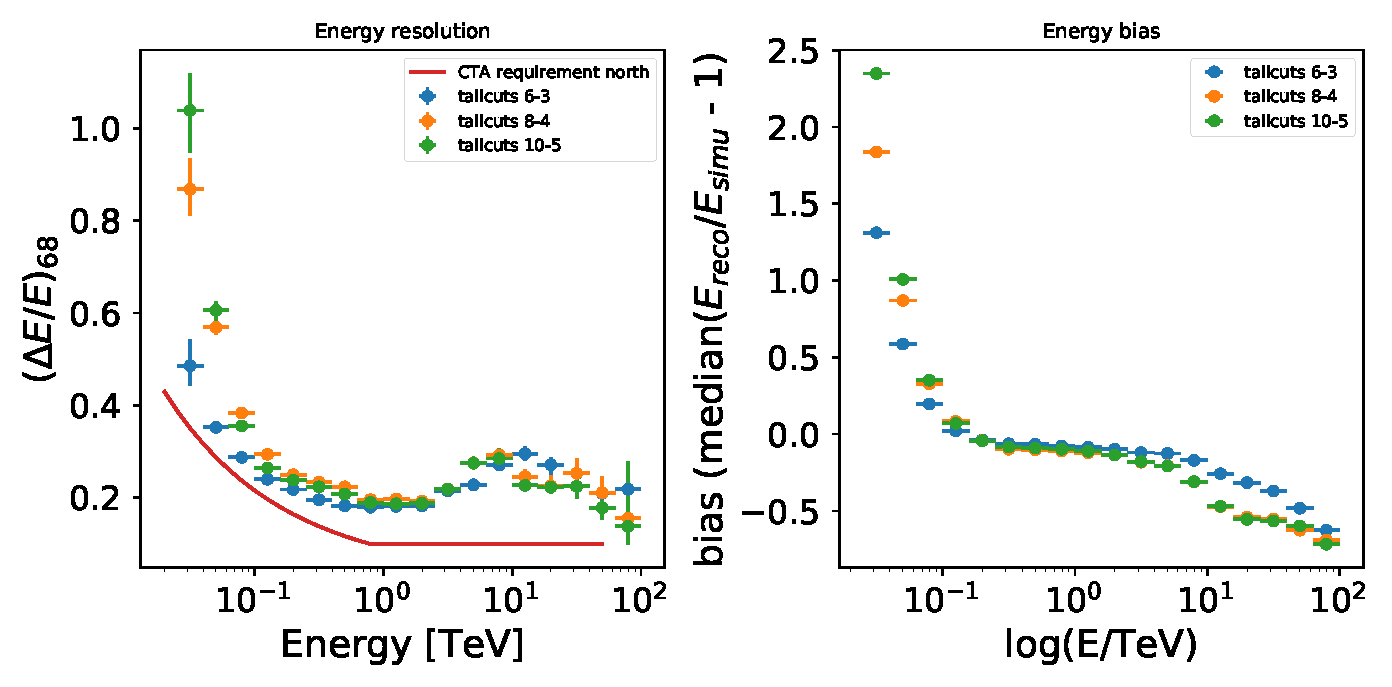
\includegraphics[width=1\textwidth]{Pictures/energy_resolution.pdf}
  \caption{Energy resolution for the \gls{lst}1 analysis applied to a \gls{mc} production of point-like $\gamma$ events, for three different sets of cleaning parameters (low level-high level threshold in number of photoelectrons). As a reference, the energy resolution requirement for \gls{cta}-north array is also shown. The energy resolution plot of the \textit{left} has been bias corrected.}
  \label{fig:energy}
\end{figure}

\subsubsection{Angular resolution}

The angular resolution is calculated similarly to the energy resolution, but in this case the relative error shown in figure \ref{fig:angres} refers to the angular difference between the true direction of the source and the reconstructed direction. As can be seen in the left plot from figure \ref{fig:angres}, the majority of gamma events concentrate in low $\theta^2$ angles, therefore, making cuts in this angle allows to discard background events. The features used for the disp vector regression ordered by their importance can be seen in figure \ref{fig:importances}.


\begin{figure}[h]
  \centering
  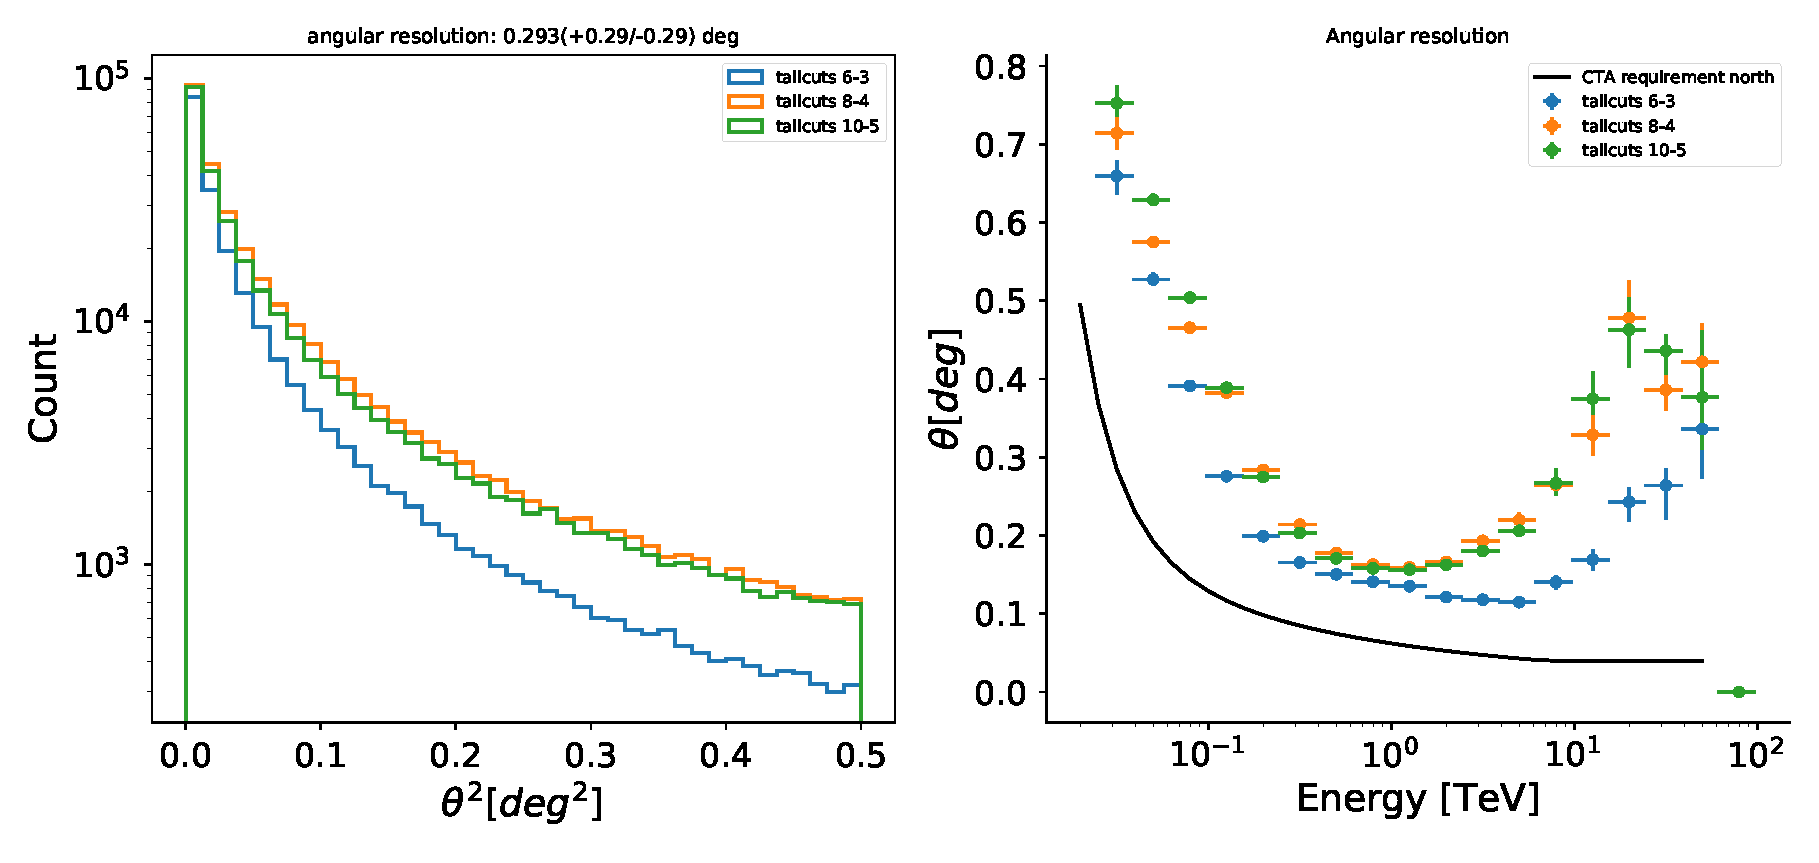
\includegraphics[width=1\textwidth]{Pictures/angular_resolution.pdf}
  \caption{\textit{Left:} $\theta^2$ plot for the \gls{mc} simulated $\gamma$ point-like events, using three sets of cleaning parameters. \textit{Right}: Angular resolution as a function of reconstructed energy.}
  \label{fig:angres}
\end{figure}

\subsubsection{$\gamma$-hadron separation}

The performance in $\gamma$-hadron separation can be studied in terms of the \gls{roc} curve of the \gls{rf} classifier. The \gls{roc} curve illustrates the diagnostic ability of a binary classifier as its discrimination threshold is varied. It is produced plotting the true positive rate (the rate of $\gamma$s correctly classified) versus the false positive rate (the rate of protons incorrectly classified as $\gamma$s) at several thresholds in gammaness. A value of 1 in true positive rate, while 0 in the false positive rate would mean a perfect classification. The closest of the \gls{roc} curve to a diagonal line, the more similar to a uniformly random distribution is the classification. For this result, shown in figure \ref{fig:roc}, a subset of protons was used to test the \gls{rf} classifier together with the point-like $\gamma$s. The features used for the $\gamma$/hadron classification ordered by their importance can be seen in figure \ref{fig:importances}.

\begin{figure}[h]
  \centering
  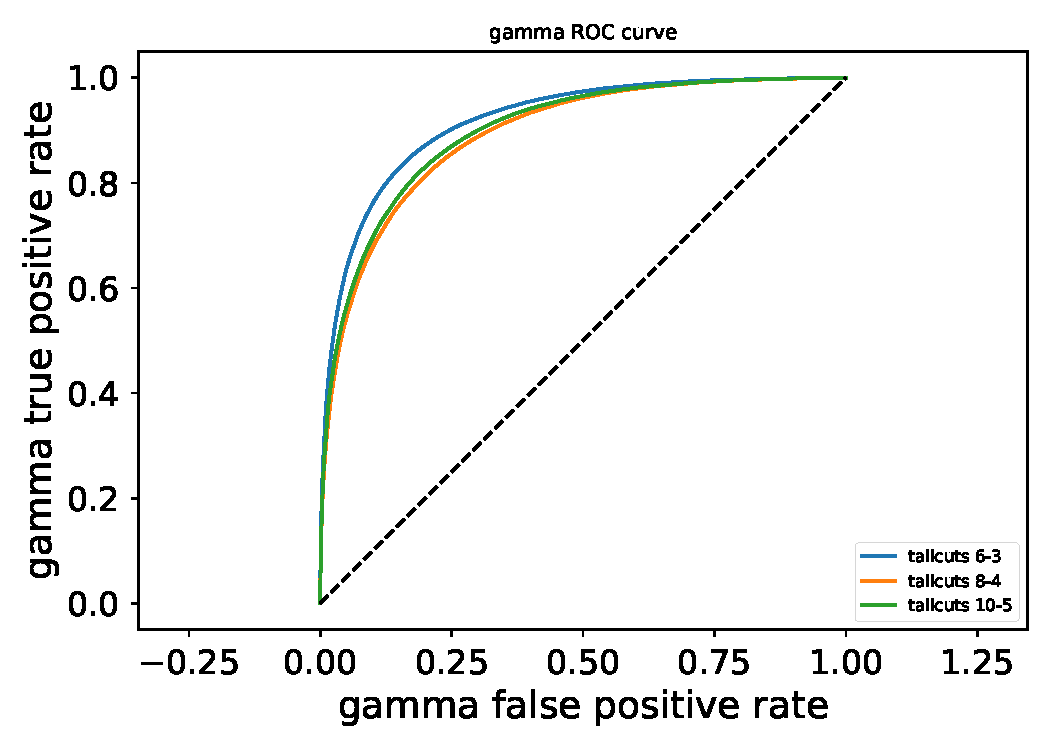
\includegraphics[width=0.6\textwidth]{Pictures/ROC.pdf}
  \caption{\gls{roc} curve of the \gls{rf} classifier applied to point-like gamma and diffuse proton events, for three different sets of cleaning parameters.}
  \label{fig:roc}
\end{figure}


\subsubsection{Sensitivity}

For the calculation of the sensitivity, a subset of proton events was used as background (off) events. Apart from the general cuts in intensity, width/length and leakage2 mentioned above, cuts in gammaness and $\theta^2$ were optimized to calculate the sensitivity. Subsets of point-like $\gamma$  and proton events were used to calculate the cuts in gammaness and $\theta^2$ which provided the best sensitivity in each of the 20 energy bins taken. The sensitivity was calculated for 10 cuts in gammaness and  10 in $\theta^2$ for each energy bin. The combination of cuts giving the lower sensitivity value, keeping a minimum of 10 $\gamma$ and proton events in the bin (both before and after re-weighting), was selected.
The resulting sensitivity was then calculated for a different subset of $\gamma$s and protons, applying the selected cuts. The sensitivity curve is shown in picture \ref{fig:sens}.

\begin{figure}[h]
  \centering
  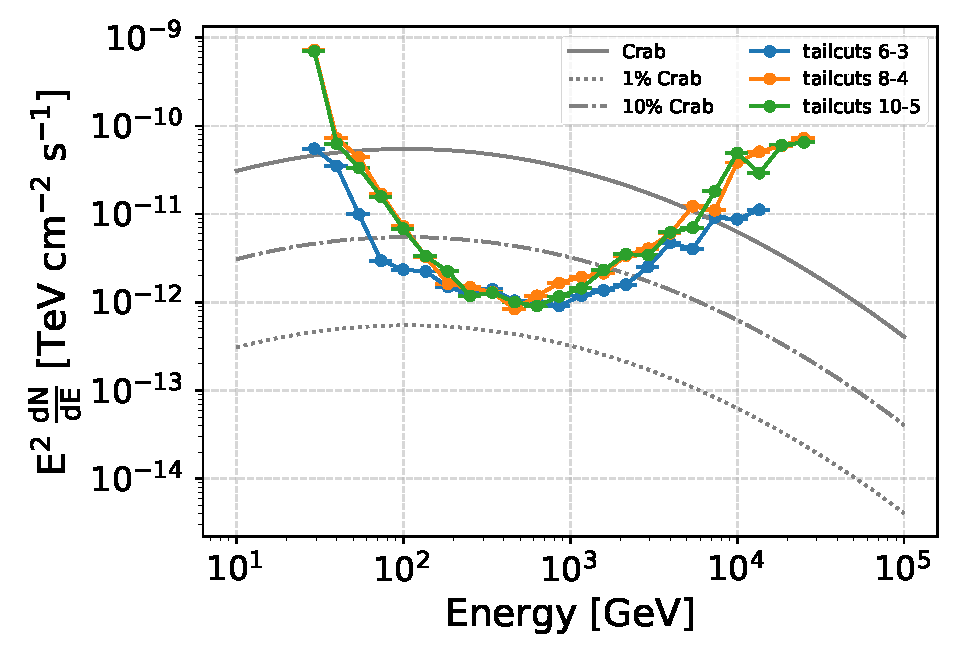
\includegraphics[width=0.8\textwidth]{Pictures/sensitivity.pdf}
  \caption{Sensitivity plot for 50h of observation of a point-like $\gamma$-ray source with a Crab-like spectrum, obtained by selecting the cuts in gammaness and $\theta^2$ which provided the best differential sensitivity per energy bin. As a reference, the spectra of Crab, 10\% of Crab and 1 \% of Crab flux are shown.}
  \label{fig:sens}
\end{figure}

\section[Expectation-Maximization method for Hillas Parameters...]{Expectation-Maximization method for Hillas Parameters calculation without cleaning} \label{sec:EM}

As explained in section \ref{sec:cleanpars}, cleaning methods often require the empirical adjustment of some parameters, to find a balance between a good enough background suppression without losing too much information from the shower. The cleaning parameters affect particularly the analysis of low energy showers. In the tailcuts method, too strong cleaning thresholds tend to eliminate many pixels of the already small low energy showers, making the task of $\gamma$-hadron separation much more difficult. Also, losing the ellipse shape of $\gamma$ showers lead to wrong calculation of Hillas parameters and consequently of the disp vector.\\
For all these reasons, to research for new analysis methods which could improve the performance of \gls{lst}, a method for image parameterization which does not require a previous cleaning has been developed in the scope of this thesis. It is based on the \gls{em} algorithm, where the light content in each pixel is recursively assigned to be part of the shower or the background. In the next sections, the basic concepts of the \gls{em} method and how it can be applied to images of showers will be summarized. Then some results comparing the \gls{em} with the classic cleaning method will be discussed.

\subsection{The Expectation-Maximization algorithm} \label{sec:em}

The \gls{em} algorithm \cite{1977EM} is an iterative method for calculating maximum likelihood estimates of model parameters, where the model depends on unobserved data or latent variables. These latent variables would be those that cannot be observed in the data set but still can influence other random variables. The algorithm will iterate until finding the model parameters and hidden variables that converge to a maximum likelihood estimation.\\
Given a statistical model which has generated a set of $X$ observed data points, which depends on a set of latent variables $Z$ and unknown parameters $\theta$, the basic iteration of the \gls{em} consist on two steps:

\begin{itemize}
\item \textbf{Expectation}: Creates an expectation function $Q(\theta | \theta^{(t)})$, which is the evaluation of the log-likelihood with the current estimate of the model parameters $\theta^{(t)}$, meaning it calculates the latent variables $Z$.
  \begin{equation}
    Q(\theta | \theta^{(t)}) = E_{Z|X,\theta^(t)}
  \end{equation}

\item \textbf{Maximization}: Maximizes the log-likelihood function found in the previous step to find a new set of estimated parameters.
  \begin{equation}
    \theta^{(t+1)} = arg max Q(\theta | \theta^{(t)})
  \end{equation}
\end{itemize}

A common problem that has been successfully solved by the \gls{em} algorithm is the mixture models problem, where there is a set of data produced by several density distribution functions, but it is impossible to know which distribution has produced each data point. This distinction between distributions would be the latent variable. This is the particular case we face with shower images. We have a distribution of light in the pixels of the camera, and we know that some photoelectrons come from Cherenkov light, and others belong to fluctuations in the \gls{nsb}. We want to know the fraction of light in each pixel which belongs to each of the distributions.
We assume that the Cherenkov light will follow a bi-dimensional Gaussian distribution which produces the typical elliptical shape in the image, and the background is simply a two-dimensional constant distribution. The parameters of the model will be the usual Gaussian parameters (mean and standard deviation in two dimensions) $\{x_{0}, y_{0},\sigma_{xx}, \sigma_{yy}, \sigma_{xy}\}$ and the latent variables will be the fraction of photoelectrons from the Cherenkov shower $n_{Ch}/n$ and from the background $n_{bkg}/n$ in each pixel with $n$ total photoelectrons.
The number of photoelectrons belonging to each distribution is:

\begin{equation}
  N_{i} = \sum_{pixels} P(pixel/i)\cdot N
\end{equation}

Where $N_i$ is the number of photoelectrons produced by the distribution $i$ (Cherenkov or background), $N$ is the total number of photoelectrons in the image and $P(pixel/i)$ is the probability of a photoelectron in the pixel to have been produced by the distribution $i$.\\
Using the Bayes theorem:
\begin{equation}\label{eq:bayes}
  P(pixel/i) = \frac{P_i(pixel) \cdot P_i}{P(pixel)}
\end{equation}
Where $P_i(pixel)$ is the probability of a photoelectron produced by the distribution $i$ to fall in the pixel, $P_i$ is the probability of a photoelectron to be produced by the distribution $i$ and $P(pixel)$ is the probability of a photoelectron to fall in the pixel. This last probability will actually be:
\begin{equation}
  P(pixel) = \sum_{i} P_i \cdot P_i(pixel)
\end{equation}
Where probabilities $P_i=(P_{Ch}, P_{Bkg})$ are equal to the fraction of photoelectrons in the image belonging to the shower(background) with respect to the total number of photoelectrons. The probabilities $P_i(pixel)$ can be written as:
\begin{equation}
  \begin{split}
    & P_{Ch}(pixel) = BiGaus(x_{0}, y_{0},\sigma_{xx}, \sigma_{yy}, \sigma_{xy}) \cdot A_{pixel}\\
    & P_{bkg}(pixel) = A_{pixel}/A_{total}
  \end{split}
\end{equation}
Where $A_{pixel}$ is the area of the pixel and $A_{total}$ the sum of the areas of all pixels.\\
The loop in the \gls{em} to solve this problem will go as follows:
\begin{enumerate}
\item An initial assumption of the Gaussian parameters is made. Because the bi-dimensional Gaussian corresponds to the Hillas ellipse, the means of the distribution will coincide with the center of gravity of the ellipse, which will be close to the pixel with the larger number of photoelectrons. To avoid choosing an outlier pixel, we take the initial means of the Gaussian ($x_0$, $y_0$) as the coordinates of the barycenter of the three more luminous pixels. The initial values of the standard deviations are set to arbitrary high values $\sigma_{xx}=20000$ mm, $\sigma_{yy}=20000$ mm, $\sigma_{xy}=0$ mm. Also we assume an initial estimation of the fraction of the light belonging to the shower and background as 50\% of the total number of photoelectrons for each.

\item \textit{Expectation}: Using the previous estimation of Gaussian parameters and fractions, equation \ref{eq:bayes} is solved and the new distributions of the shower and the background are obtained. For each pixel, the number of photoelectrons belonging to the shower and the background is calculated.

\item \textit{Maximization}: Using the distributions from previous steps, the parameters of the bi-dimensional Gaussian are calculated, and also the fraction of the total photoelectrons produced by each distribution (which is simply the sum of all shower and background pixels content respectively). The new Gaussian parameters will be:

  \begin{equation}
    \begin{split}
      & mean_{x} = \frac{1}{N}\sum_{pixels} n_{Ch} x_{pix}\\
      & mean_{y} = \frac{1}{N}\sum_{pixels} n_{Ch} y_{pix}\\
      & \sigma_{xx} = \frac{1}{N}\sum_{pixels} n_{Ch} x_{pix}^{2} - mean_{x}^2\\
      & \sigma_{yy} = \frac{1}{N}\sum_{pixels} n_{Ch} y_{pix}^{2} - mean_{y}^2\\
      & \sigma_{xy} = \frac{1}{N}\sum_{pixels} n_{Ch} x_{pix}^{2} y_{pix}^{2} - mean_{x}mean_{y}\\
    \end{split}
  \end{equation}
\item Steps 2 and 3 are repeated until convergence.\\

\end{enumerate}

Once the loop has ended, the parameters of the resulting Gaussian distribution are used to calculate the Hillas parameters as the first (x, y, r), second (width, length, $\phi$, $\psi$) and third order (skewness, kurtosis) moments of the distribution. The intensity (number of photoelectrons) of the shower, is simply the sum of the photoelectrons assigned to the Gaussian distribution by the algorithm.

\subsection{Comparison of \gls{em} without cleaning and tailcuts cleaning} \label{sec:compare_methods}

The \gls{em} method was used to calculate the Hillas parameters of the \gls{mc} production described in section \ref{sec:mcdata}. These parameters were used to train a new set of \glspl{rf} to perform the energy and direction reconstruction and the $\gamma$-hadron classification.
The results obtained with \gls{em} have been compared to those obtained applying a two-level tailcuts cleaning (6-3) before image parameterization as of the one used in section \ref{sec:performance}.
In this case, the \glspl{rf}, both for \gls{em} and tailcuts were trained without including the intercept parameter (see list of features in \ref{sec:rffeatures}). The reason is that by the time this section was written, this parameter was ruled out as a valid training feature in \textit{cta-lstchain} because there were reasons to believe it was strongly biasing the \glspl{rf} results. Therefore, the performance results shown in this section regarding the tailcuts method slightly differ from the ones of section \ref{sec:performance}.\\
In this section, results on energy resolution, angular resolution, and $\gamma$-hadron separation are shown comparing the two methods, with different cuts in intensity. Cuts in gammaness > 0.6 (except to produce ROC curves, where no cut in gammaness is applied),  leakage < 0.2, and width/length > 0.1 were also applied to the reconstructed events.

\begin{figure}[h!]
  \centering
  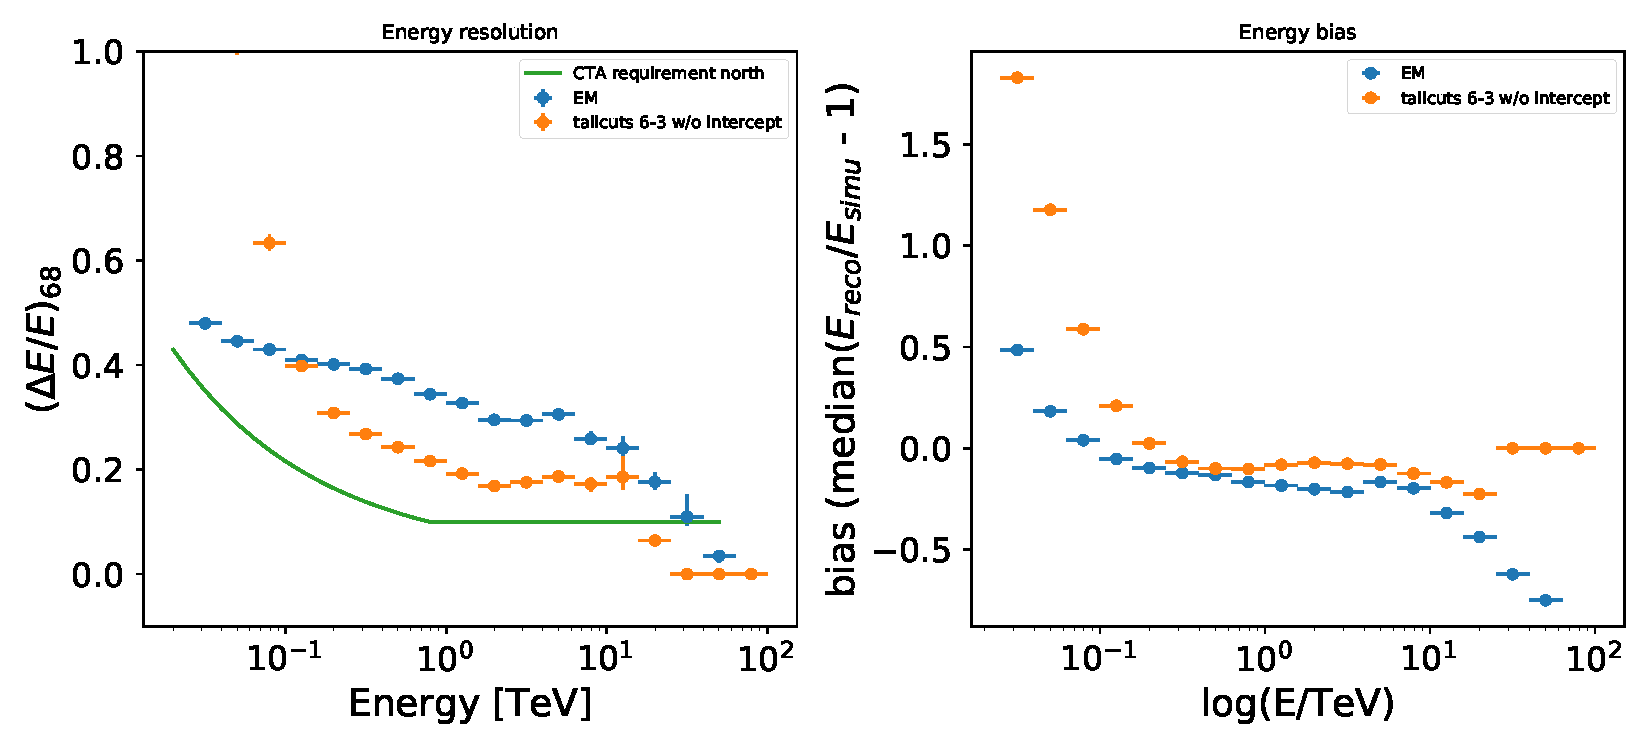
\includegraphics[width=0.8\textwidth]{{Pictures/em_energy_resolution_intensity100_gammaness0.6}.pdf}
  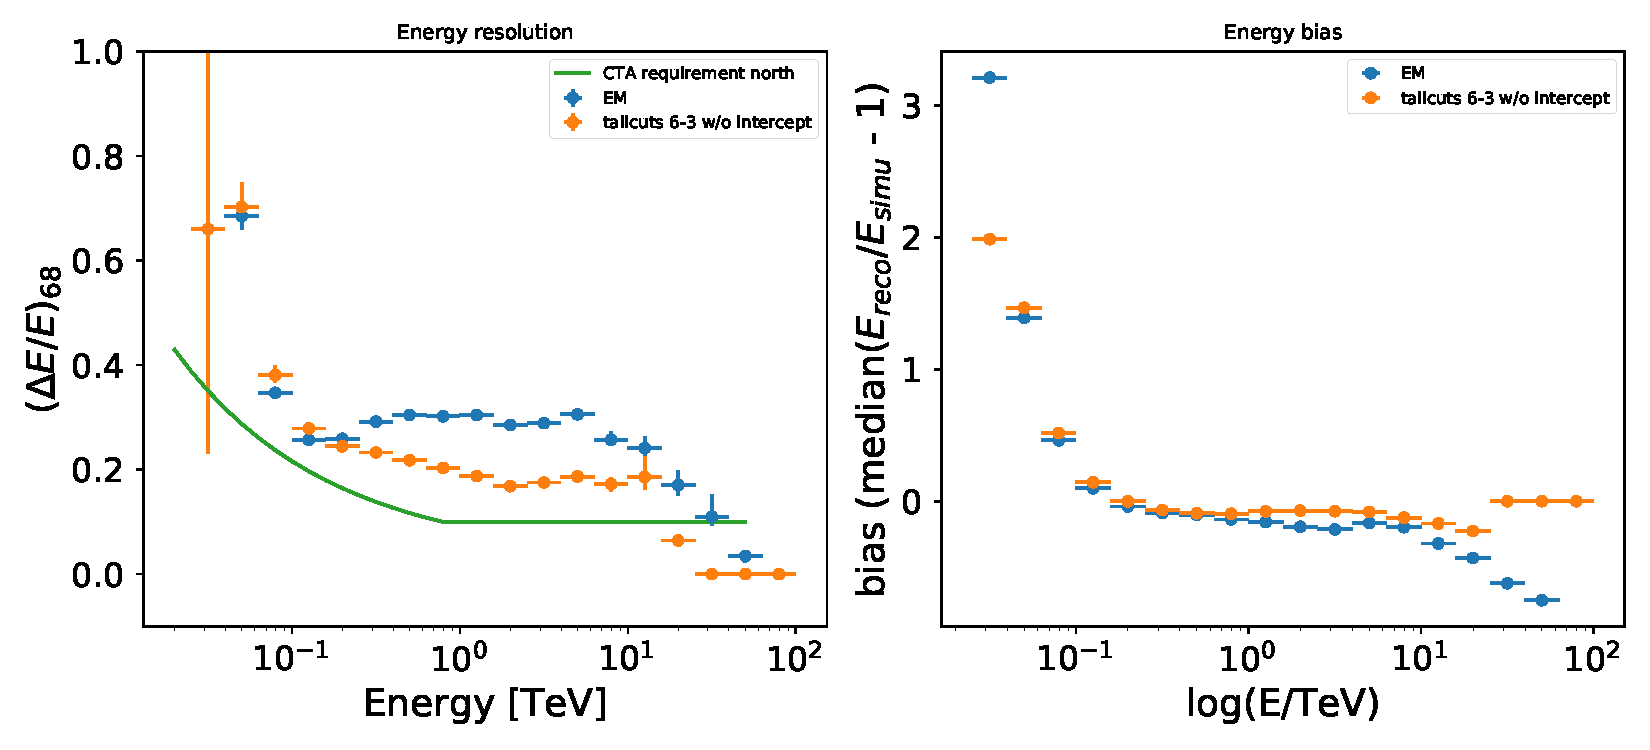
\includegraphics[width=0.8\textwidth]{{Pictures/em_energy_resolution_intensity500_gammaness0.6}.pdf}
  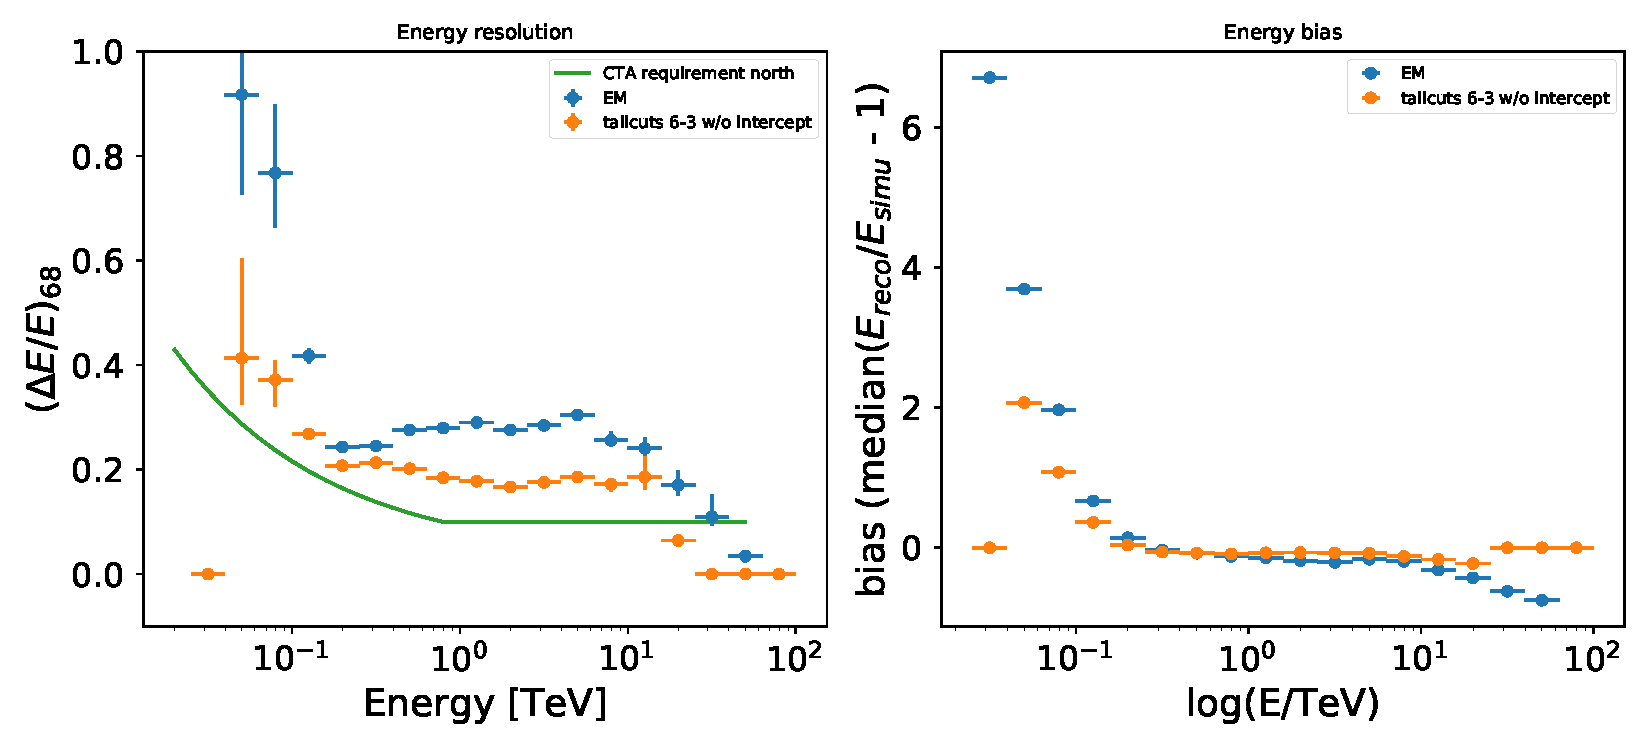
\includegraphics[width=0.8\textwidth]{{Pictures/em_energy_resolution_intensity1000_gammaness0.6}.pdf}
  \caption{Energy resolution plots for cuts in intensity > 100 phe(\textit{top}), > 500 phe (\textit{middle}) and > 1000 phe (\textit{bottom}) comparing the \gls{em} method for Hillas parameterization and the tailcuts cleaning method.}
  \label{fig:em_energy_res}
\end{figure}

\begin{figure}[h!]
  \centering
  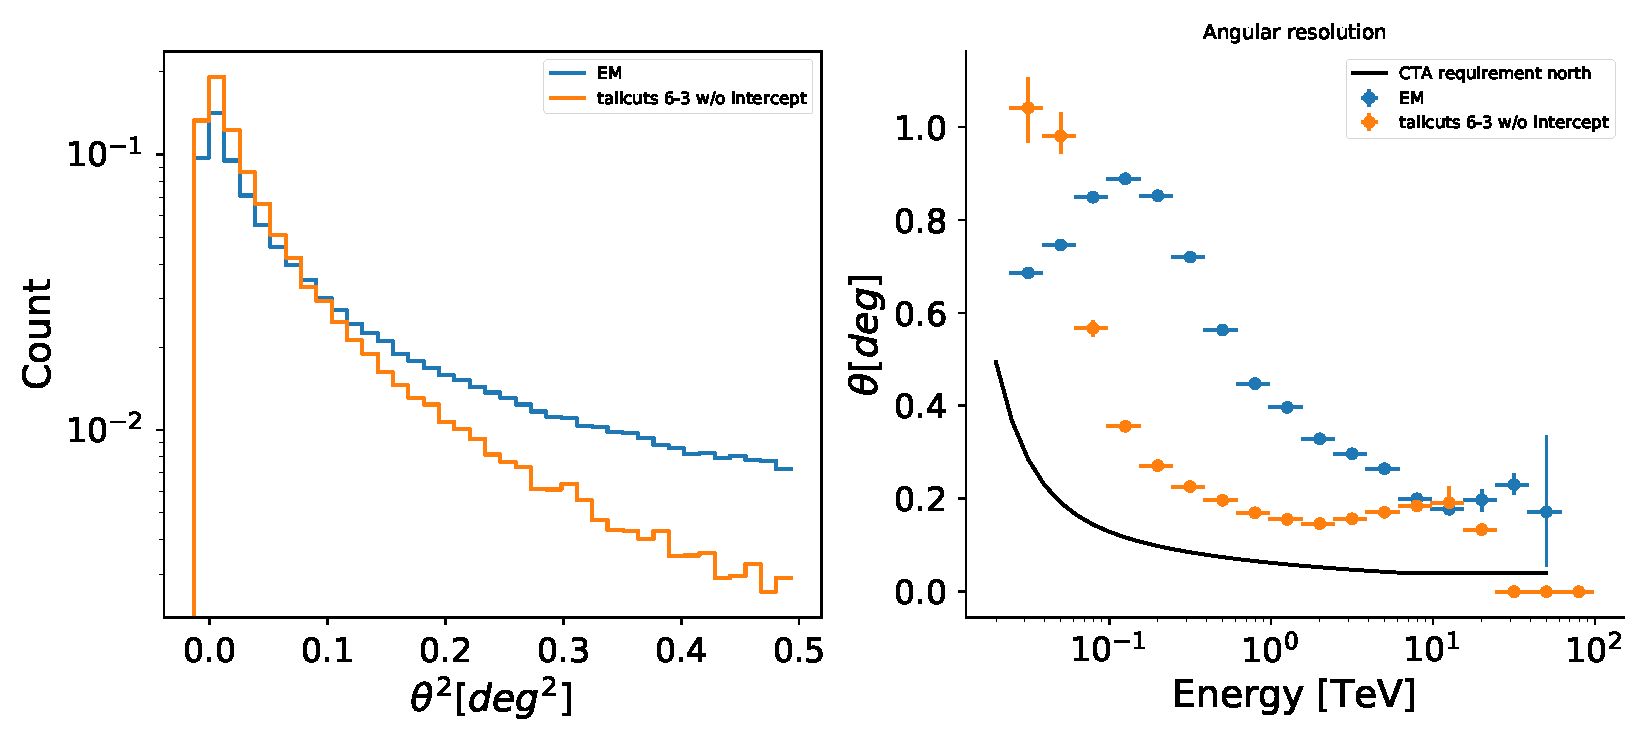
\includegraphics[width=0.8\textwidth]{{Pictures/em_angular_resolution_intensity100_gammaness0.6}.pdf}
  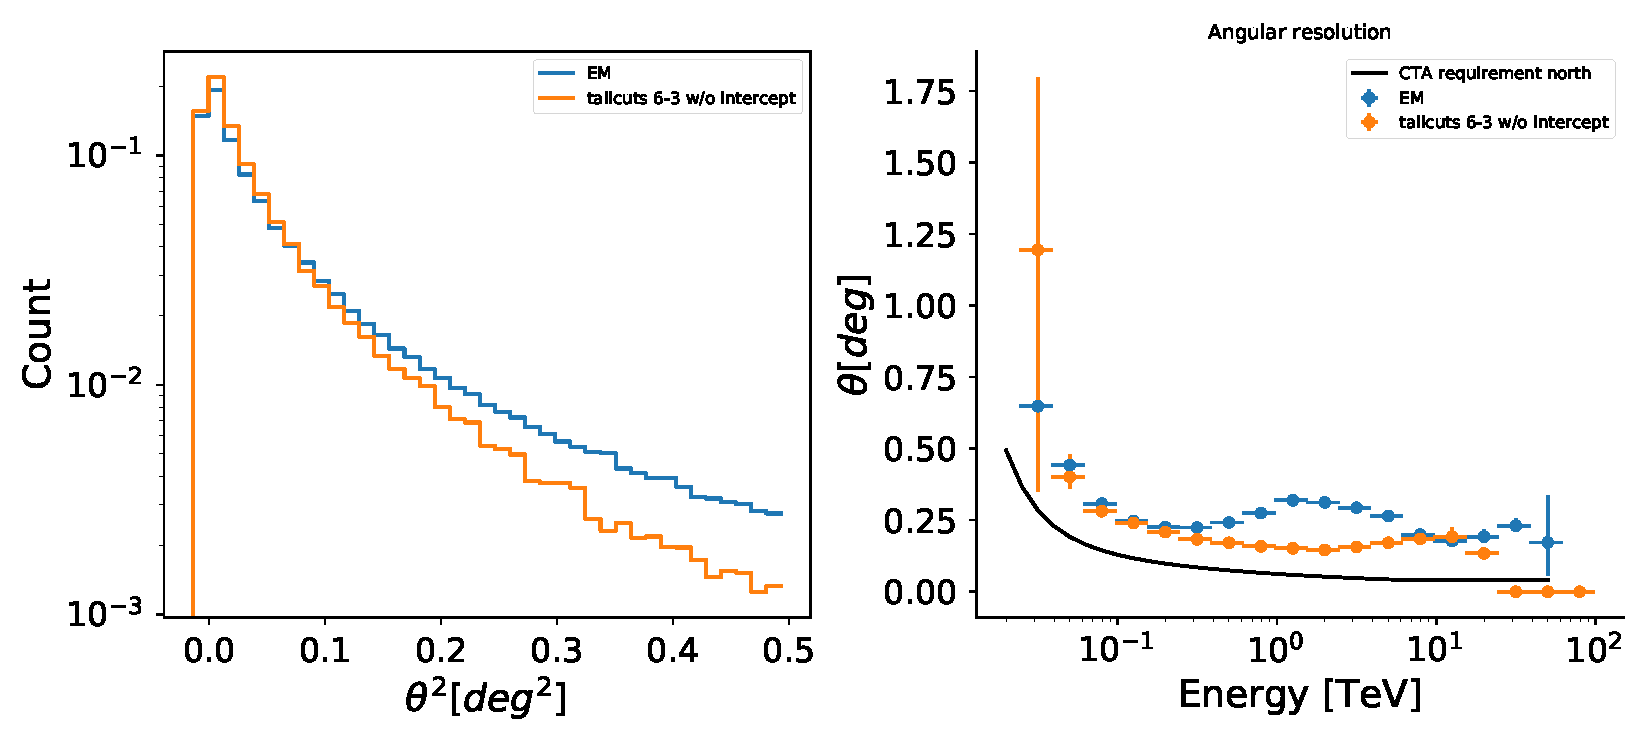
\includegraphics[width=0.8\textwidth]{{Pictures/em_angular_resolution_intensity500_gammaness0.6}.pdf}
  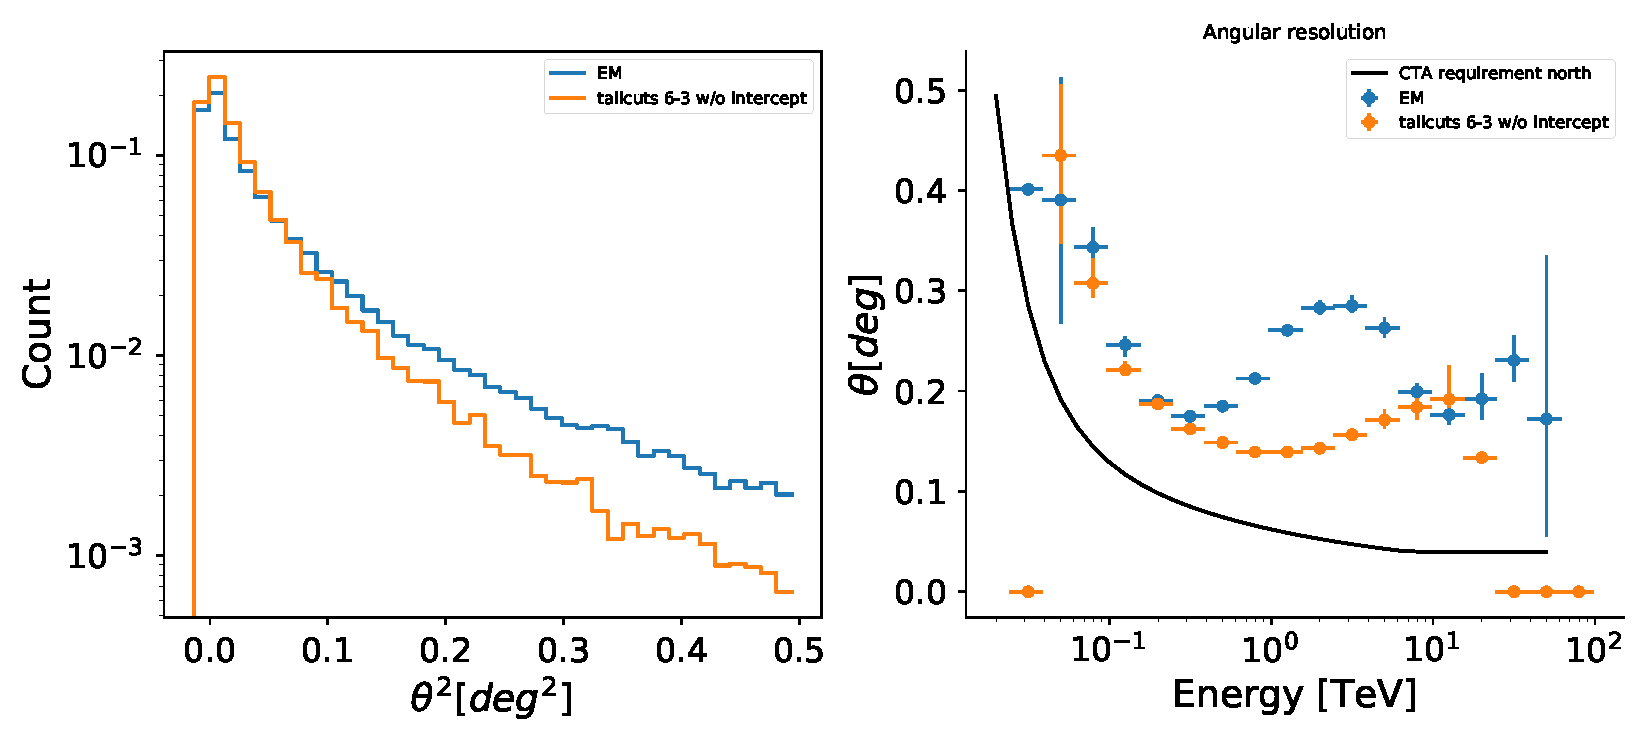
\includegraphics[width=0.8\textwidth]{{Pictures/em_angular_resolution_intensity1000_gammaness0.6}.pdf}
  \caption{Angular resolution plots for cuts in intensity > 100 phe(\textit{top}), > 500 phe (\textit{middle}) and > 1000 phe (\textit{bottom}) comparing the \gls{em} method for Hillas parameterization and the tailcuts cleaning method.}
  \label{fig:em_angular_res}
\end{figure}

\begin{figure}[h!]
  \centering
  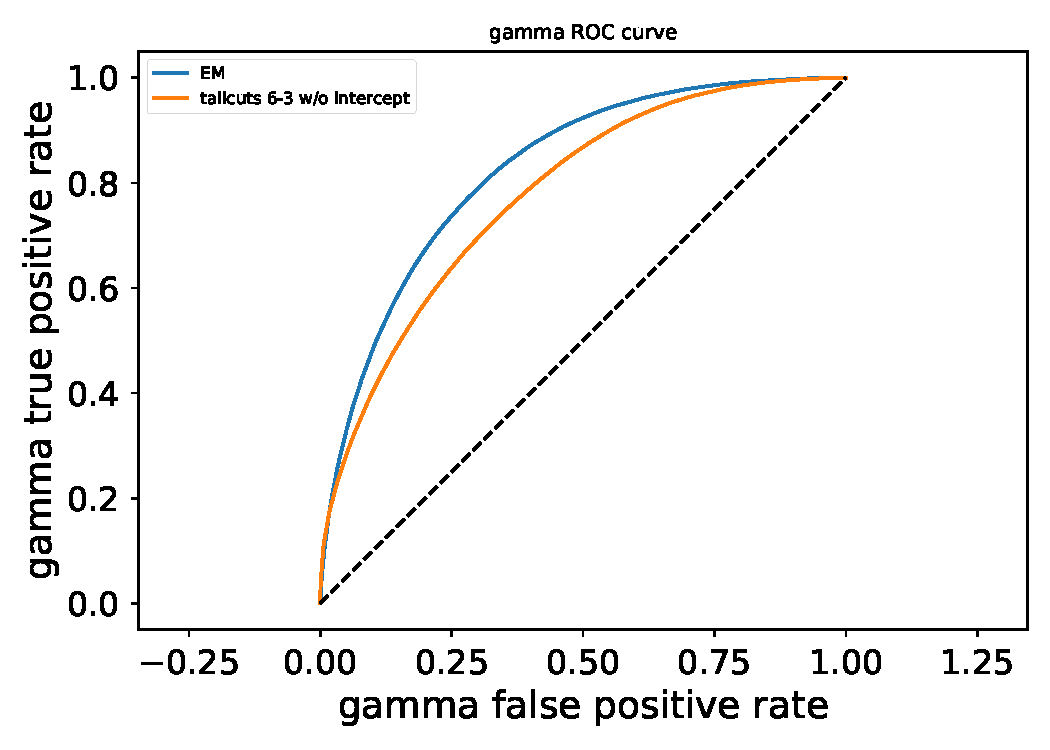
\includegraphics[width=0.5\textwidth]{Pictures/em_ROC_intensity100.pdf}\\
  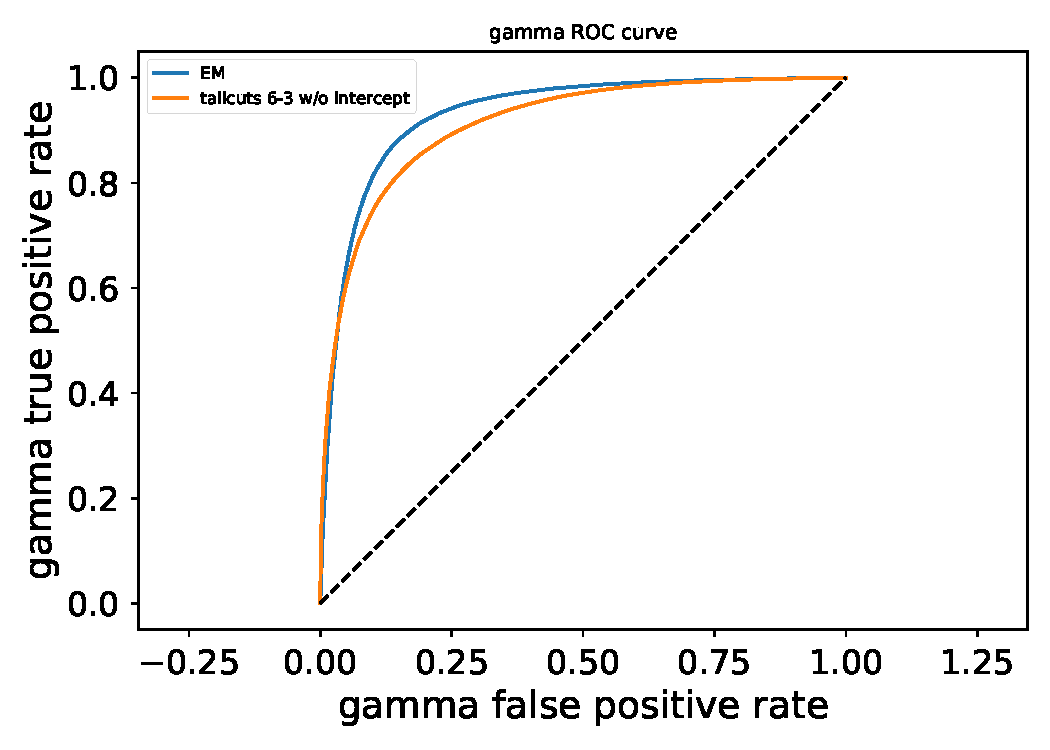
\includegraphics[width=0.5\textwidth]{Pictures/em_ROC_intensity500.pdf}\\
  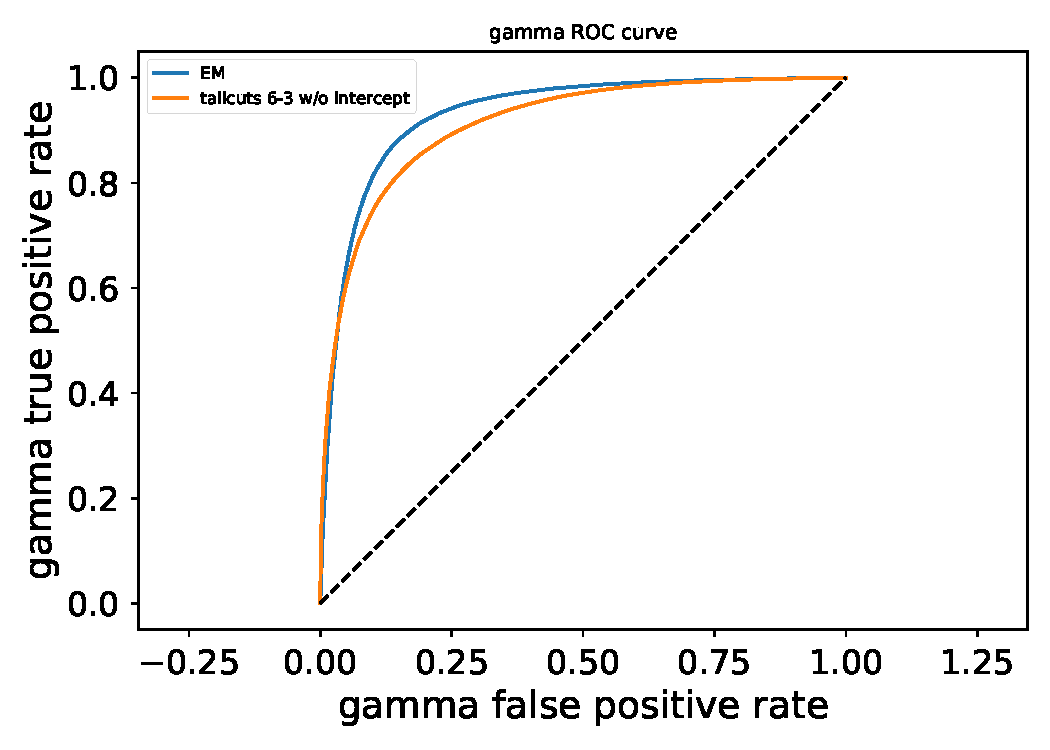
\includegraphics[width=0.5\textwidth]{Pictures/em_ROC_intensity1000.pdf}
  \caption{ROC curves for cuts in intensity > 100 phe(\textit{top}), > 500 phe (\textit{middle}) and > 1000 phe (\textit{bottom}) comparing the \gls{em} method for Hillas parameterization and the tailcuts cleaning method.}
  \label{fig:em_ROC}
\end{figure}

From figures \ref{fig:em_energy_res} and \ref{fig:em_angular_res}, it appears that the performance of the \gls{em} method is worse than the tailcuts for the majority of the energy range, except for the lower energy bins when a small cut in intensity (> 100) is applied. This supports the hypothesis that the tailcuts cleaning tends to lose information from showers with a low number of photoelectrons, while \gls{em} preserves the information of the full image. Despite these results, it is interesting to observe how according to the \gls{roc} curves in figure \ref{fig:em_ROC}, the \gls{em} seems to perform a better classification than the tailcuts cleaning. Further discussion on this issue, which shows interesting results when applying the method to real data, is given in section \ref{sec:em-real}.

\section{Results on real data} \label{sec:realdata}

Since the beginning of the commissioning of the telescope, three Crab data taking campaigns have been carried on, where the Crab nebula has been observed with the \gls{lst}1 during several nights, to test the performance of the whole instrument and the analysis tools.\\
In this section the data taken during the three Crab campaigns have been analyzed following the methods described in previous sections, deriving the final detection significance of the Crab over the total observation time of each campaign, after applying different cuts in intensity and gammaness. Telescope data is taken in several runs of a certain duration, where events are recorded and stored in fits files. Each night, four kinds of runs are taken: DRS4 calibration runs (for pedestal subtraction), camera calibration runs (see section \ref{sec:calib}) and data runs of two types: on and off runs. Data on runs are taken pointing with the telescope to the $\gamma$-ray source, in this case the Crab nebula. Off runs are taken pointing to a region without a $\gamma$-ray sources, where the \gls{cr} background is similar to that of the on region, to extract the signal events as an excess over the background in the on.\\
The data runs have been calibrated and parameterized using \textit{cta-lstchain} following the steps described in section \ref{sec:anachain}. The signal extractor used has been the \textit{GlobalPeakWindowSum}  and the cleaning method applied is a two-level tailcuts with $Th_{high}=6$ phe and $T_{low}=3$ phe. The \gls{rf} models for energy and direction reconstruction, and $\gamma$/hadron separation have been trained with \gls{mc} data, as described in sections \ref{sec:recoe} and \ref{sec:gammahsep}, and applied to the on and off data for reconstruction to DL2 data level. The intercept parameter was not included among the \gls{rf} features. Quality cuts in leakage < 0.2 and width/length > 0.1 were applied, while cuts in intensity and gammaness have been optimized to obtain the best results.\\
In the on region, close to the source position, an excess of events should be observed compared to the background. At further distances, the rate of events should be comparable to that of the off region, where there are only background events. The number of background events $N_{bkg}$ in the on region can be estimated as $N_{off}$ multiplied by a normalization factor \footnote{This factor $n$ is equivalent to the factor $\alpha$ of section \ref{sec:sensitivity}. In the present section the name has been changed to not be confused with the $\alpha$ angle, described below.}, $n = N_{on}/N_{off}$ calculated at a large distance from the assumed source position (the center of the camera), which accounts for the difference in observation time of the two regions. The significance of the excess in the on region is calculated using the Li\&Ma formula \cite{1983LiMa}, \cite{2005LiMa} (see also section \ref{sec:sensitivity}):

\begin{equation}
  S = \sqrt{2} \left(N_{on}\cdot ln\left( \frac{(1+n)N_{on}}{n(N_{on}+N_{off})}\right)+N_{off}\cdot ln\left( \frac{(1+n)N_{off}}{N_{on}+N_{off}}\right) \right)^{1/2}
\end{equation}

The normalization factor $n$ has been calculated using the $\alpha$ angle, which is defined as:

\begin{equation}
  \alpha = arc cos\left(\frac{X_{c.o.g.}cos(\psi) + Y_{c.o.g.} sin(\psi)}{X_{c.o.g.}^2 + Y_{c.o.g.}^2}\right)
\end{equation}

Where $X_{c.o.g.}$ and $Y_{c.o.g.}$ are the coordinates of the center of gravity of the Hillas ellipse of the shower image, and angle $\psi$ is the angle between the semi-major axis of the ellipse and the line between the center of the camera and the centroid of the ellipse. The $\alpha$ angle is a measure of how deviated is the Hillas ellipse from pointing towards the center of the camera. Events with a high $\alpha$ angle are more likely to be background events, whereas $\gamma$ events will point towards the same position, close to the center, having small $\alpha$ angles. To estimate the background normalization factor $n$, events with $\alpha$ angle between 20º and 70º have been used. To calculate the excess signal and sensitivity, a cut in $\alpha < 8º$ is applied.\\
The rate of $\gamma$ events (number of events per minute) can be calculated dividing the number of excess events $N_{ex}=N_{on}-n N_{off}$ by the total observation time.\\
The $\alpha$ plots of the three campaigns are shown in pictures \ref{fig:1st-crab-campaign}, \ref{fig:2nd-crab-campaign} and \ref{fig:3rd-crab-campaign}, for different cuts in intensity and gammaness, to show the effect of these cuts in the significance. For the first Crab campaign, the best cuts of intensity > 1000 and gammaness > 0.6 resulted in a significance of $24.38 \sigma$ in 4.5 h of total observation time. For the second Crab campaign the best cuts were intensity > 500 and gammaness > 0.6, giving a total significance of $22.31\sigma$ for 7.8h of observation. The same cuts for the third Crab campaign resulted in a significance of $15.48\sigma$ for 6.1 h of observation.\\
During the commissioning of the telescope, several tests are performed in all the subsystems, along with updates and changes in the configuration. These activities affect the performance, making it very variable throughout the different observation nights. For that reason, it is necessary to keep track of how the performance varies from one campaign to the next. In picture \ref{fig:sig_evolution} the evolution of the significance with the square root of observation time along the three campaigns can be observed. This result will be compared with the future data taking campaigns, to characterize the stability of the telescope in the commissioning phase.

\begin{figure}[h!]
  \centering
  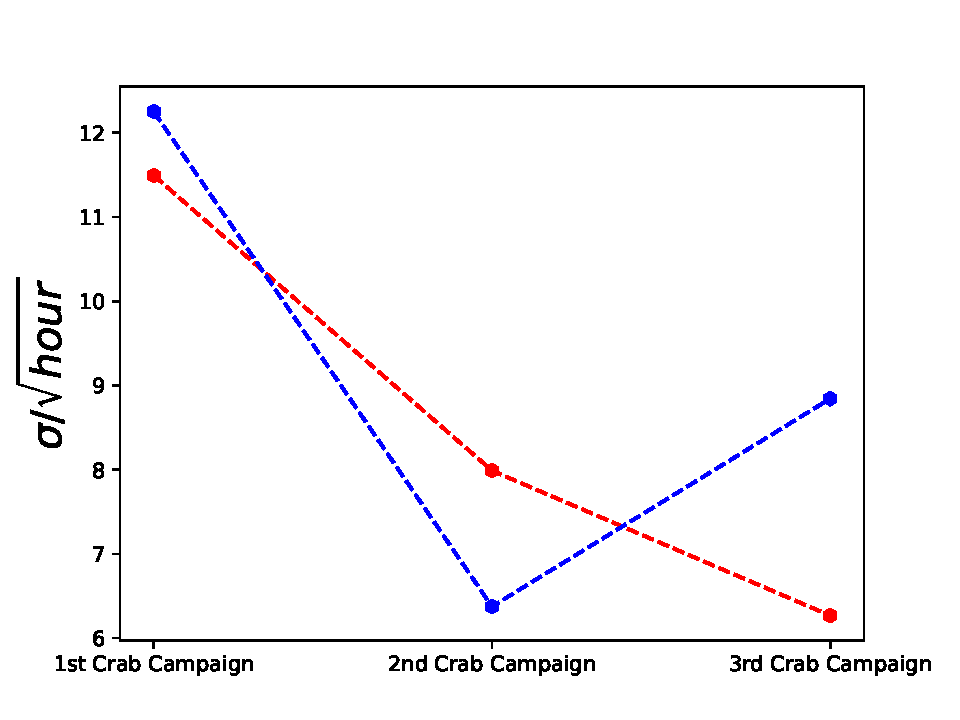
\includegraphics[width=0.7\textwidth]{Pictures/total_S.pdf}
  \caption{Evolution of the maximum significance per square root of time during the three Crab Campaigns. The red line shows the evolution when parameterizing the data applying a tailcuts cleaning, while the red line shows the significance obtained when using the \gls{em} method. Note that for each campaign, the maximum significance has been obtained applying different cuts in intensity and gammaness, as described in sections \ref{sec:realdata} and \ref{sec:em-real}.}
  \label{fig:sig_evolution}
\end{figure}

\subsection{Analysis of Crab Campaigns with Expectation-Maximization method for Hillas Parameterization} \label{sec:em-real}

The data from the full three Crab campaigns was reduced from R0 to DL2 data level using the \gls{em} method to calculate the Hillas parameters, without applying a tailcuts cleaning to the shower images. To reconstruct the energy and direction of the primaries, and to perform the $\gamma$-hadron separation the \glspl{rf} trained for section \ref{sec:compare_methods} were used. The alpha plots, computed using the same approach as described in section \ref{sec:realdata}, for the three campaigns are shown in pictures \ref{fig:em_1st-crab-campaign}, \ref{fig:em_2nd-crab-campaign} and \ref{fig:em_3rd-crab-campaign}, for different cuts in gammaness and intensity.\\
Note that for the \gls{em} parameterized data, the higher significance is reached with a lower cut in intensity than for the tailcuts cleaning based analysis (intensity > 100). As can be seen in picture \ref{fig:intensitydistribution}, the majority of showers have an intensity value between 100 and 1000 photoelectrons. A cut in intensity > 500, or 1000 photoelectrons, which is required to obtain the maximum sensitivity when applying the tailcuts cleaning (see pictures \ref{fig:1st-crab-campaign}, \ref{fig:2nd-crab-campaign} and \ref{fig:3rd-crab-campaign}), suppose to discard a huge number of recorded events. Because intensity and energy are directly related, those discarded events correspond to the lower energies.

\begin{figure}[h!]
  \centering
  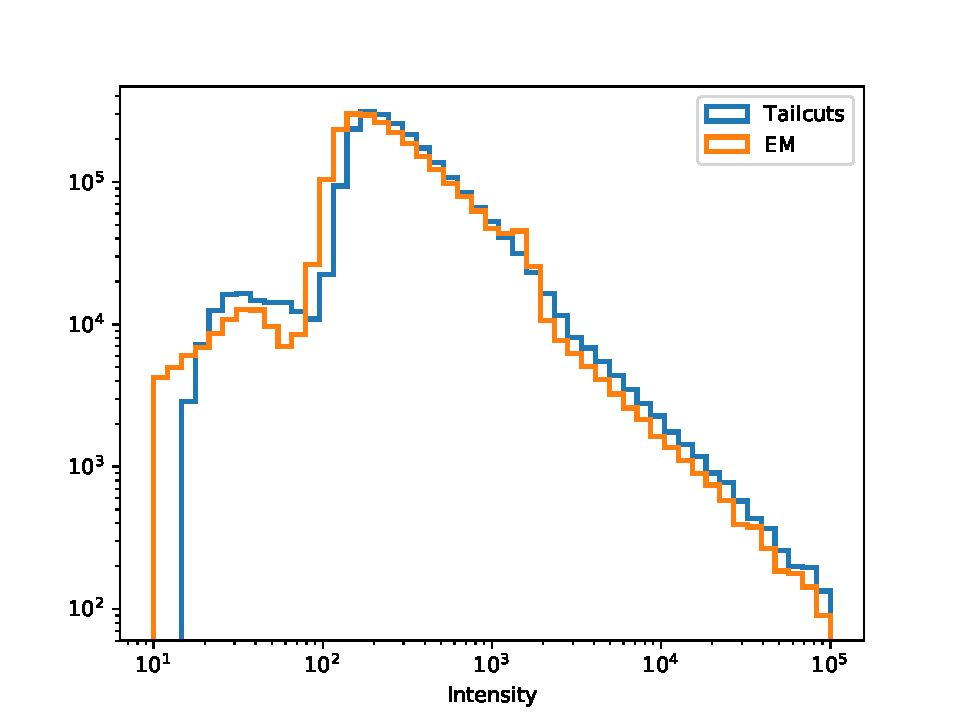
\includegraphics[width=0.7\linewidth]{Pictures/compare_intensity_distribution.pdf}
  \caption{Distribution of intensity of the showers for a subset of real data events, reduced using the \gls{em} method (\textit{orange}), and applying the tailcuts cleaning (\textit{blue}).}
  \label{fig:intensitydistribution}
\end{figure}

To understand this difference in the optimum intensity cuts, it is necessary to study how the parameterization performed with both methods is affecting the $\gamma$-hadron classification of the showers. The gammaness distributions of a set of \gls{mc} $\gamma$ and proton events, which were produced applying the tailcuts cleaning and the \gls{em} method are shown in figure \ref{fig:gammanessdist}, for two cuts in intensity (100 and 500 photoelectrons). The \gls{em} tends, in general, to give higher values of gammaness to $\gamma$ events, even for low intensities, while when applying the tailcuts cleaning, the majority of events are classified with low values of gammaness. In figure \ref{fig:em_ROC}, the ROC curves showed that the classification of the \gls{em} is better for any cut in intensity. The \gls{em} recovers a big number of $\gamma$ events which would be classified as protons when applying the tailcuts cleaning. In figure \ref{fig:fractiongammaness}, the fraction of the total of $\gamma$ and proton events that are left after different cuts in gammaness are shown for the \gls{em} and tailcuts method. For a cut in intensity >100 and gammaness of 0.7 (which are the optimum cuts in real data for the \gls{em} method), close to a 40\% more of true $\gamma$ events would be correctly classified as $\gamma$s with the \gls{em}. On the other hand, because the \gls{em} tends to assign higher values of gammaness also to proton events, the number of protons that survive the cut contributing to the background raises in a 10\%. This explains the higher number of events, and higher rates in the $\alpha$ plots computed with the \gls{em}, in comparison with the tailcuts cleaning method.\\
The \gls{em} recovers a large number of $\gamma$ events that do not survive the gammaness cut when using the tailcuts method, but on the other hand, keeps a larger background of hadron events. These two effects seem to compensate in the end, resulting in a similar final significance, but lowering the intensity cut and therefore, preserving more low energy events.
Keep low energy events still having a good background rejection is fundamental to lower the energy threshold of \gls{lst}1 in single telescope mode. The \gls{em} method has proven to be a potential tool to accomplish this task and its refinement and a better understanding of its effect in the reconstruction can suppose an improvement in the performance of the telescope during its commissioning phase.


\begin{figure}
  \centering
  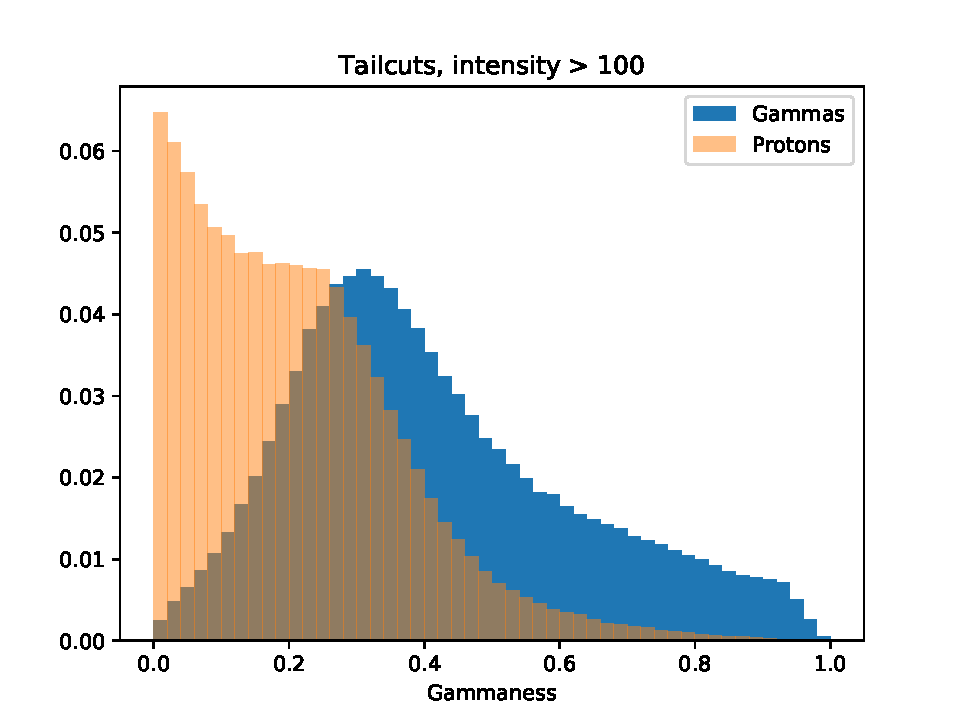
\includegraphics[width=0.45\textwidth]{Pictures/mc_gammaness_intensity100_likelihood10000000.pdf}
  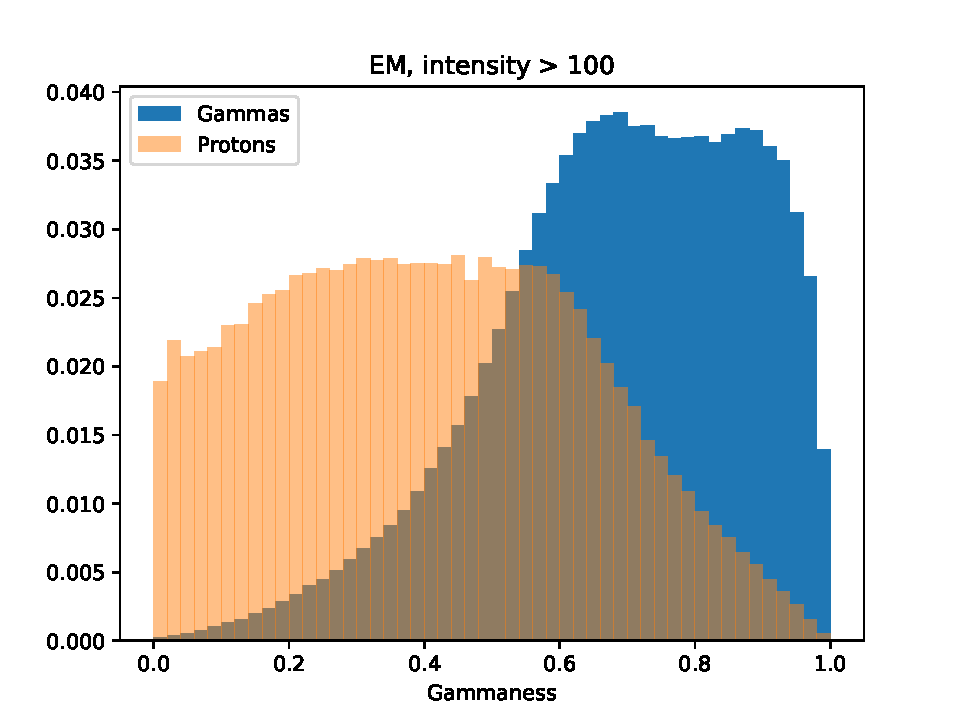
\includegraphics[width=0.45\textwidth]{Pictures/em_mc_tailcuts_gammaness_intensity100.pdf}\\
  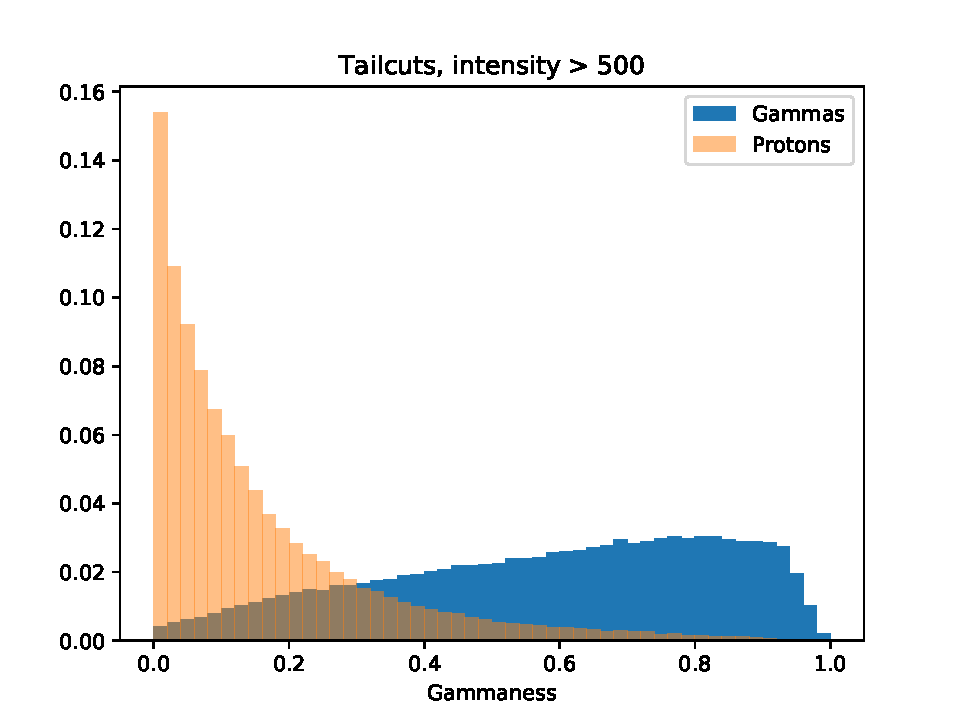
\includegraphics[width=0.45\textwidth]{Pictures/mc_gammaness_intensity500_likelihood10000000.pdf}
  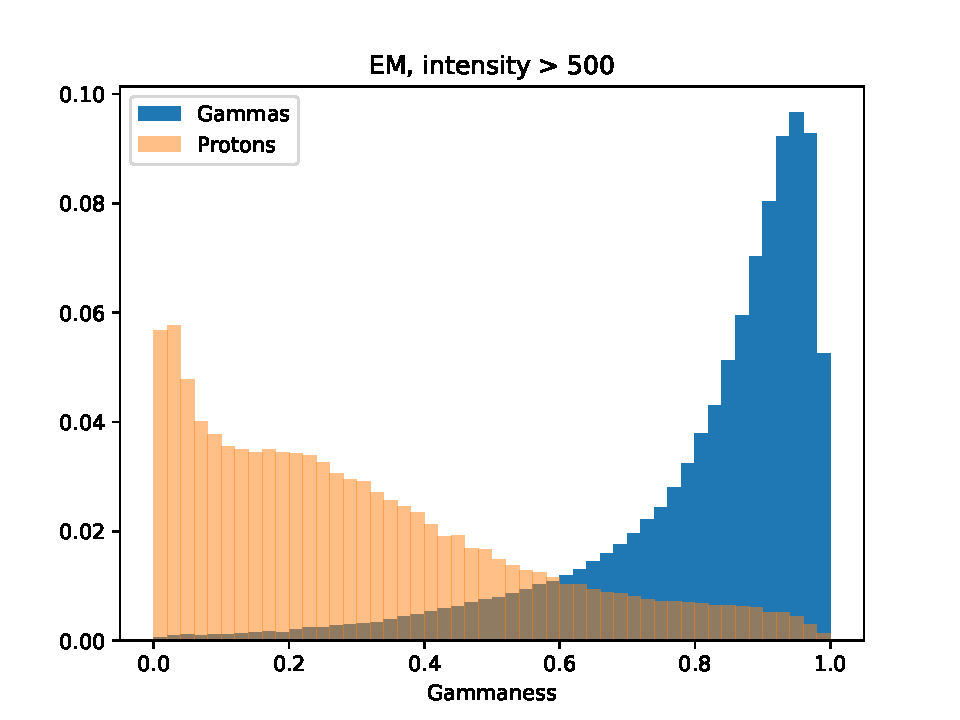
\includegraphics[width=0.45\textwidth]{Pictures/em_mc_tailcuts_gammaness_intensity500.pdf}
  \caption{Gammaness distribution (normalized) of a subset of \gls{mc} $gamma$ and proton events, parameterized after applying a tailcuts method (\textit{left}) and with the \gls{em} method without cleaning (\textit{right}, with cuts in intensity > 100 (\textit{top}) and 500 (\textit{bottom} photoelectrons.}
  \label{fig:gammanessdist}
\end{figure}


\begin{figure}[h!]
  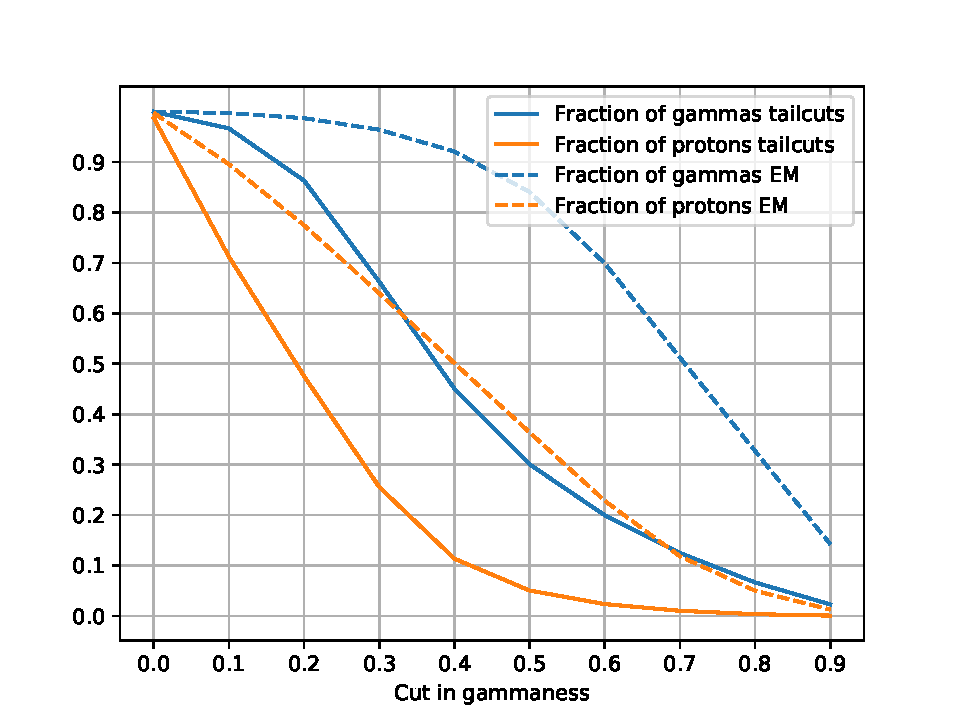
\includegraphics[width=0.45\linewidth]{Pictures/fraction_of_protons_gammas_intensity100-1000000.pdf}
  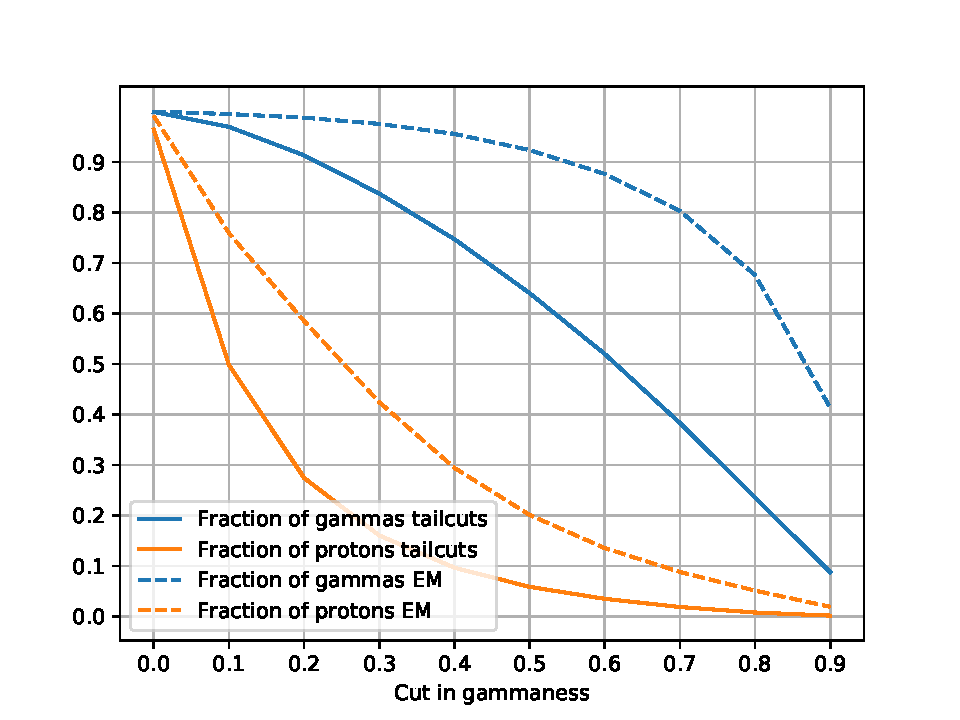
\includegraphics[width=0.45\linewidth]{Pictures/fraction_of_protons_gammas_intensity500-1000000.pdf}
  \caption{Fraction of $\gamma$ and proton events that would be left after making different cuts in gammaness (x axis) for a cut in intensity > 100 phe (\textit{left}) and > 500 phe (\textit{right}). That is the fraction that would be calssified as $\gamma$ events. Continuous line refers to the events reduced with the tailcuts cleaning, while dashed line represent events reduced using the \gls{em} method for Hillas parameterization.}
  \label{fig:fractiongammaness}
\end{figure}



\section{Summary and conclusion}

In this chapter, the chain for the single telescope data analysis of \gls{lst}1 has been described, and successfully applied to \gls{mc} simulated events, to compute the performance of the \gls{lst}1. Also, it has been used to analyze the first real data taken with the instrument, obtaining the detection significance of the Crab Nebula for the three data taking campaigns carried on up to the date this thesis is being written.\\
About the performance estimated using \gls{mc} simulations, it has been shown that the energy resolution reaches an error as low as 20\% in the range from $\sim 100$ GeV to a few TeV and the angular resolution in the same energy range is $\sim 0.2$º. From the three sets for tailcuts parameters, the one giving the best results has been the 6-3 tailcuts. The best sensitivity of \gls{lst}1 for 50 hours of observation is reached in the range between 100 GeV and 1 TeV, going below the 10\% of the Crab flux.\\
Regarding real data, the analysis chain designed for \gls{lst}1 has been successfully applied to the three Crab campaigns where Crab nebula data has been taken using the \gls{lst}1 between November 2019 and February 2020. The code has allowed to reconstruct the recorded events and to calculate the significance of detection of the source in terms of the $\alpha$ angle.\\
The \gls{em} method has been presented as a potential alternative for Hillas parameterization without applying a cleaning to the shower images, which avoids the necessity of adjusting the cleaning parameters. While the performance in energy and angular resolution was not as good as with the tailcuts cleaning method when compared in the same conditions, it offered an interesting result for the $\gamma$-hadron classification, especially improving the classification of low energy/low intensity showers.
This method has also been applied to the data of the three Crab campaigns, finding a similar significance as for the tailcuts method, but allowing to keep lower intensity showers. This result implies that the \gls{em} would be more efficient in classifying low energy showers, being a potential tool to lower the energy threshold of the telescope. Further investigation of this issue, retrieving the spectral information of the recorded data would be the next step to validate the method to improve the telescope performance in a wider energy range.

\begin{figure}[h]
  \begin{subfigure}{0.32\textwidth}
    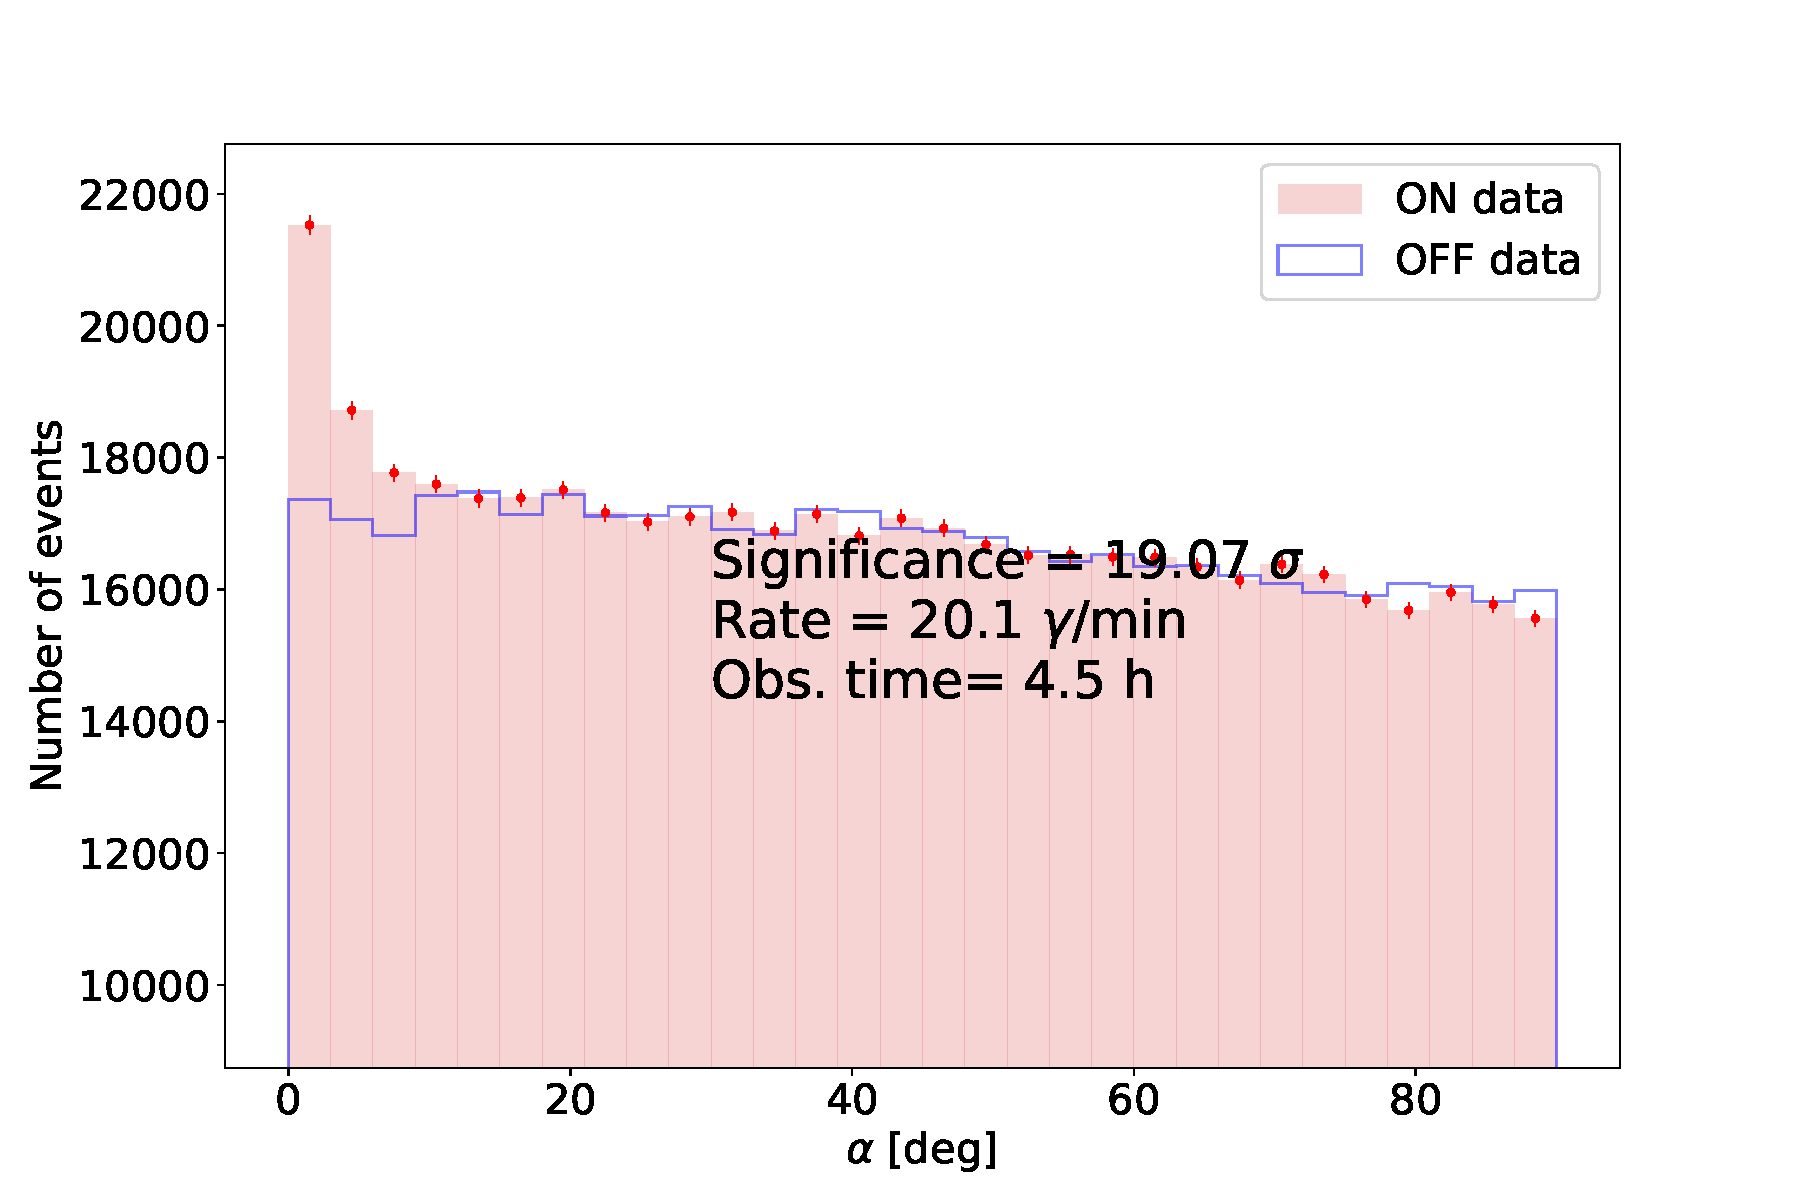
\includegraphics[width=\linewidth]{{Pictures/alphaplot_1stCrabCampaign_int100_gammaness0.50}.pdf}
    \caption{\small Intensity > 100, gammaness > 0.5} \label{fig:1st-a}
  \end{subfigure}
  \hspace*{\fill} % separation between the subfigures
  \begin{subfigure}{0.32\textwidth}
    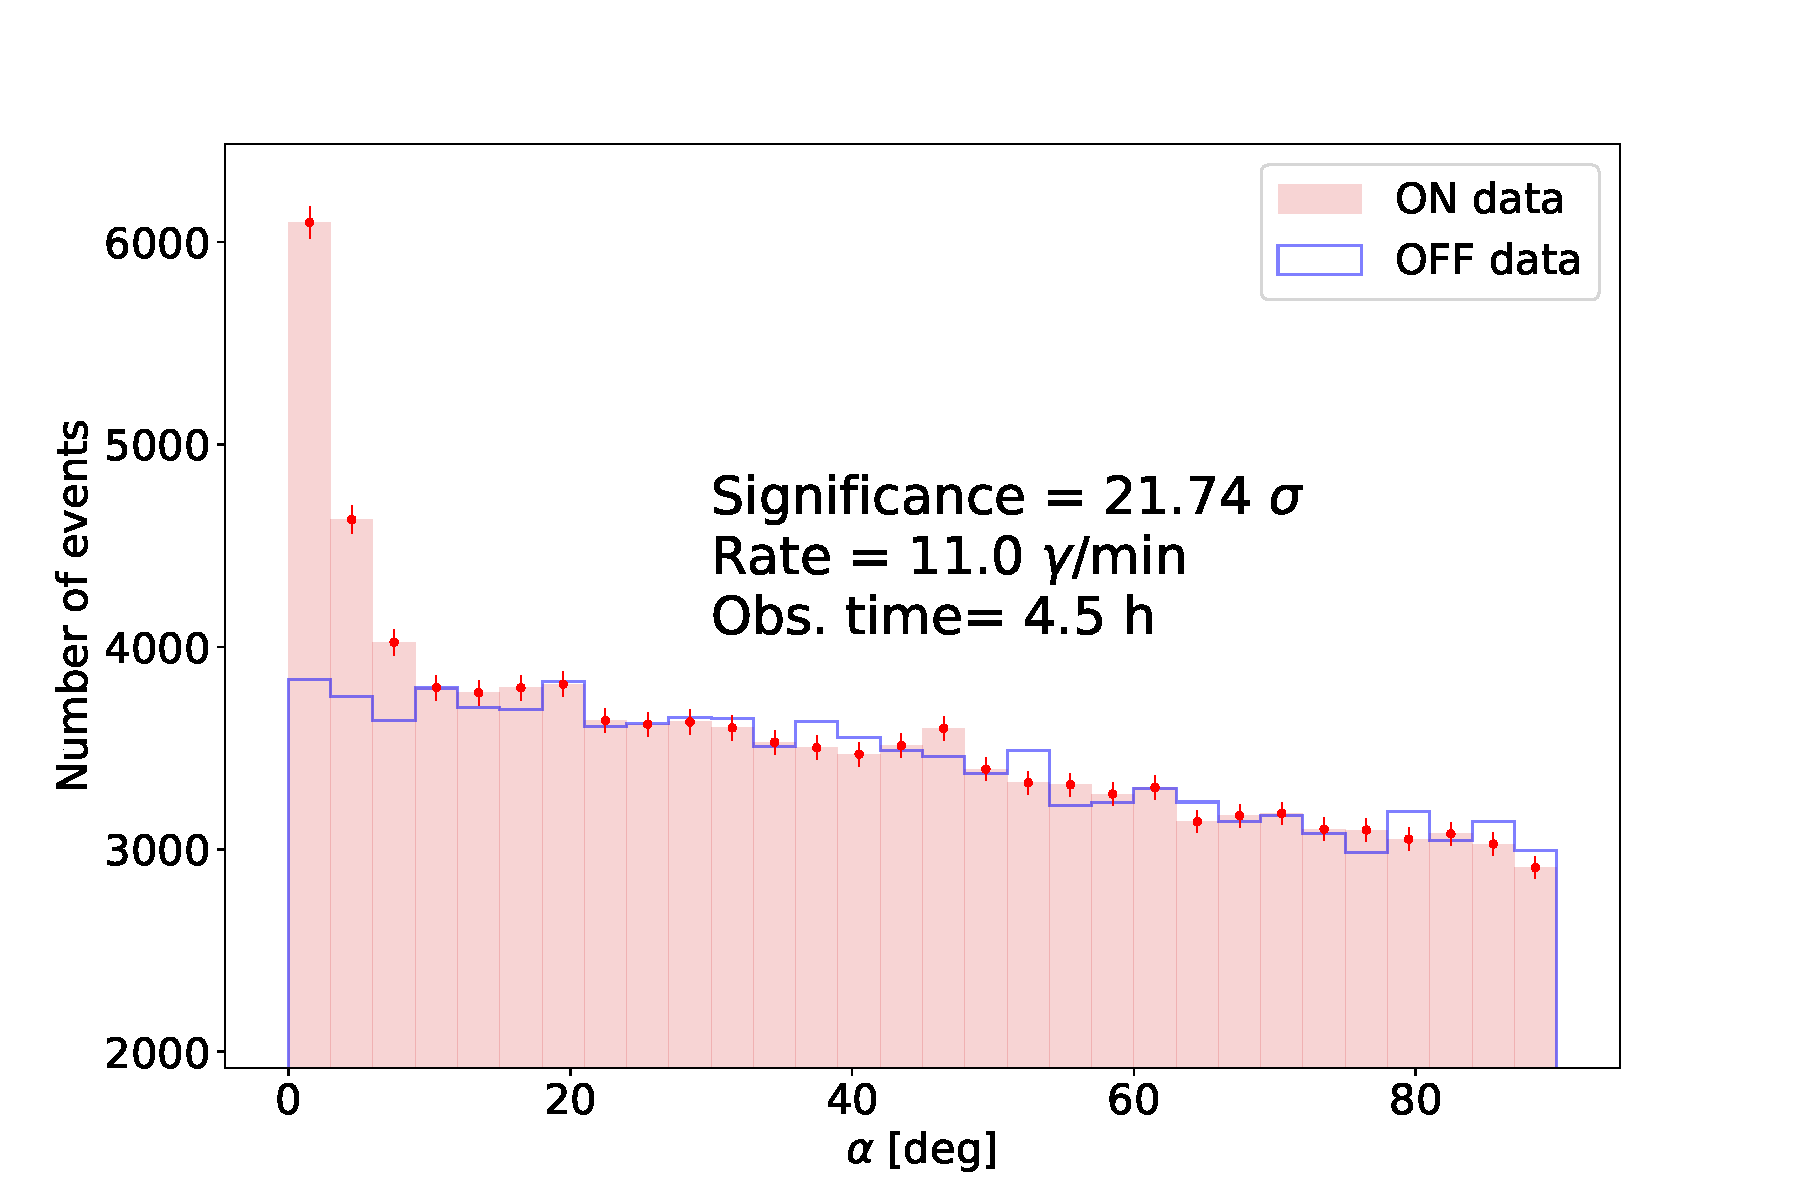
\includegraphics[width=\linewidth]{{Pictures/alphaplot_1stCrabCampaign_int100_gammaness0.60}.pdf}
    \caption{\small Intensity > 100, gammaness > 0.6} \label{fig:1st-b}
  \end{subfigure}
  \hspace*{\fill} % separation between the subfigures
  \begin{subfigure}{0.32\textwidth}
    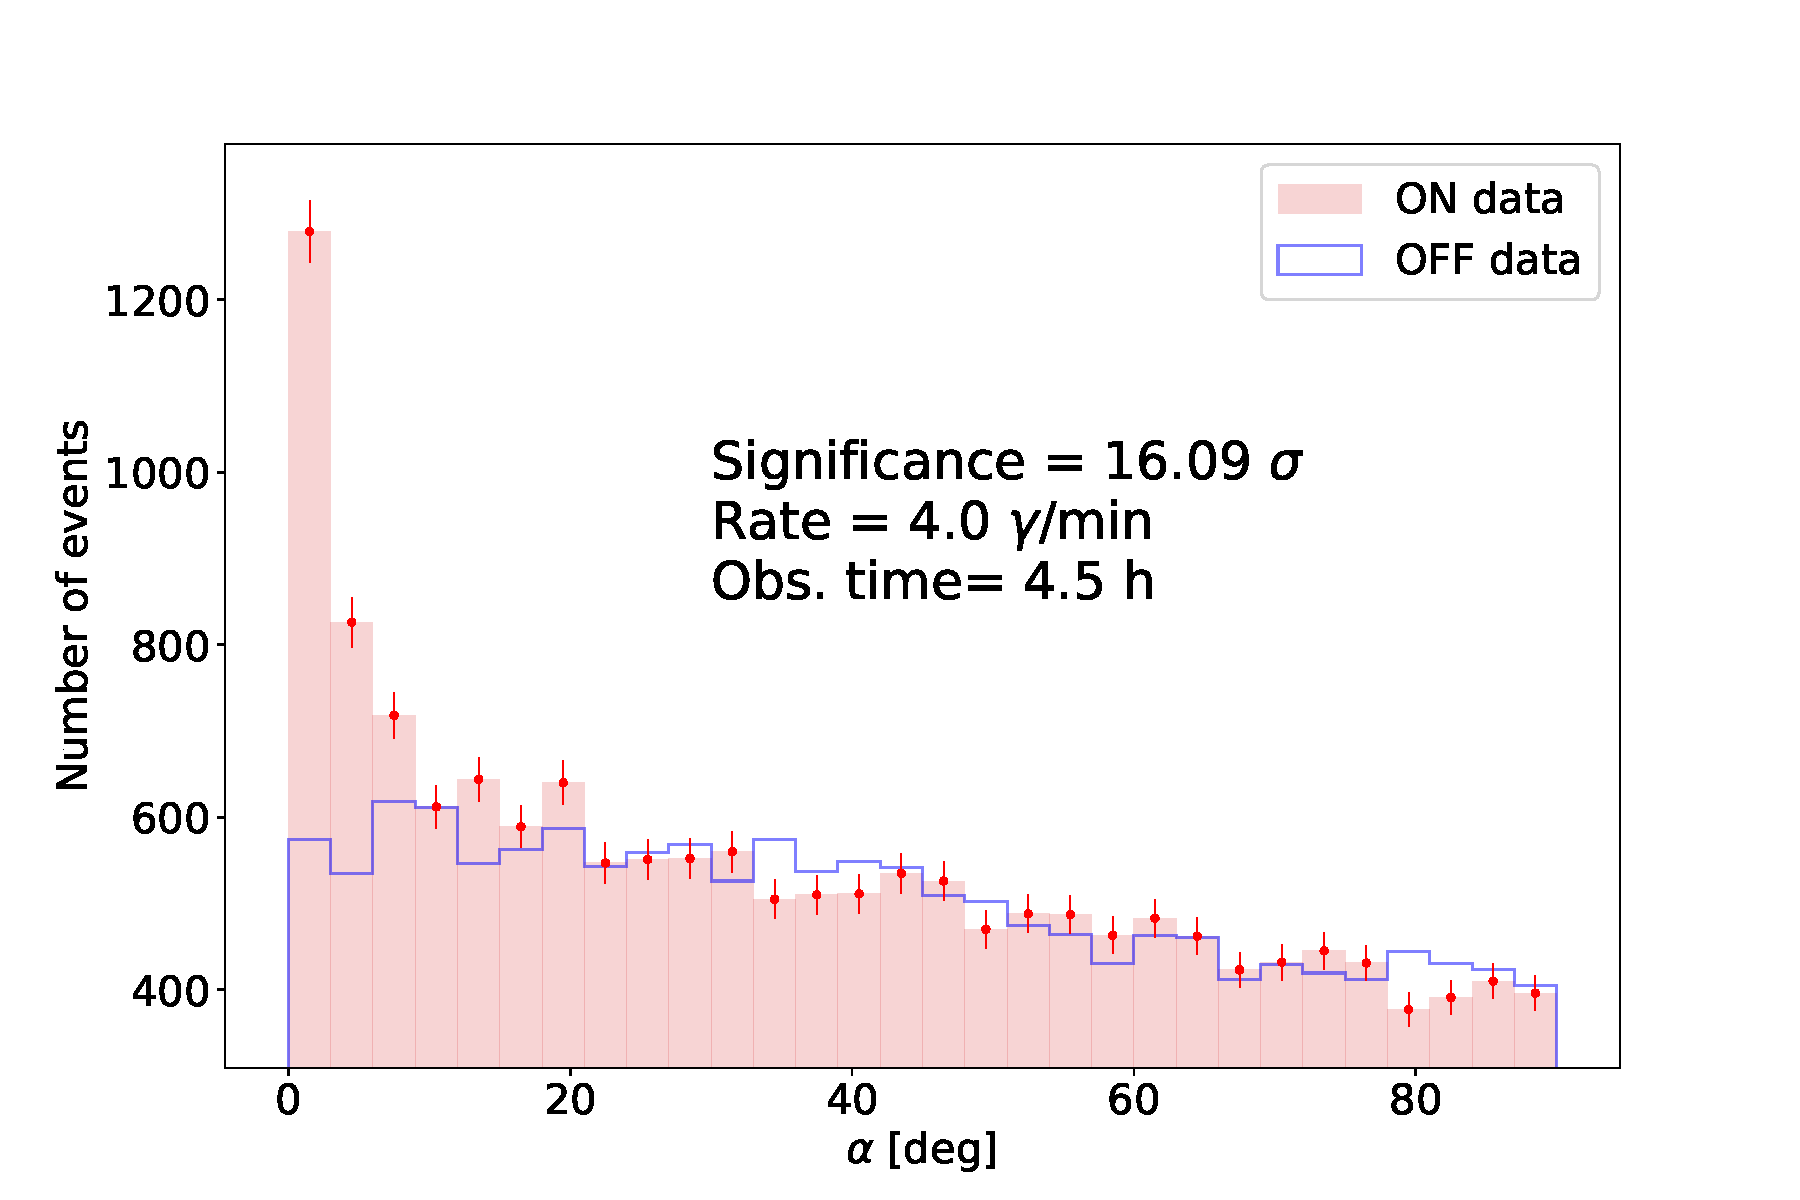
\includegraphics[width=\linewidth]{{Pictures/alphaplot_1stCrabCampaign_int100_gammaness0.70}.pdf}
    \caption{\small Intensity > 100, gammaness > 0.7} \label{fig:1st-c}
  \end{subfigure} \\
  \begin{subfigure}{0.32\textwidth}
    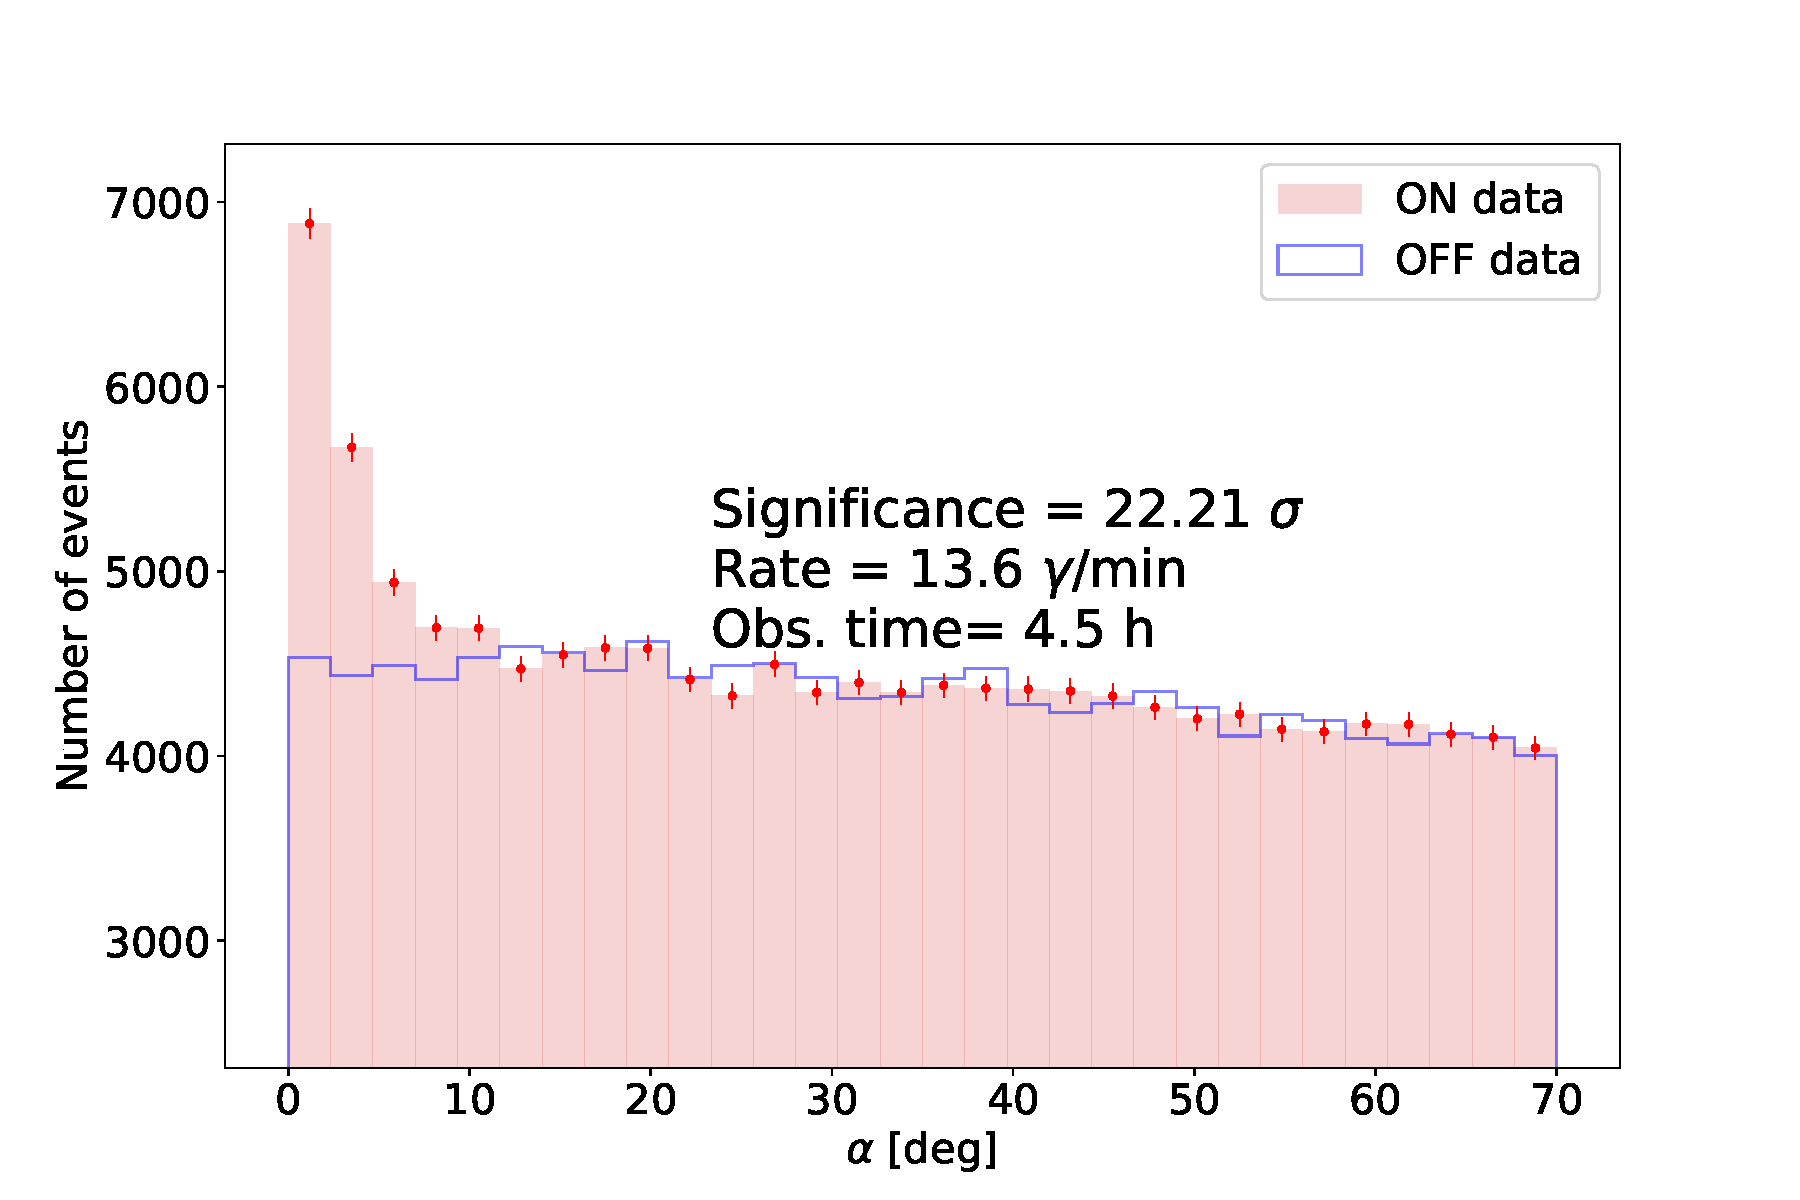
\includegraphics[width=\linewidth]{{Pictures/alphaplot_1stCrabCampaign_int500_gammaness0.50}.pdf}
    \caption{\small Intensity > 500, gammaness > 0.5} \label{fig:1st-d}
  \end{subfigure}
  \hspace*{\fill} % separation between the subfigures
  \begin{subfigure}{0.32\textwidth}
    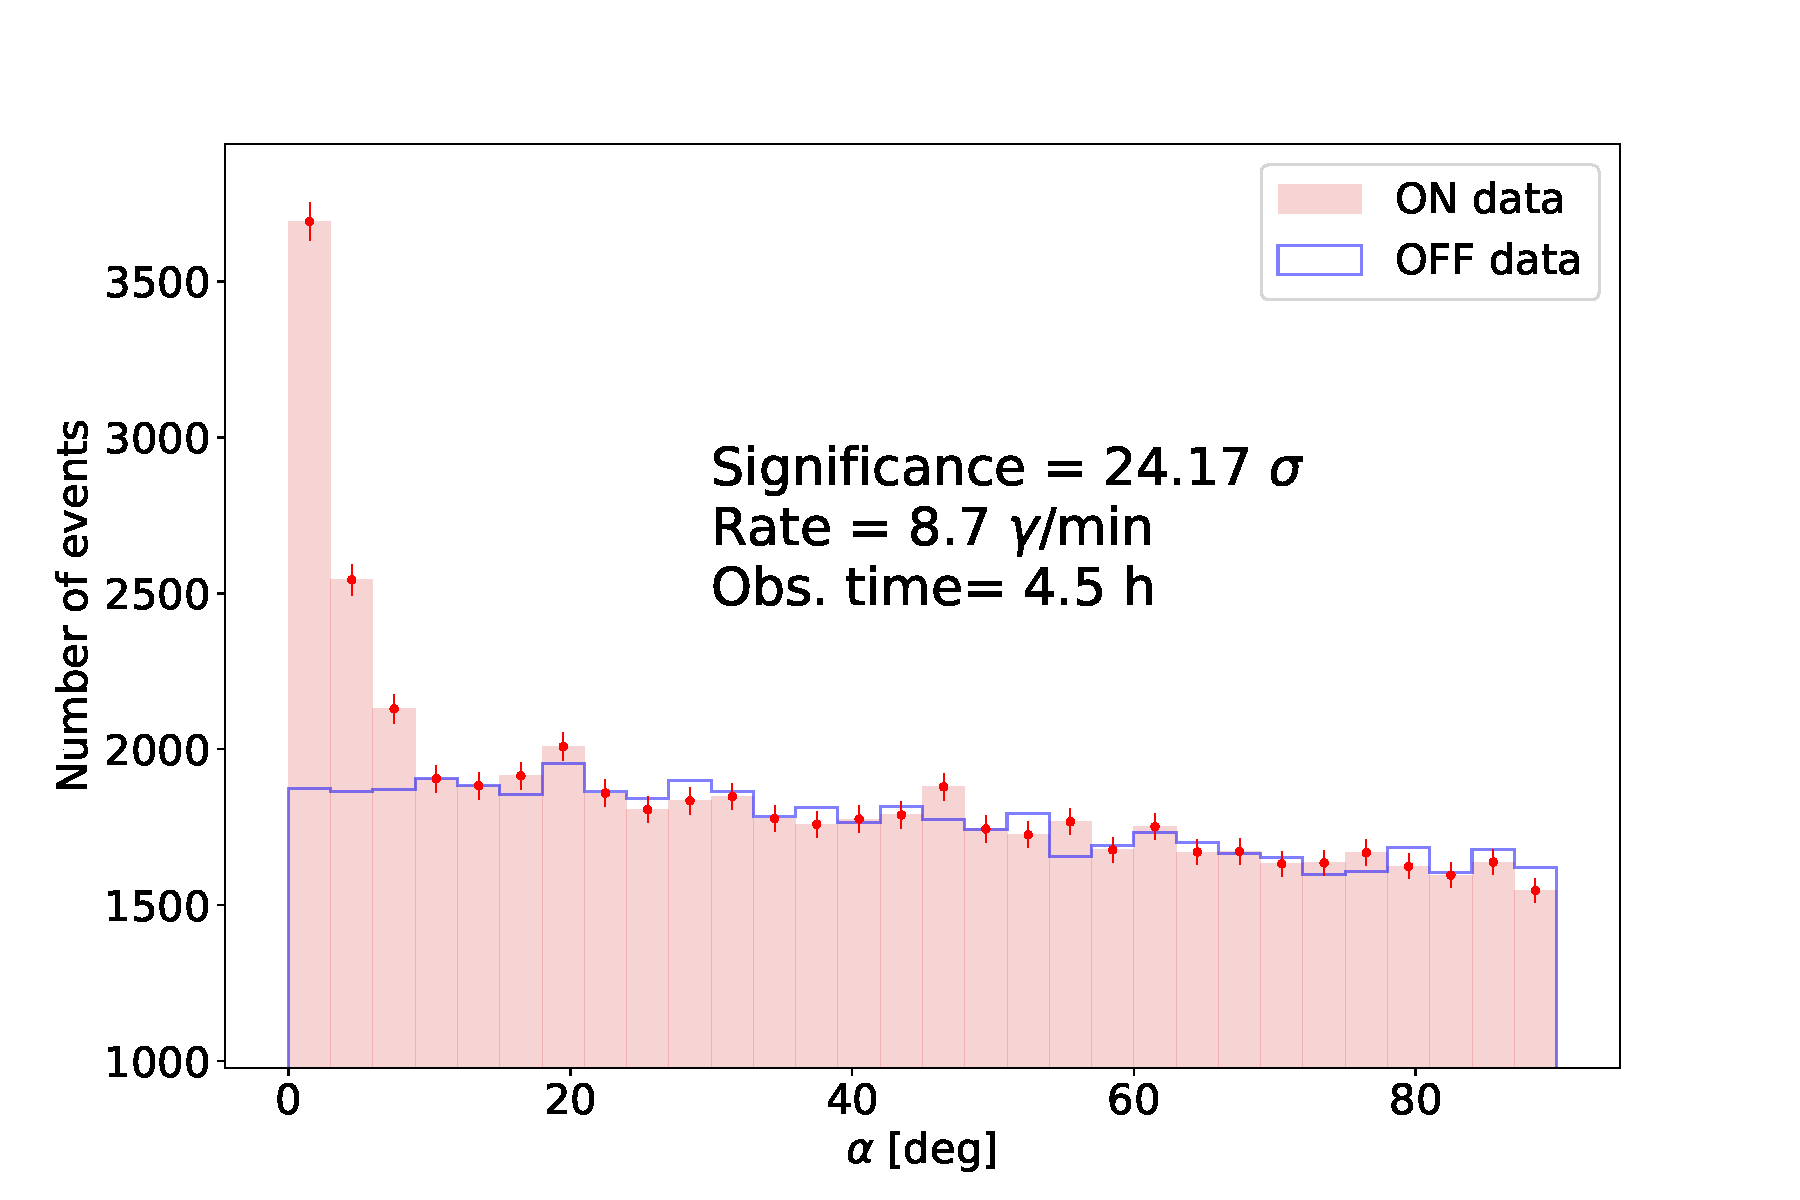
\includegraphics[width=\linewidth]{{Pictures/alphaplot_1stCrabCampaign_int500_gammaness0.60}.pdf}
    \caption{\small Intensity > 500, gammaness > 0.6} \label{fig:1st-e}
  \end{subfigure}
  \hspace*{\fill} % separation between the subfigures
  \begin{subfigure}{0.32\textwidth}
    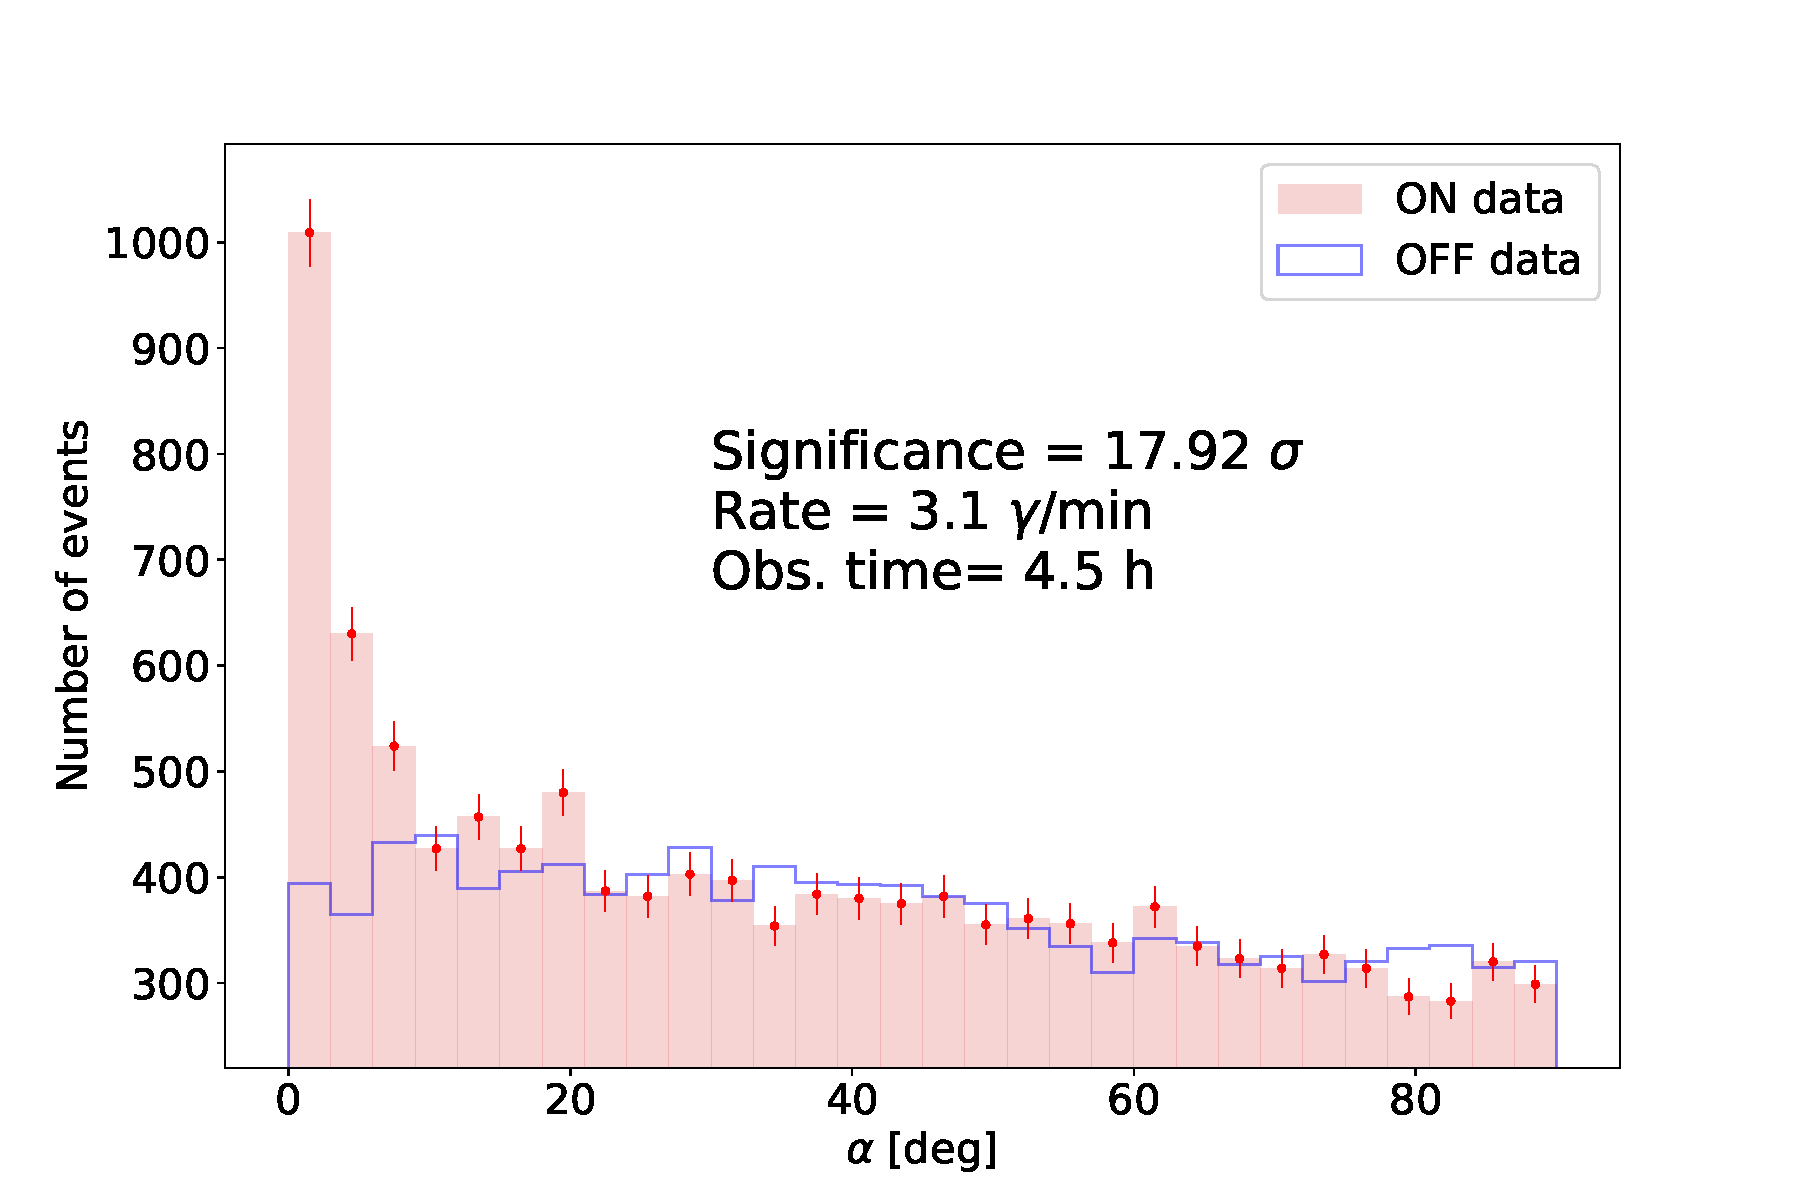
\includegraphics[width=\linewidth]{{Pictures/alphaplot_1stCrabCampaign_int500_gammaness0.70}.pdf}
    \caption{\small Intensity > 500, gammaness > 0.7} \label{fig:1st-f}
  \end{subfigure}
  \\
  \begin{subfigure}{0.32\textwidth}
    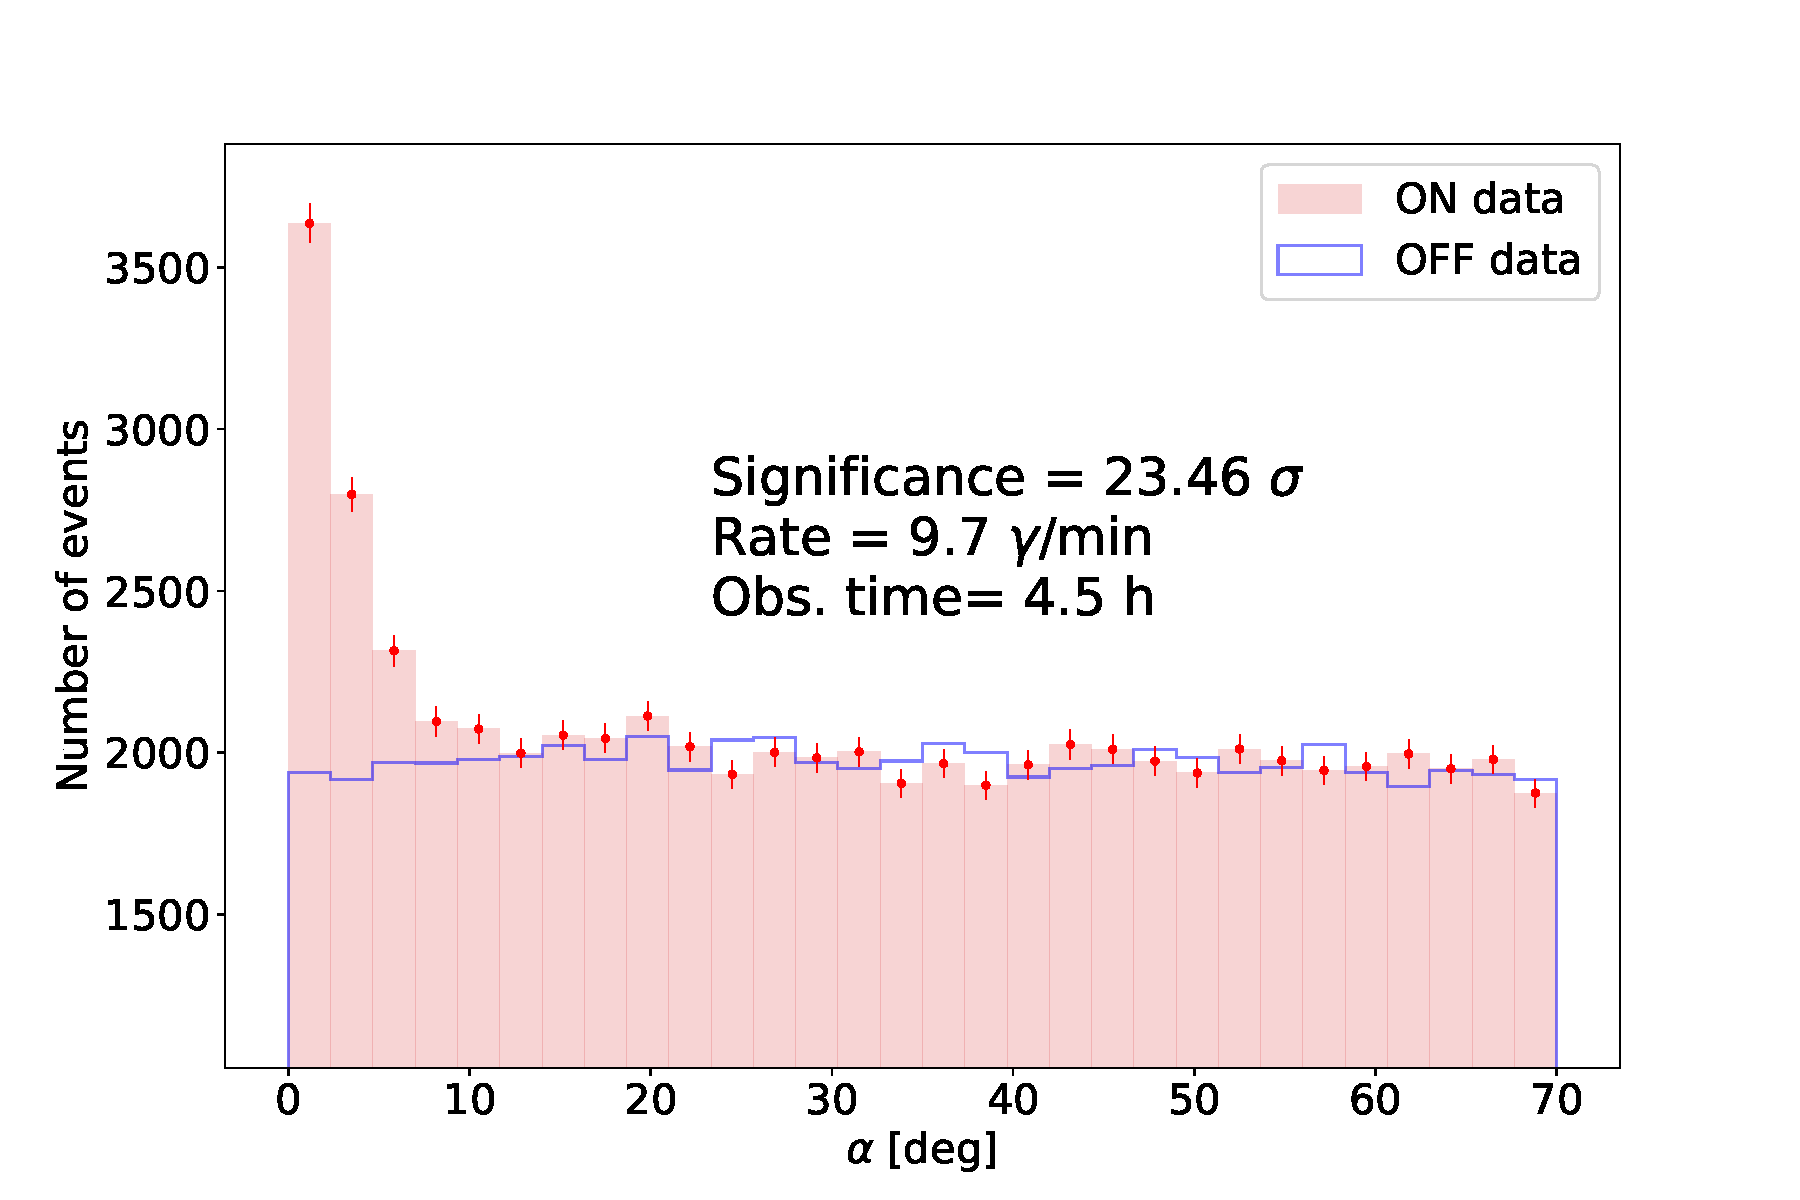
\includegraphics[width=\linewidth]{{Pictures/alphaplot_1stCrabCampaign_int1000_gammaness0.50}.pdf}
    \caption{\small Intensity > 1000, gammaness > 0.5} \label{fig:1st-g}
  \end{subfigure}
  \hspace*{\fill} % separation between the subfigures
  \begin{subfigure}{0.32\textwidth}
    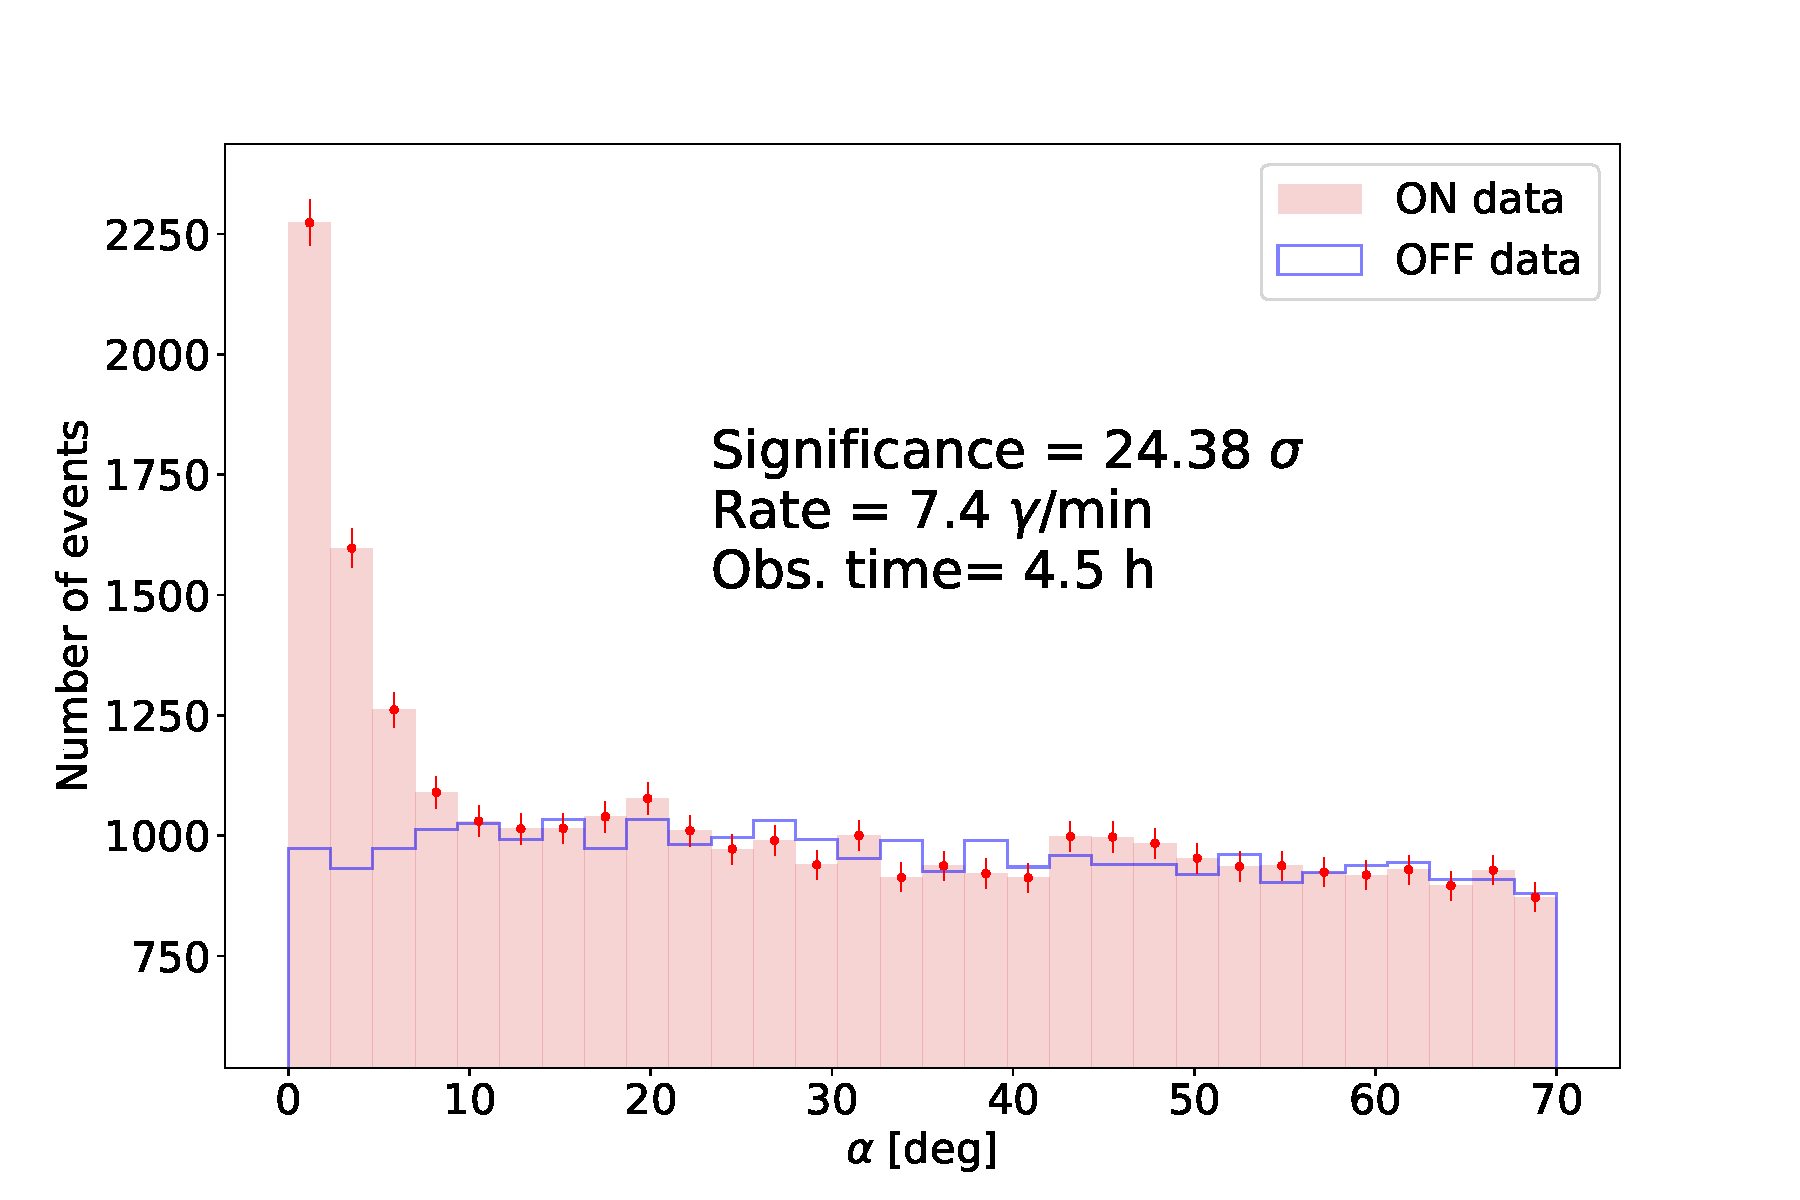
\includegraphics[width=\linewidth]{{Pictures/alphaplot_1stCrabCampaign_int1000_gammaness0.60}.pdf}
    \caption{\small Intensity > 1000, gammaness > 0.6} \label{fig:1st-h}
  \end{subfigure}
  \hspace*{\fill} % separation between the subfigures
  \begin{subfigure}{0.32\textwidth}
    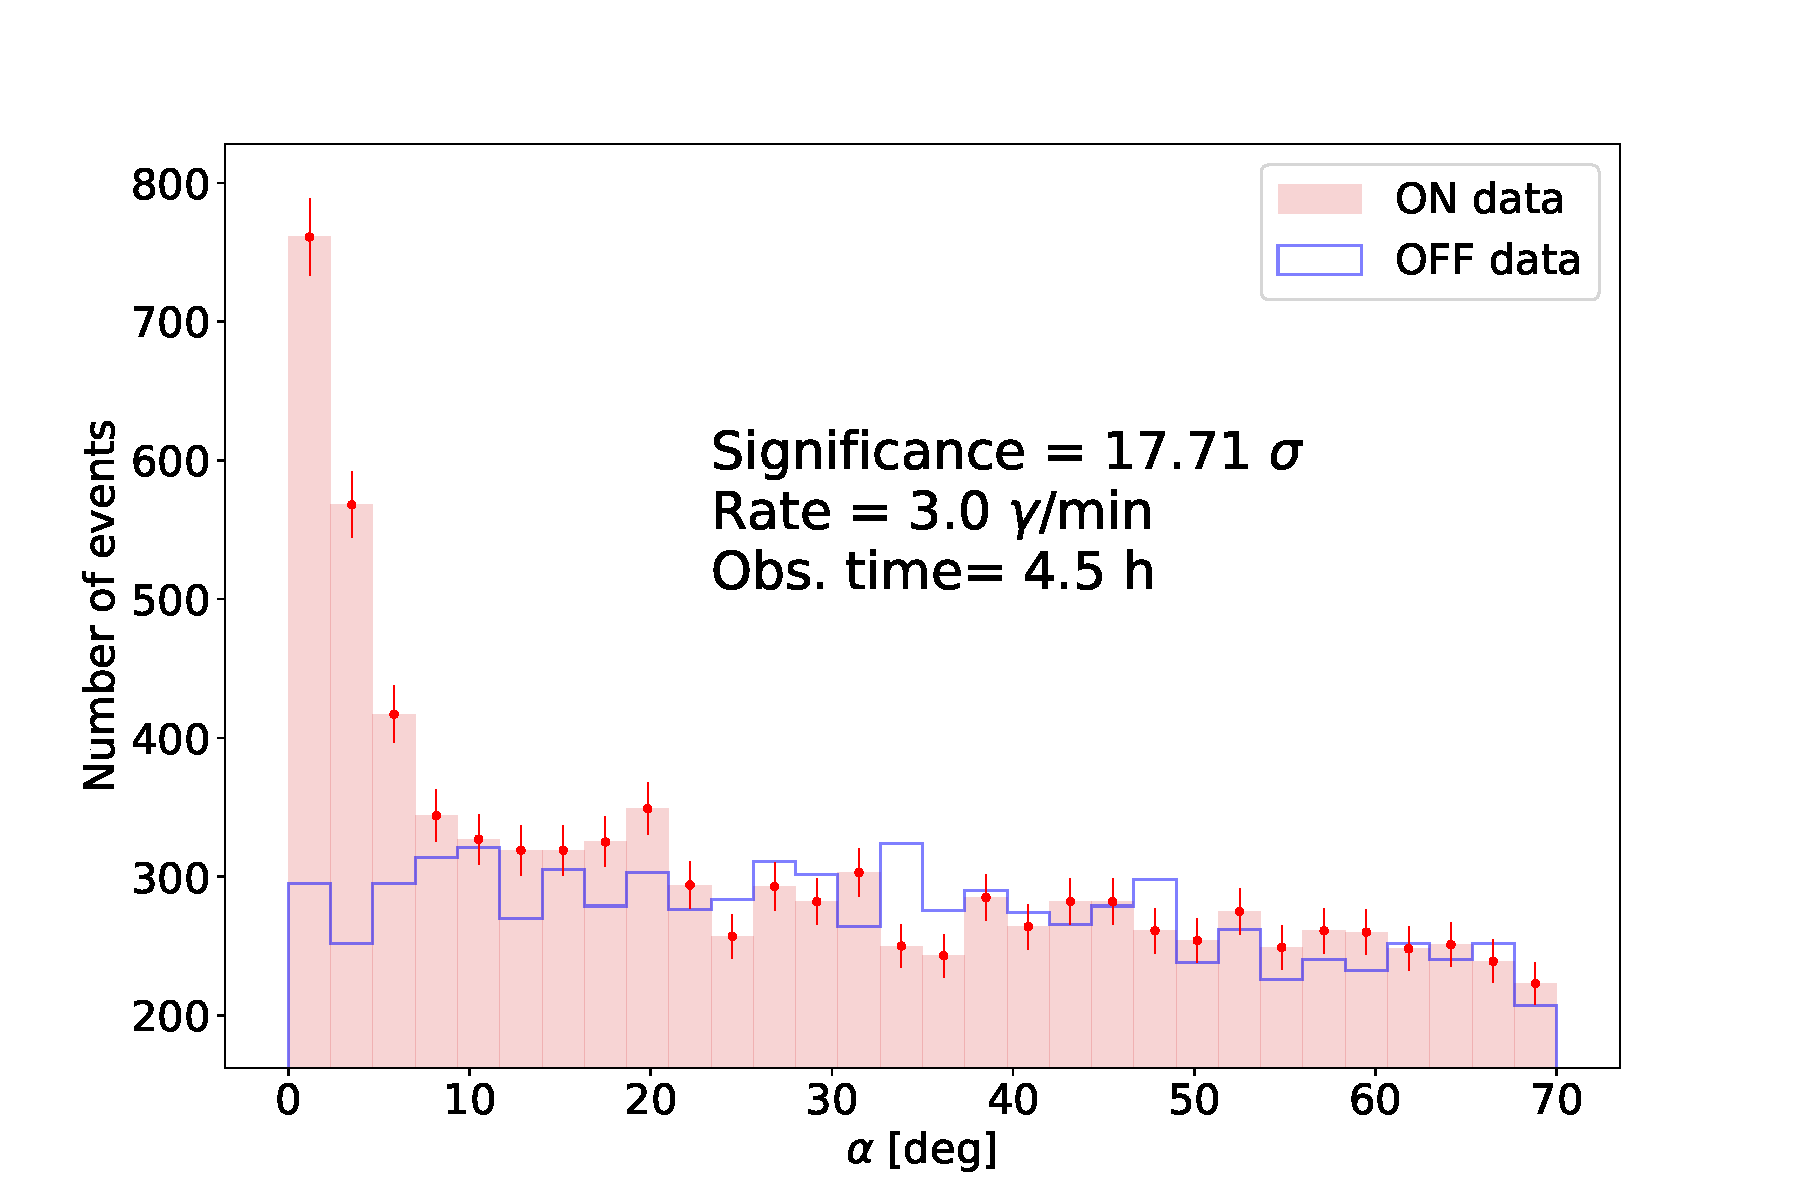
\includegraphics[width=\linewidth]{{Pictures/alphaplot_1stCrabCampaign_int1000_gammaness0.70}.pdf}
    \caption{\small Intensity > 1000, gammaness > 0.7} \label{fig:1st-i}
  \end{subfigure}
  \caption{Results of $\alpha$ plot of the First Crab Campaign of \gls{lst} for different cuts in intensity and gammaness. In each plot the reached significance is shown, defined as explained in section \ref{sec:realdata}, together with the rate of $\gamma$s per minute and the total observation time. \label{fig:1st-crab-campaign}}
\end{figure}

\begin{figure}[h]
  \begin{subfigure}{0.32\textwidth}
    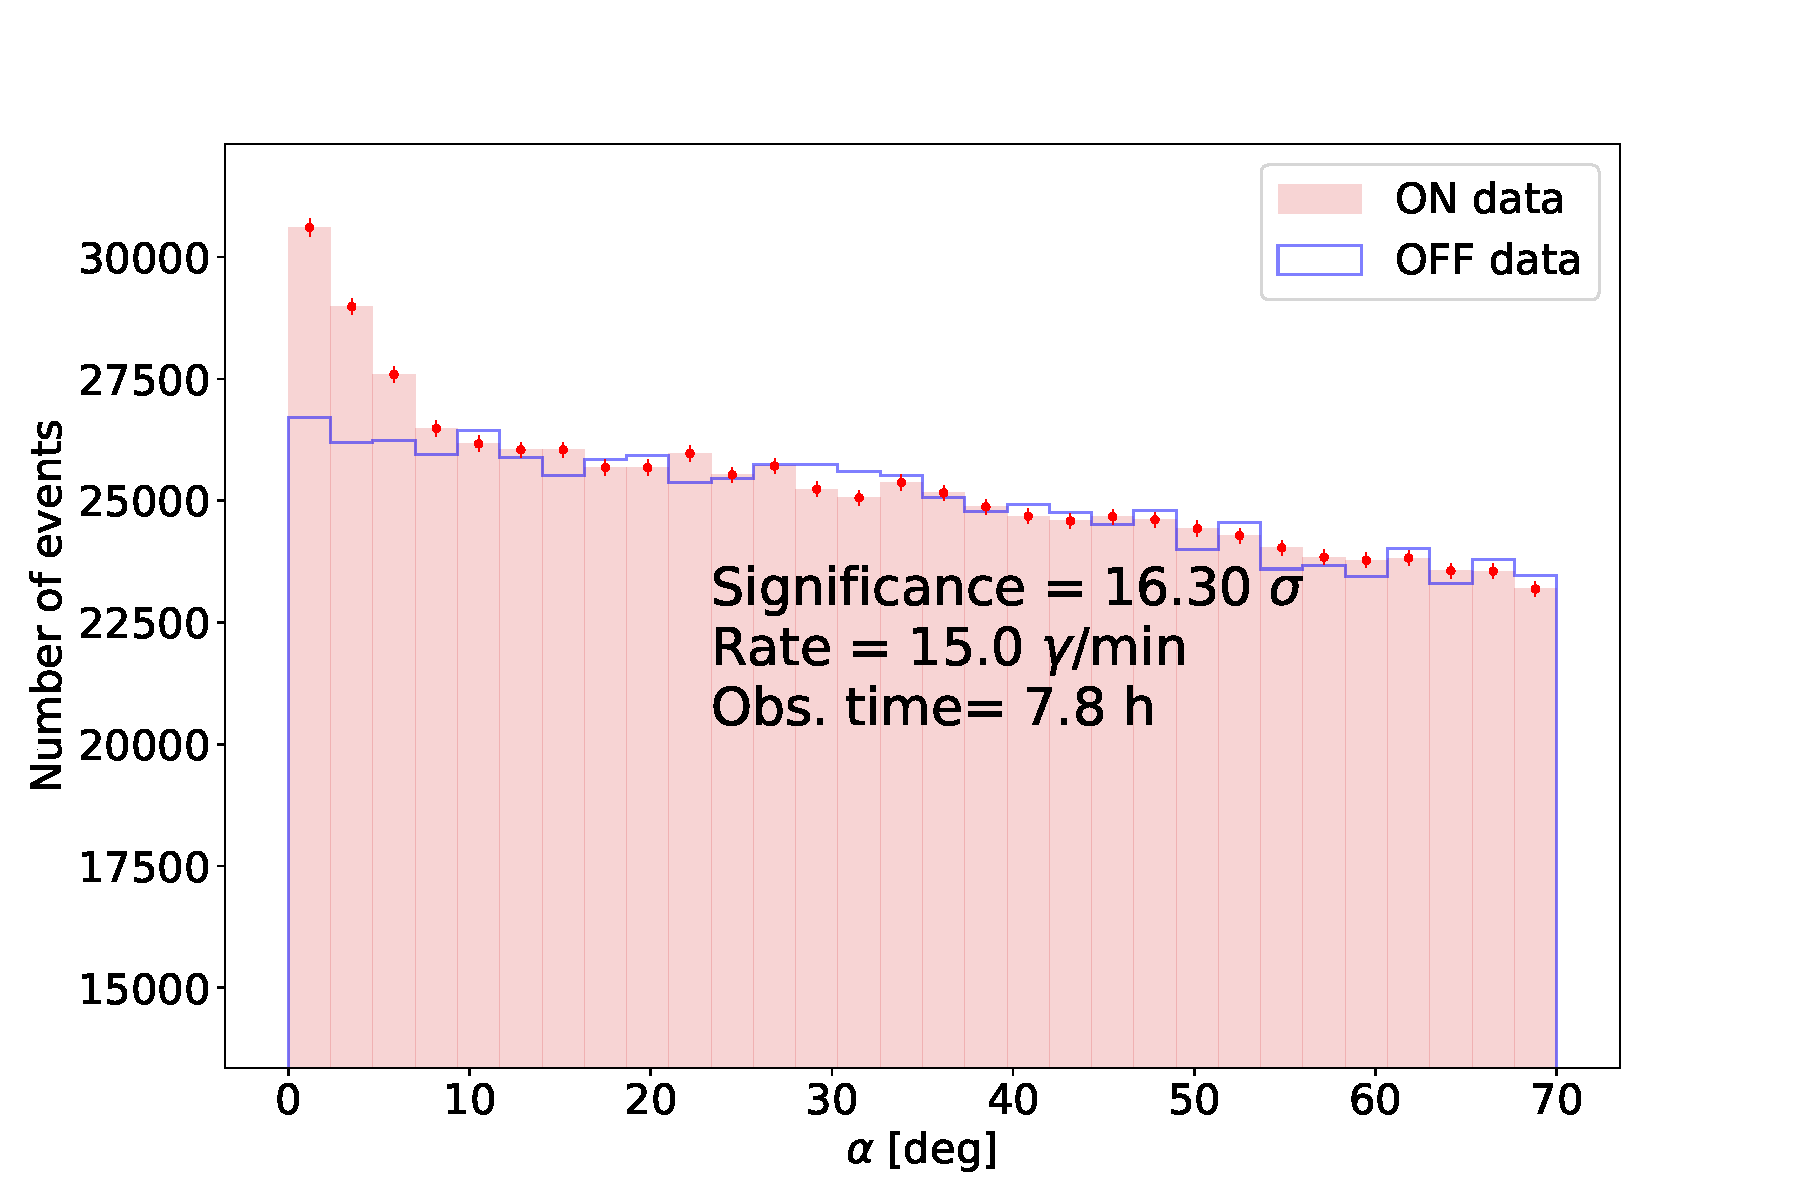
\includegraphics[width=\linewidth]{{Pictures/alphaplot_2ndCrabCampaign_int100_gammaness0.50}.pdf}
    \caption{\small Intensity > 100, gammaness > 0.5} \label{fig:2nd-a}
  \end{subfigure}
  \hspace*{\fill} % separation between the subfigures
  \begin{subfigure}{0.32\textwidth}
    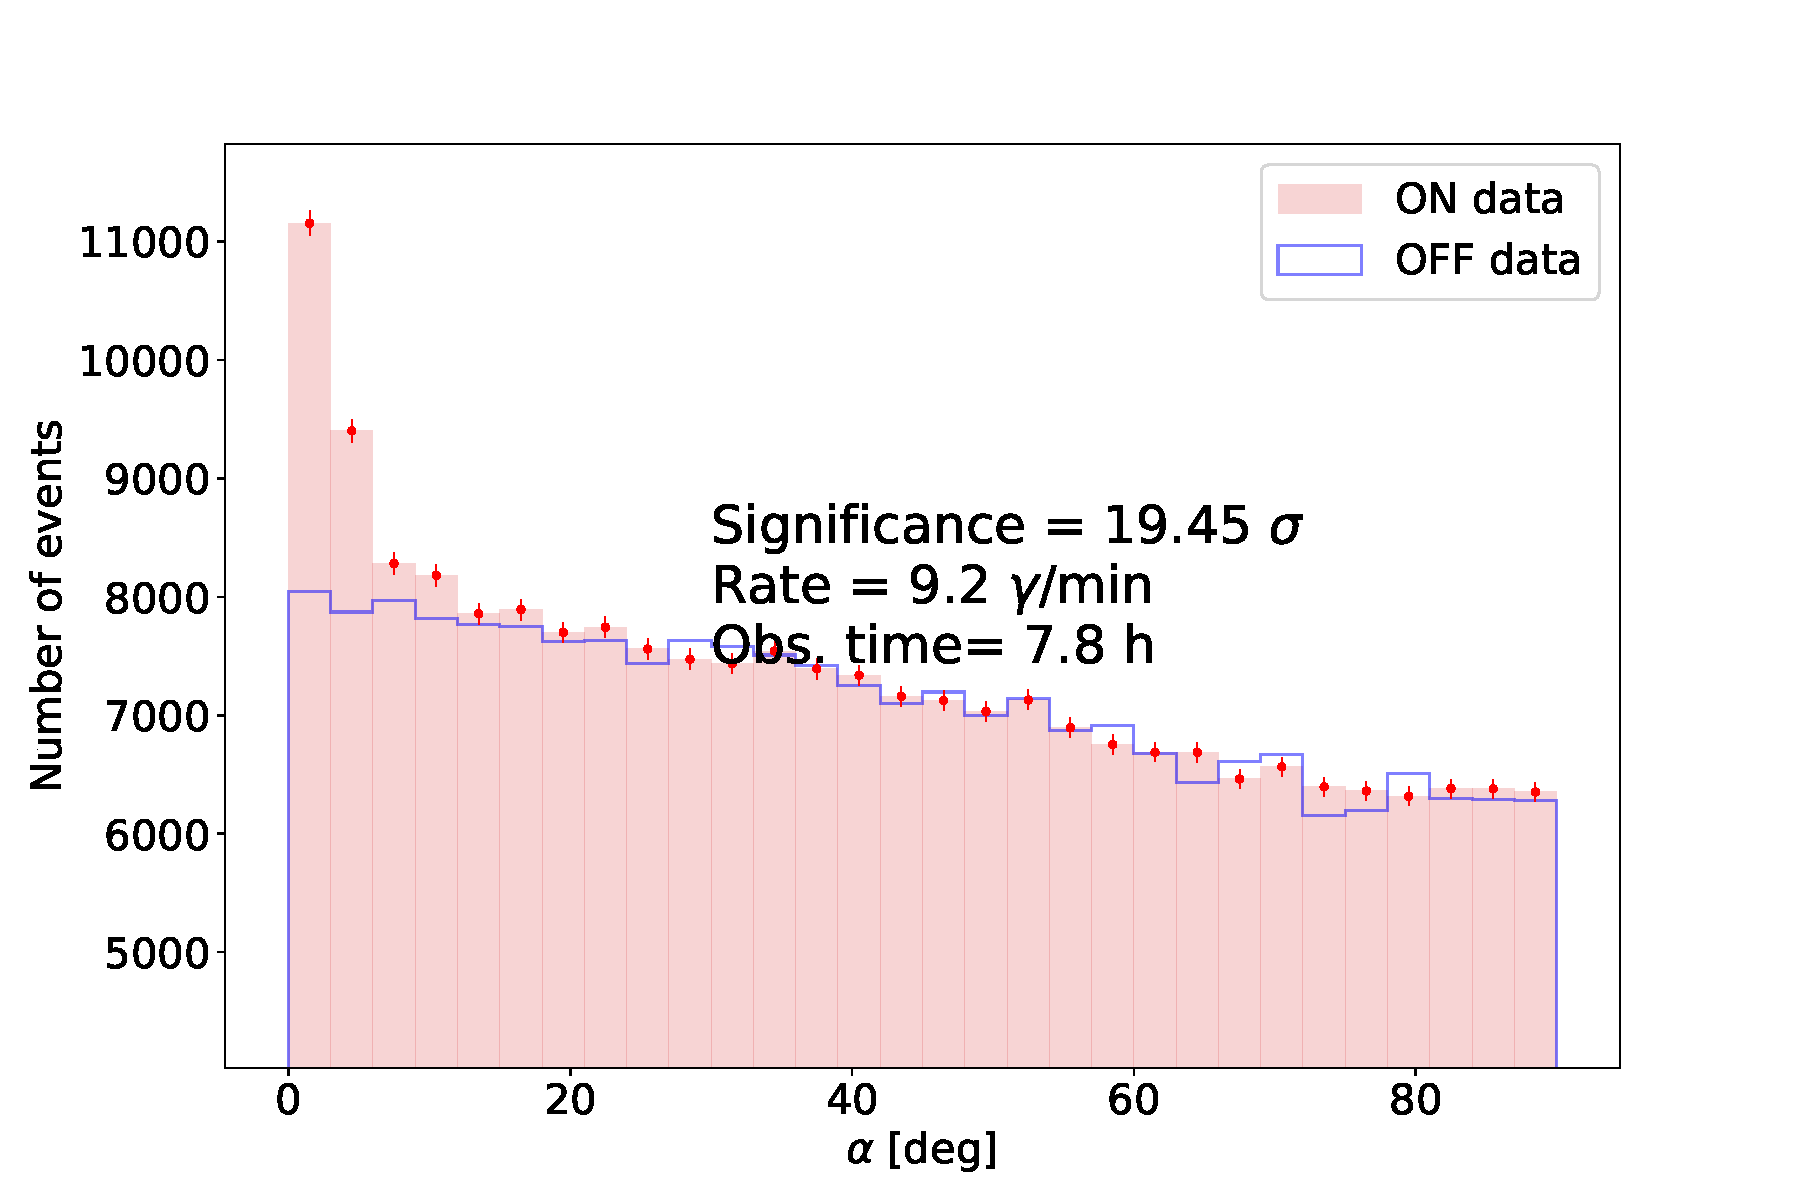
\includegraphics[width=\linewidth]{{Pictures/alphaplot_2ndCrabCampaign_int100_gammaness0.60}.pdf}
    \caption{\small Intensity > 100, gammaness > 0.6} \label{fig:2nd-b}
  \end{subfigure}
  \hspace*{\fill} % separation between the subfigures
  \begin{subfigure}{0.32\textwidth}
    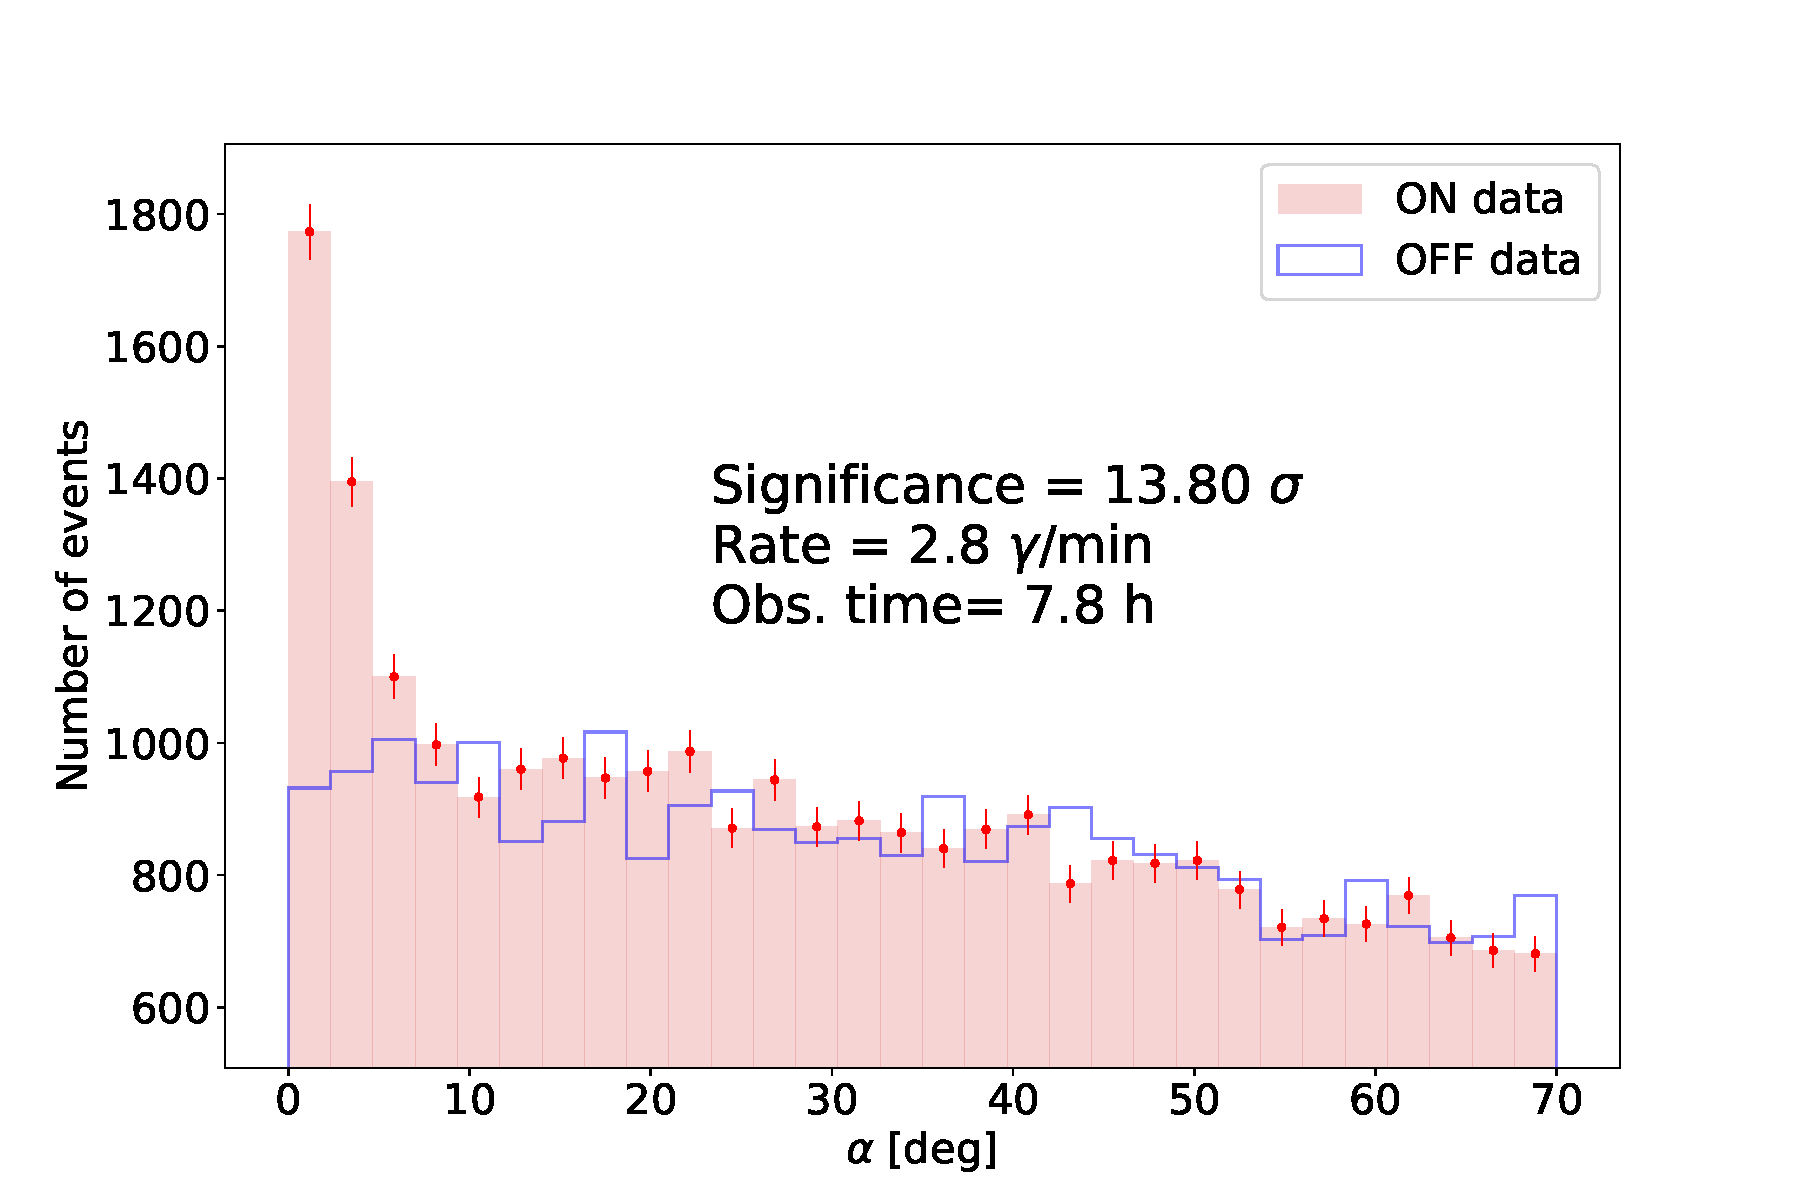
\includegraphics[width=\linewidth]{{Pictures/alphaplot_2ndCrabCampaign_int100_gammaness0.70}.pdf}
    \caption{\small Intensity > 100, gammaness > 0.7} \label{fig:2nd-c}
  \end{subfigure} \\
  \begin{subfigure}{0.32\textwidth}
    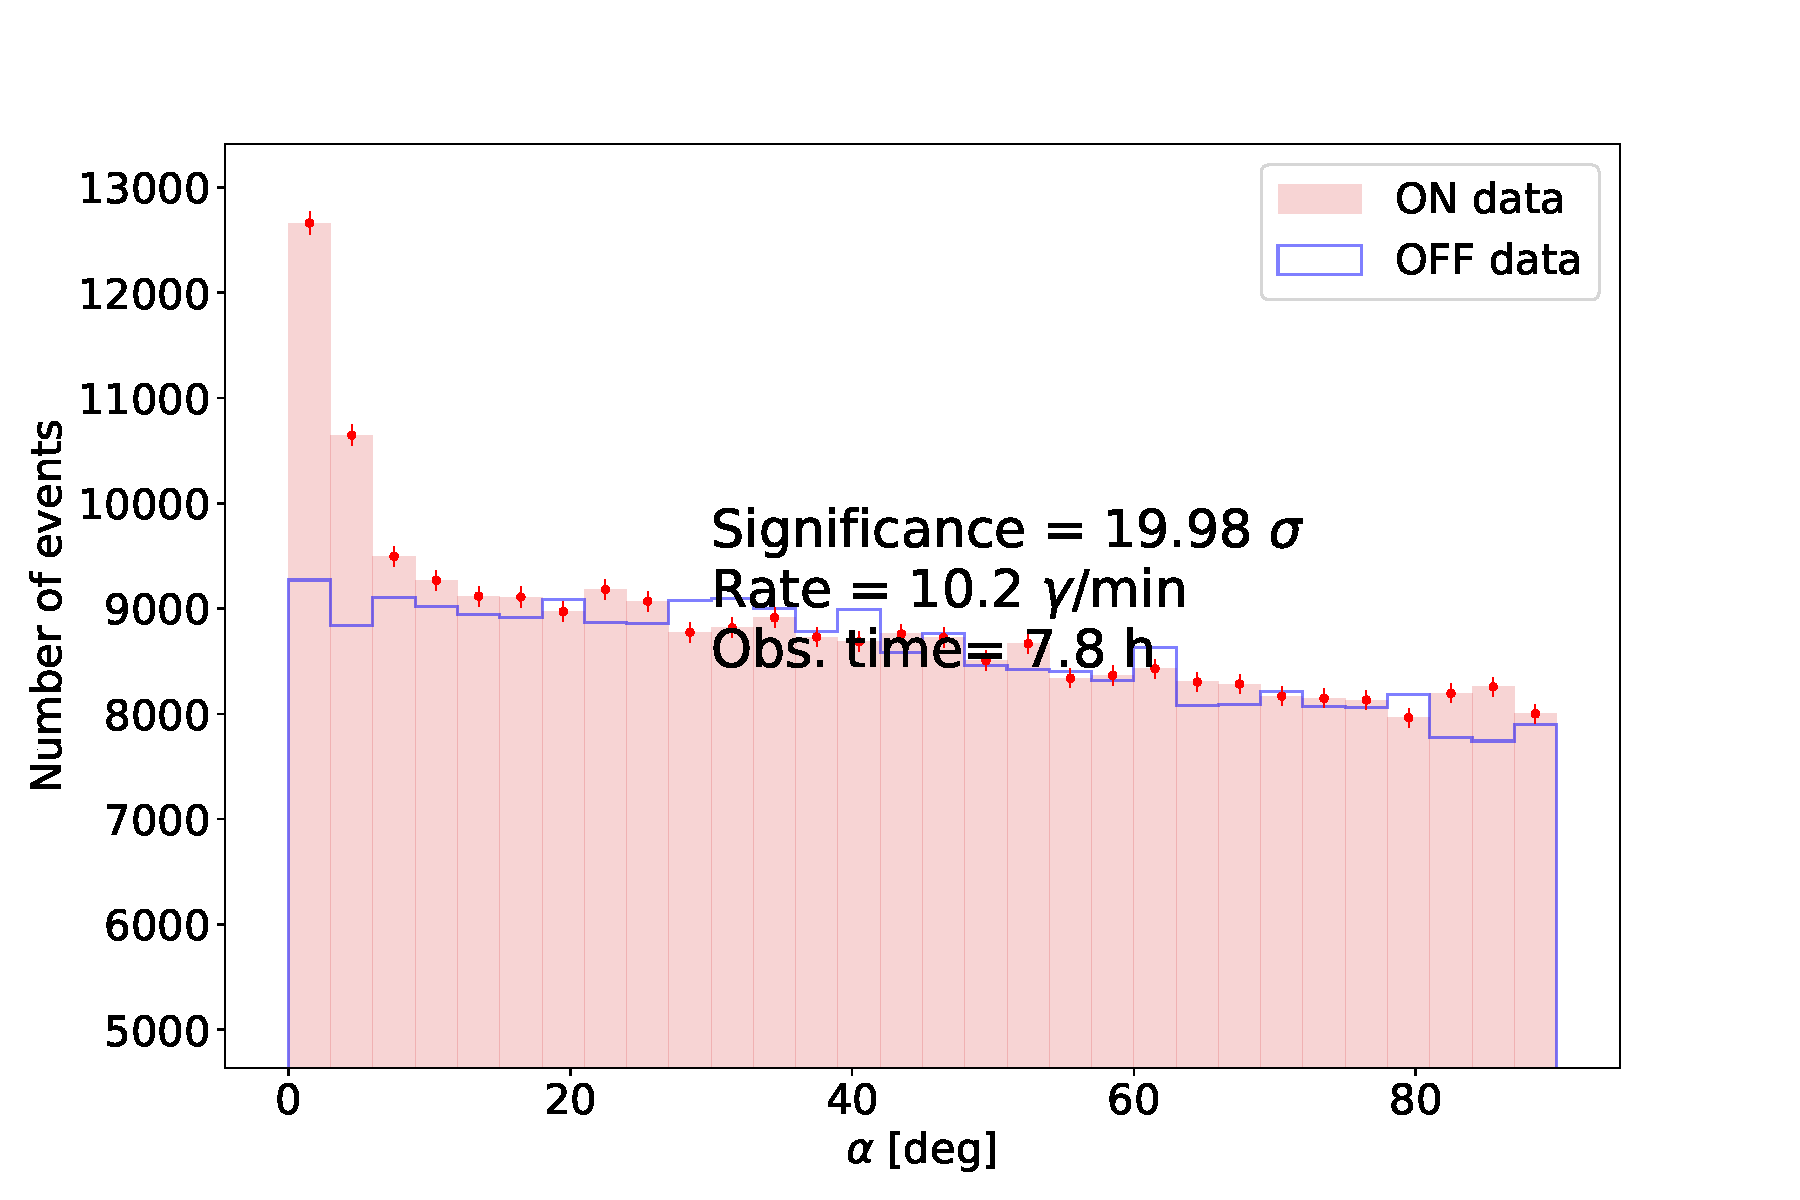
\includegraphics[width=\linewidth]{{Pictures/alphaplot_2ndCrabCampaign_int500_gammaness0.50}.pdf}
    \caption{\small Intensity > 500, gammaness > 0.5} \label{fig:2nd-d}
  \end{subfigure}
  \hspace*{\fill} % separation between the subfigures
  \begin{subfigure}{0.32\textwidth}
    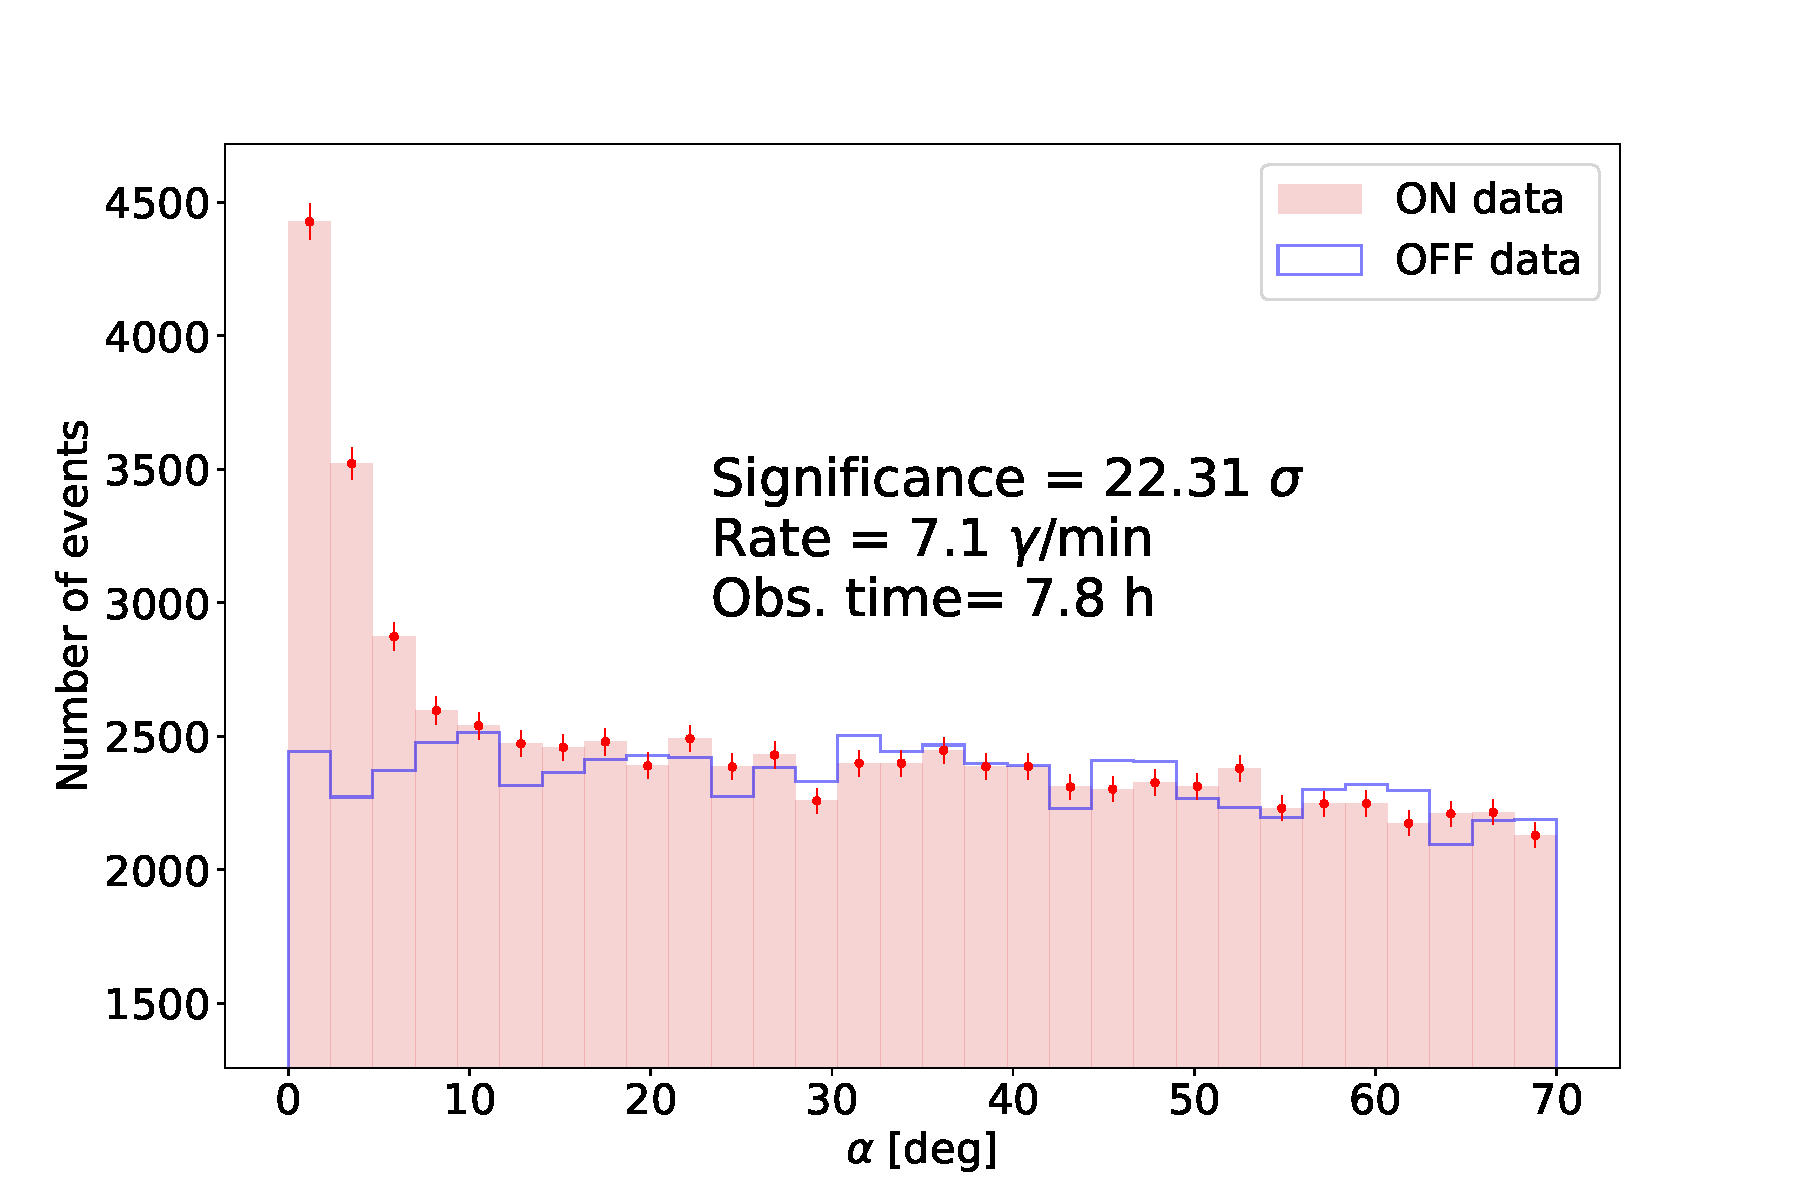
\includegraphics[width=\linewidth]{{Pictures/alphaplot_2ndCrabCampaign_int500_gammaness0.60}.pdf}
    \caption{\small Intensity > 500, gammaness > 0.6} \label{fig:2nd-e}
  \end{subfigure}
  \hspace*{\fill} % separation between the subfigures
  \begin{subfigure}{0.32\textwidth}
    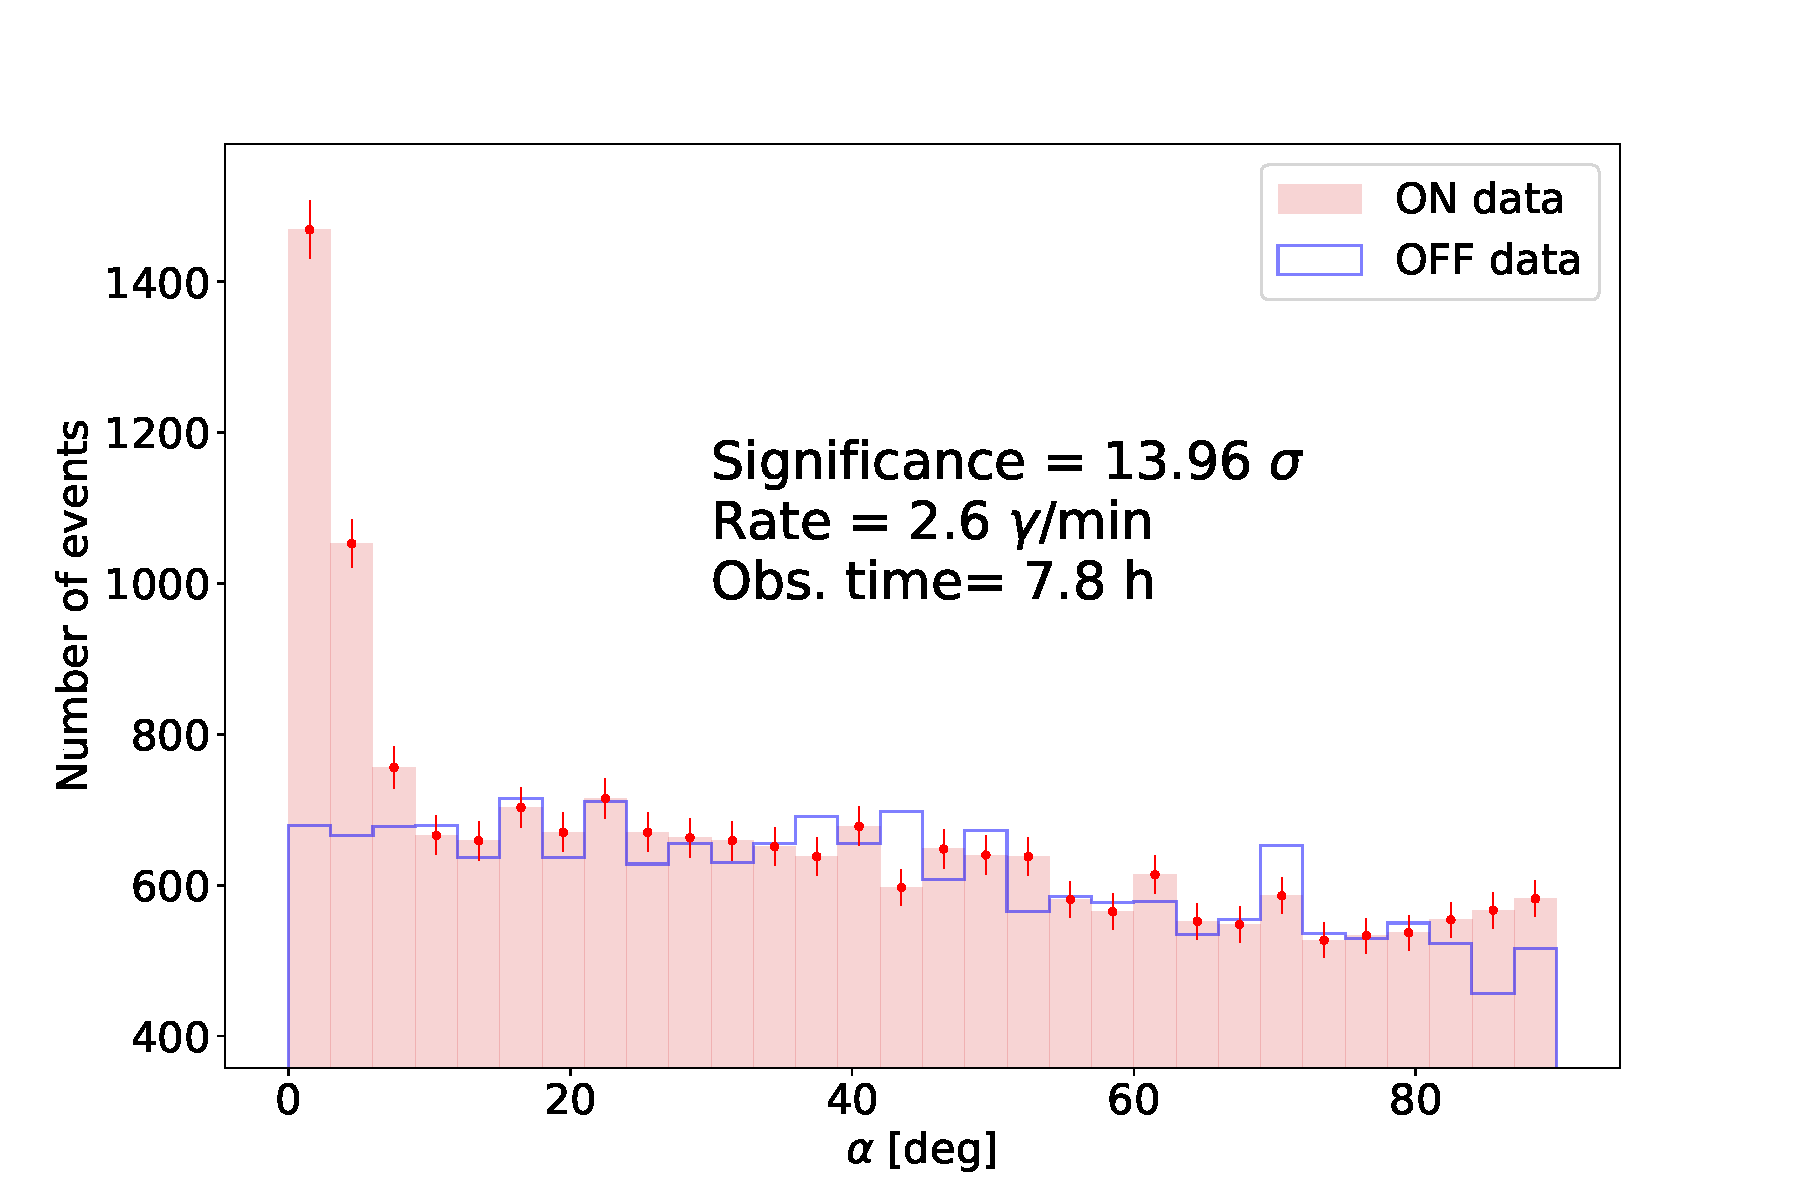
\includegraphics[width=\linewidth]{{Pictures/alphaplot_2ndCrabCampaign_int500_gammaness0.70}.pdf}
    \caption{\small Intensity > 500, gammaness > 0.7} \label{fig:2nd-f}
  \end{subfigure}
  \\
  \begin{subfigure}{0.32\textwidth}
    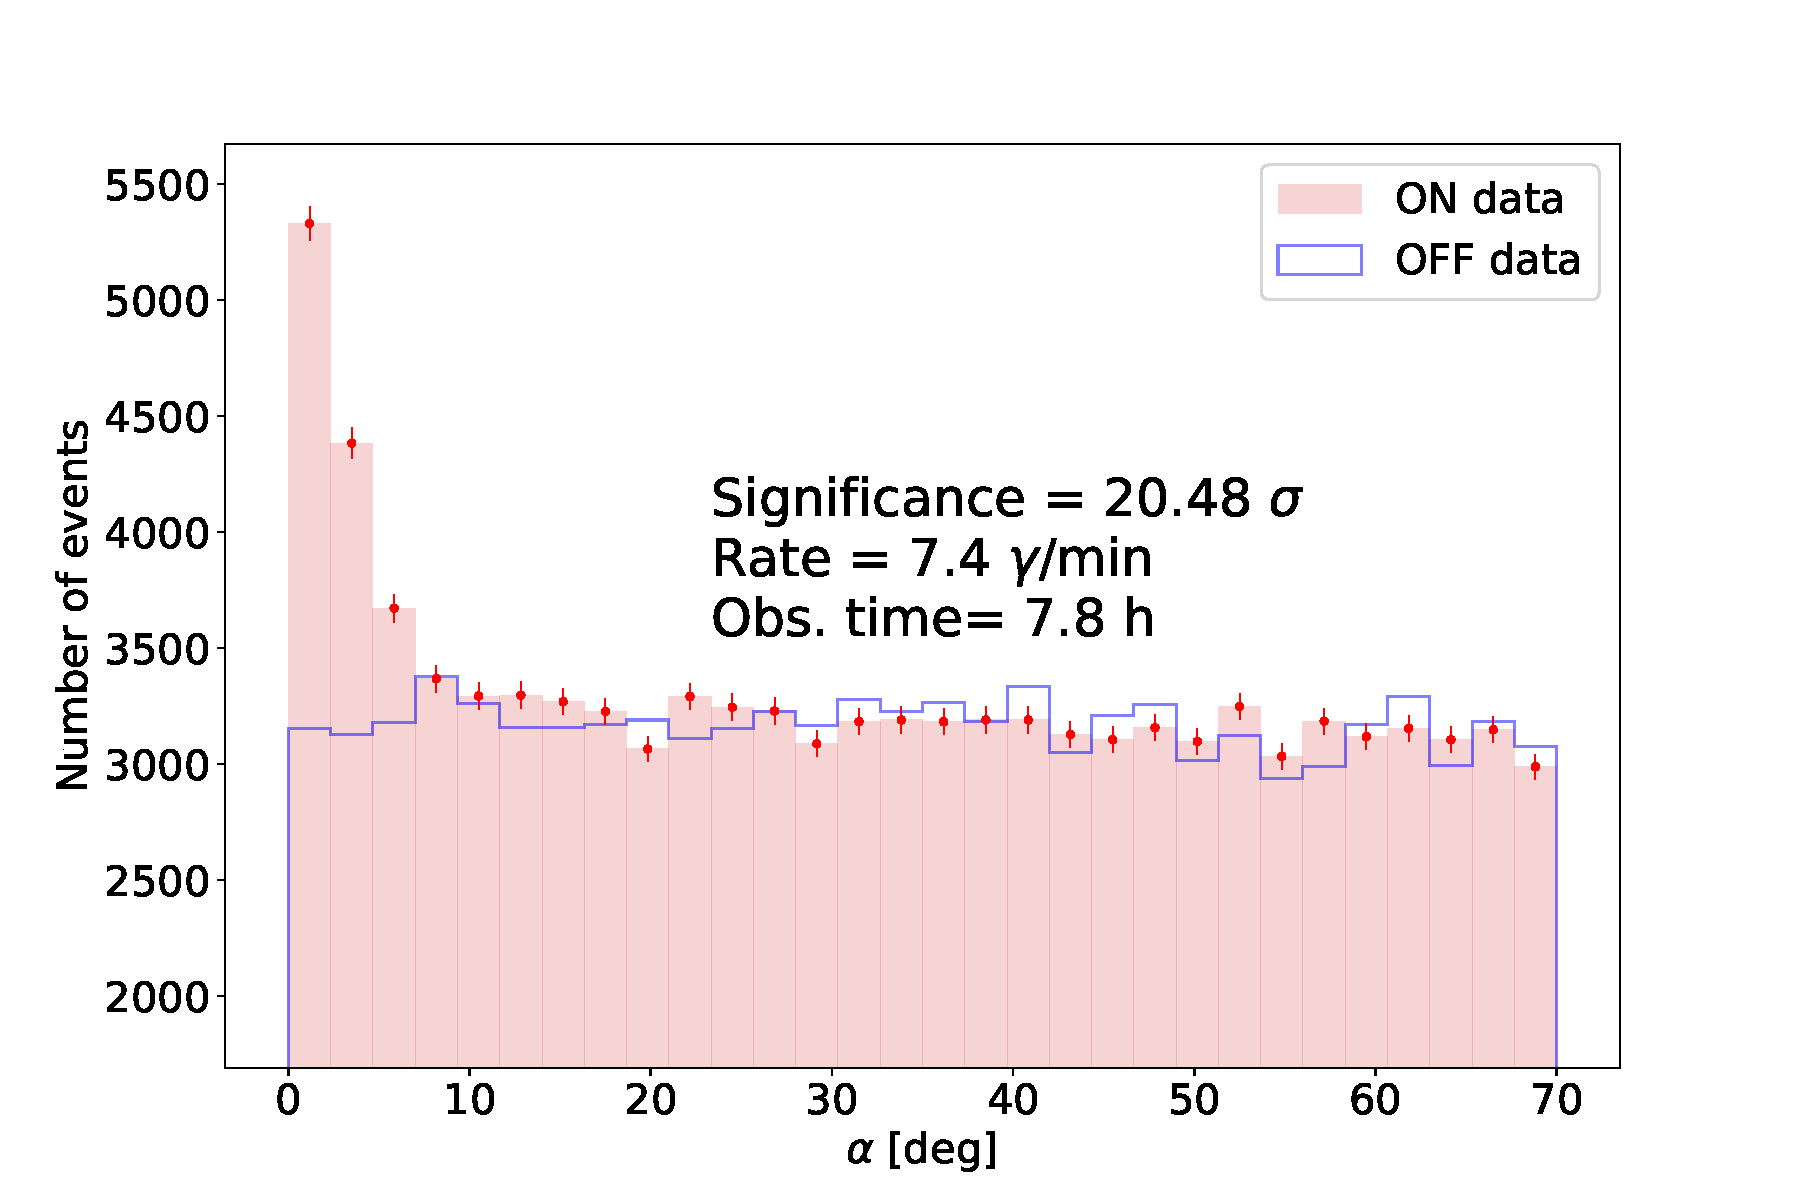
\includegraphics[width=\linewidth]{{Pictures/alphaplot_2ndCrabCampaign_int1000_gammaness0.50}.pdf}
    \caption{\small Intensity > 1000, gammaness > 0.5} \label{fig:2nd-g}
  \end{subfigure}
  \hspace*{\fill} % separation between the subfigures
  \begin{subfigure}{0.32\textwidth}
    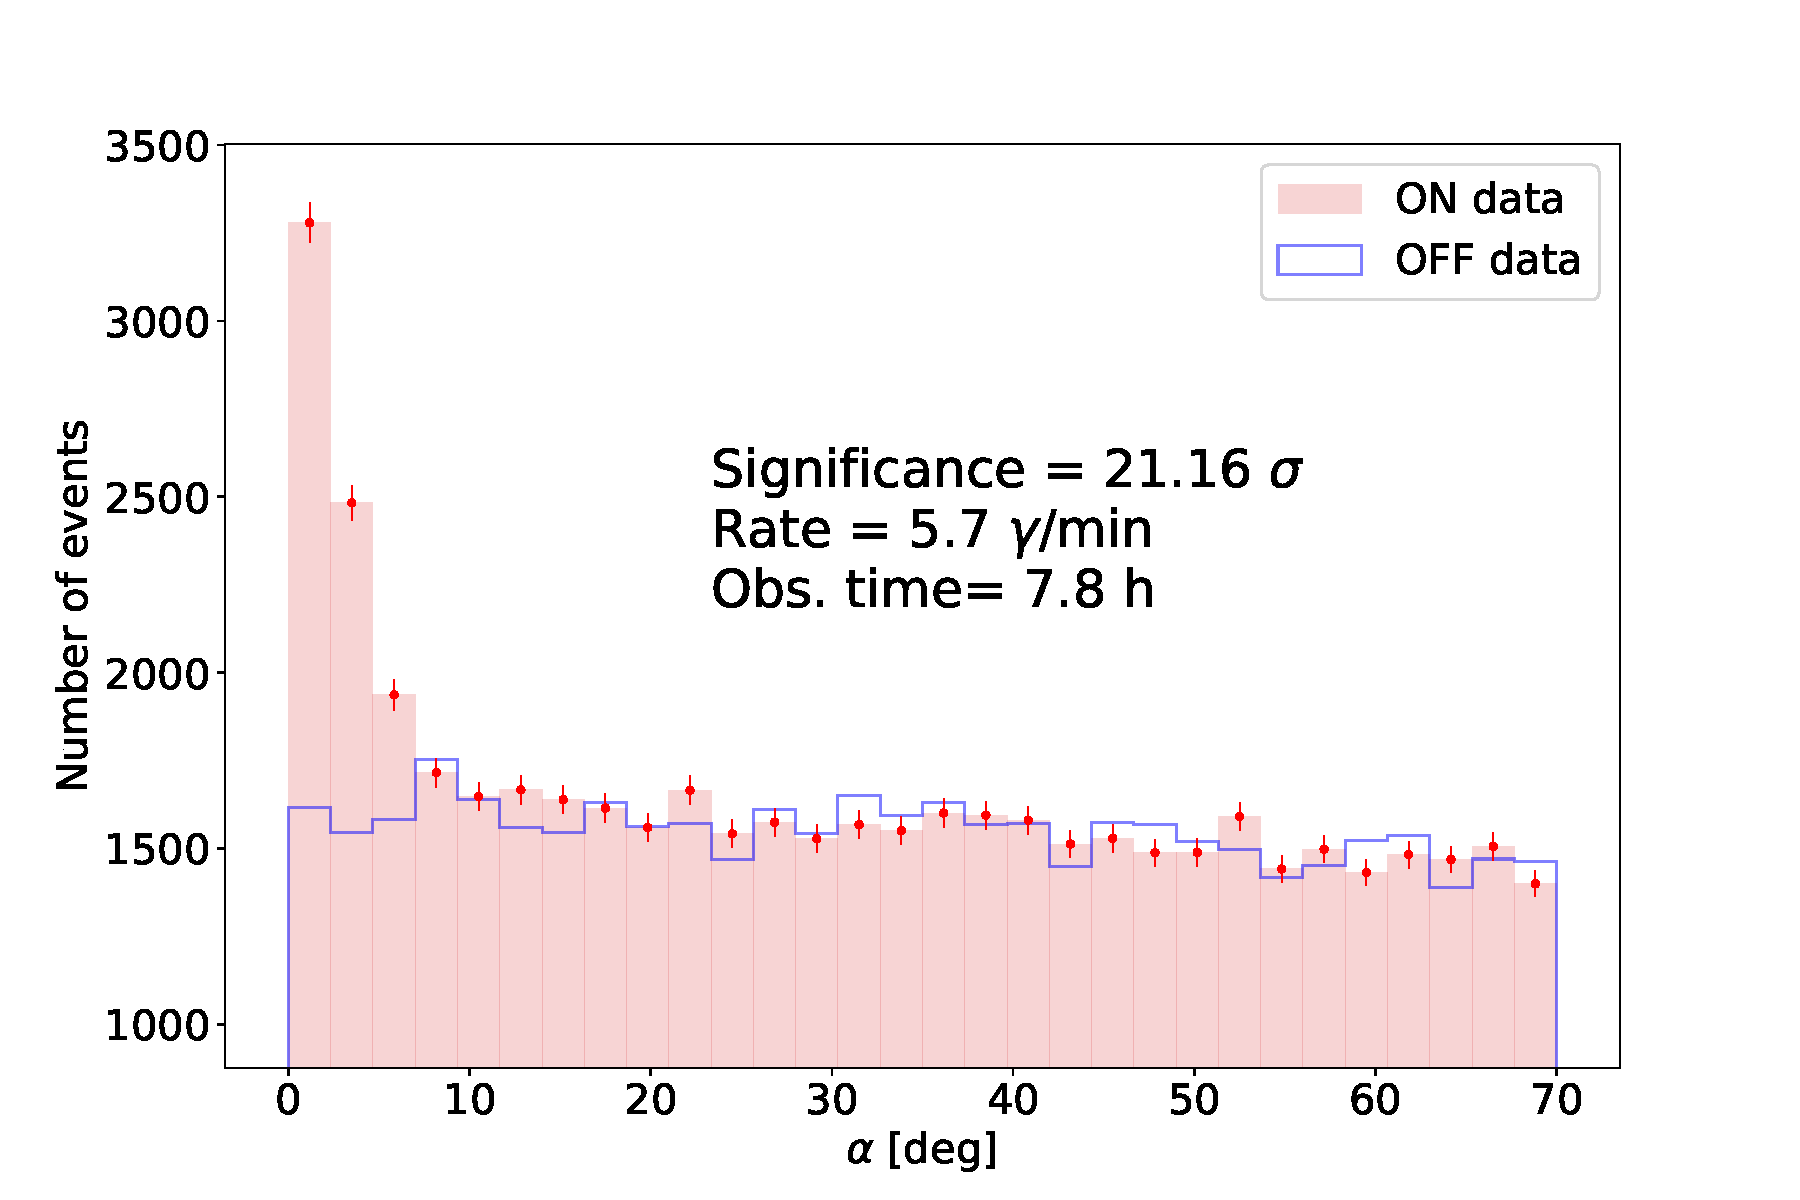
\includegraphics[width=\linewidth]{{Pictures/alphaplot_2ndCrabCampaign_int1000_gammaness0.60}.pdf}
    \caption{\small Intensity > 1000, gammaness > 0.6} \label{fig:2nd-h}
  \end{subfigure}
  \hspace*{\fill} % separation between the subfigures
  \begin{subfigure}{0.32\textwidth}
    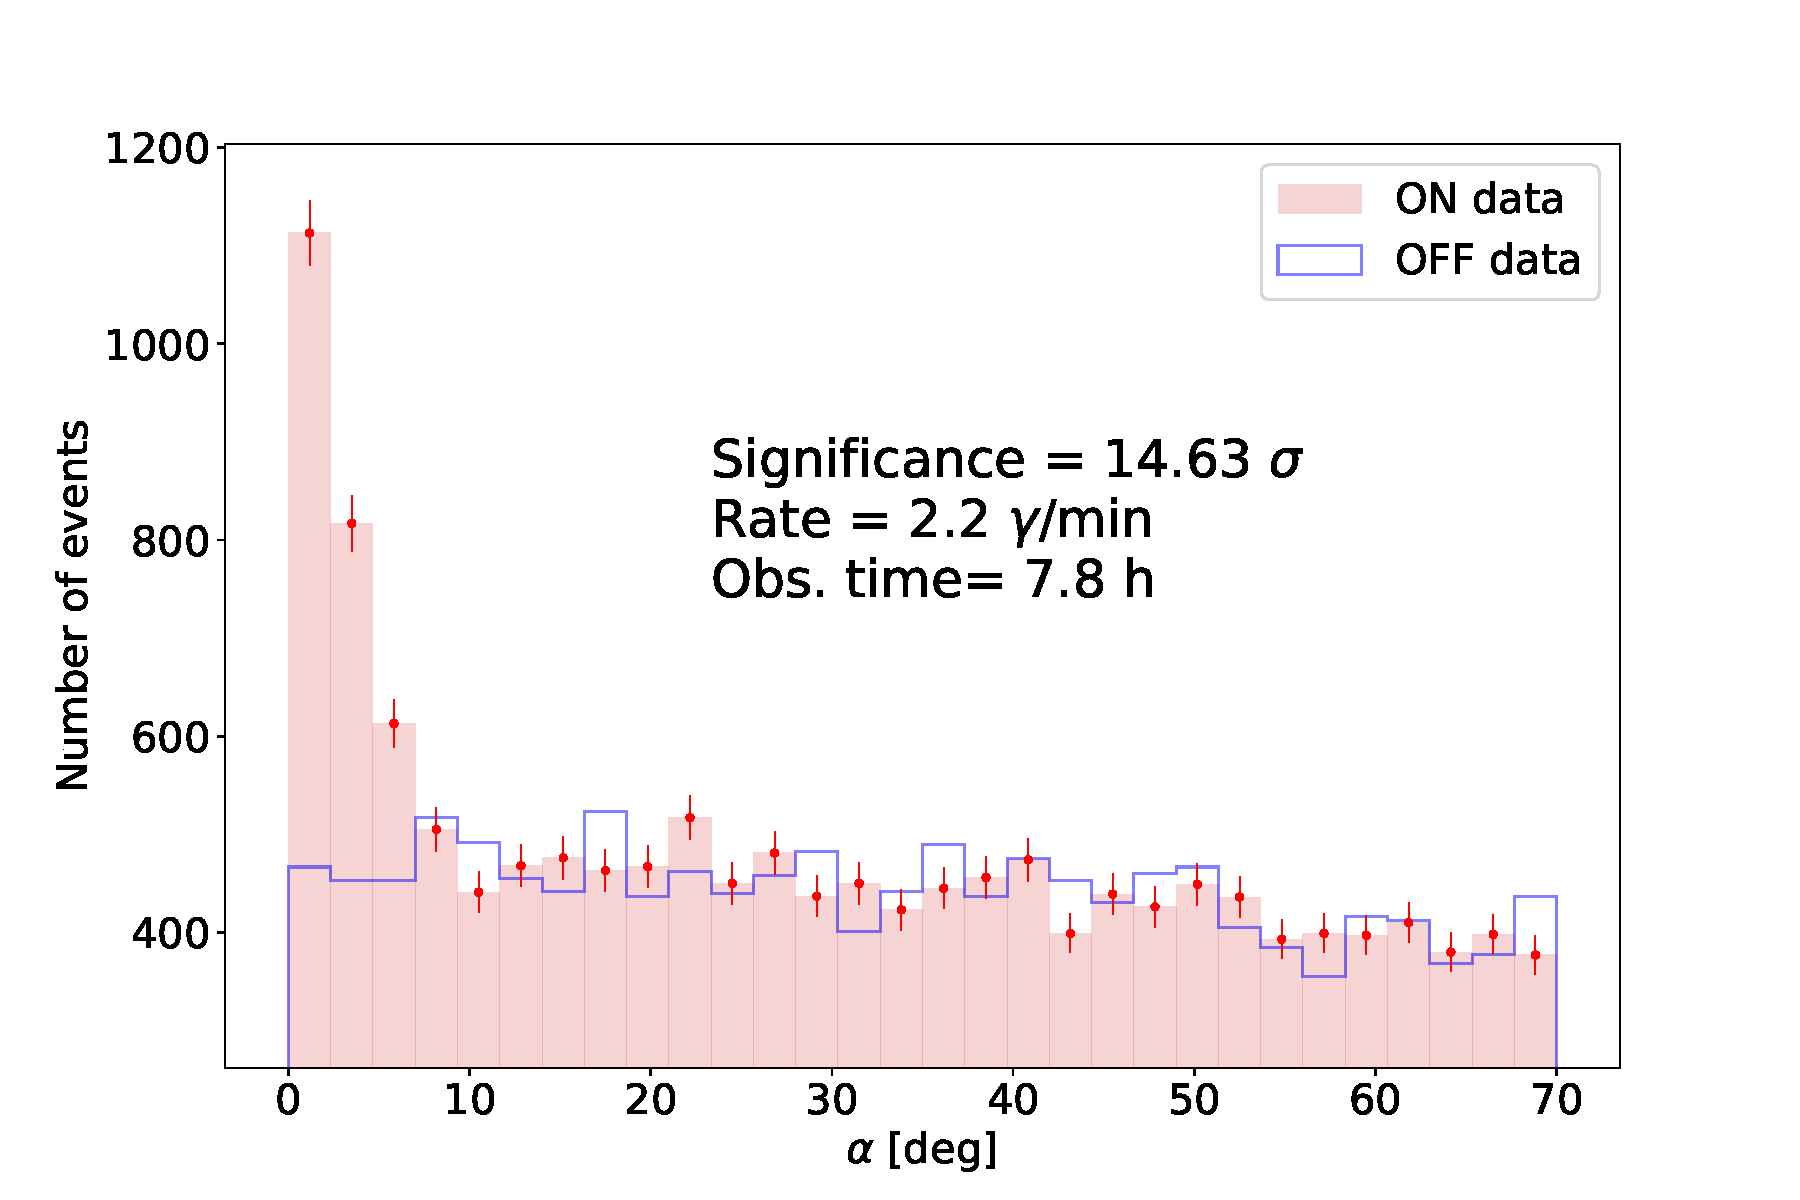
\includegraphics[width=\linewidth]{{Pictures/alphaplot_2ndCrabCampaign_int1000_gammaness0.70}.pdf}
    \caption{\small Intensity > 1000, gammaness > 0.7} \label{fig:2nd-i}
  \end{subfigure}
  \caption{Results of $\alpha$ plot of the Second Crab Campaign of \gls{lst} for different cuts in intensity and gammaness. In each plot the reached significance is shown, defined as explained in section \ref{sec:realdata}, together with the rate of $\gamma$s per minute and the total observation time. \label{fig:2nd-crab-campaign}}
\end{figure}


\begin{figure}[h]
  \begin{subfigure}{0.32\textwidth}
    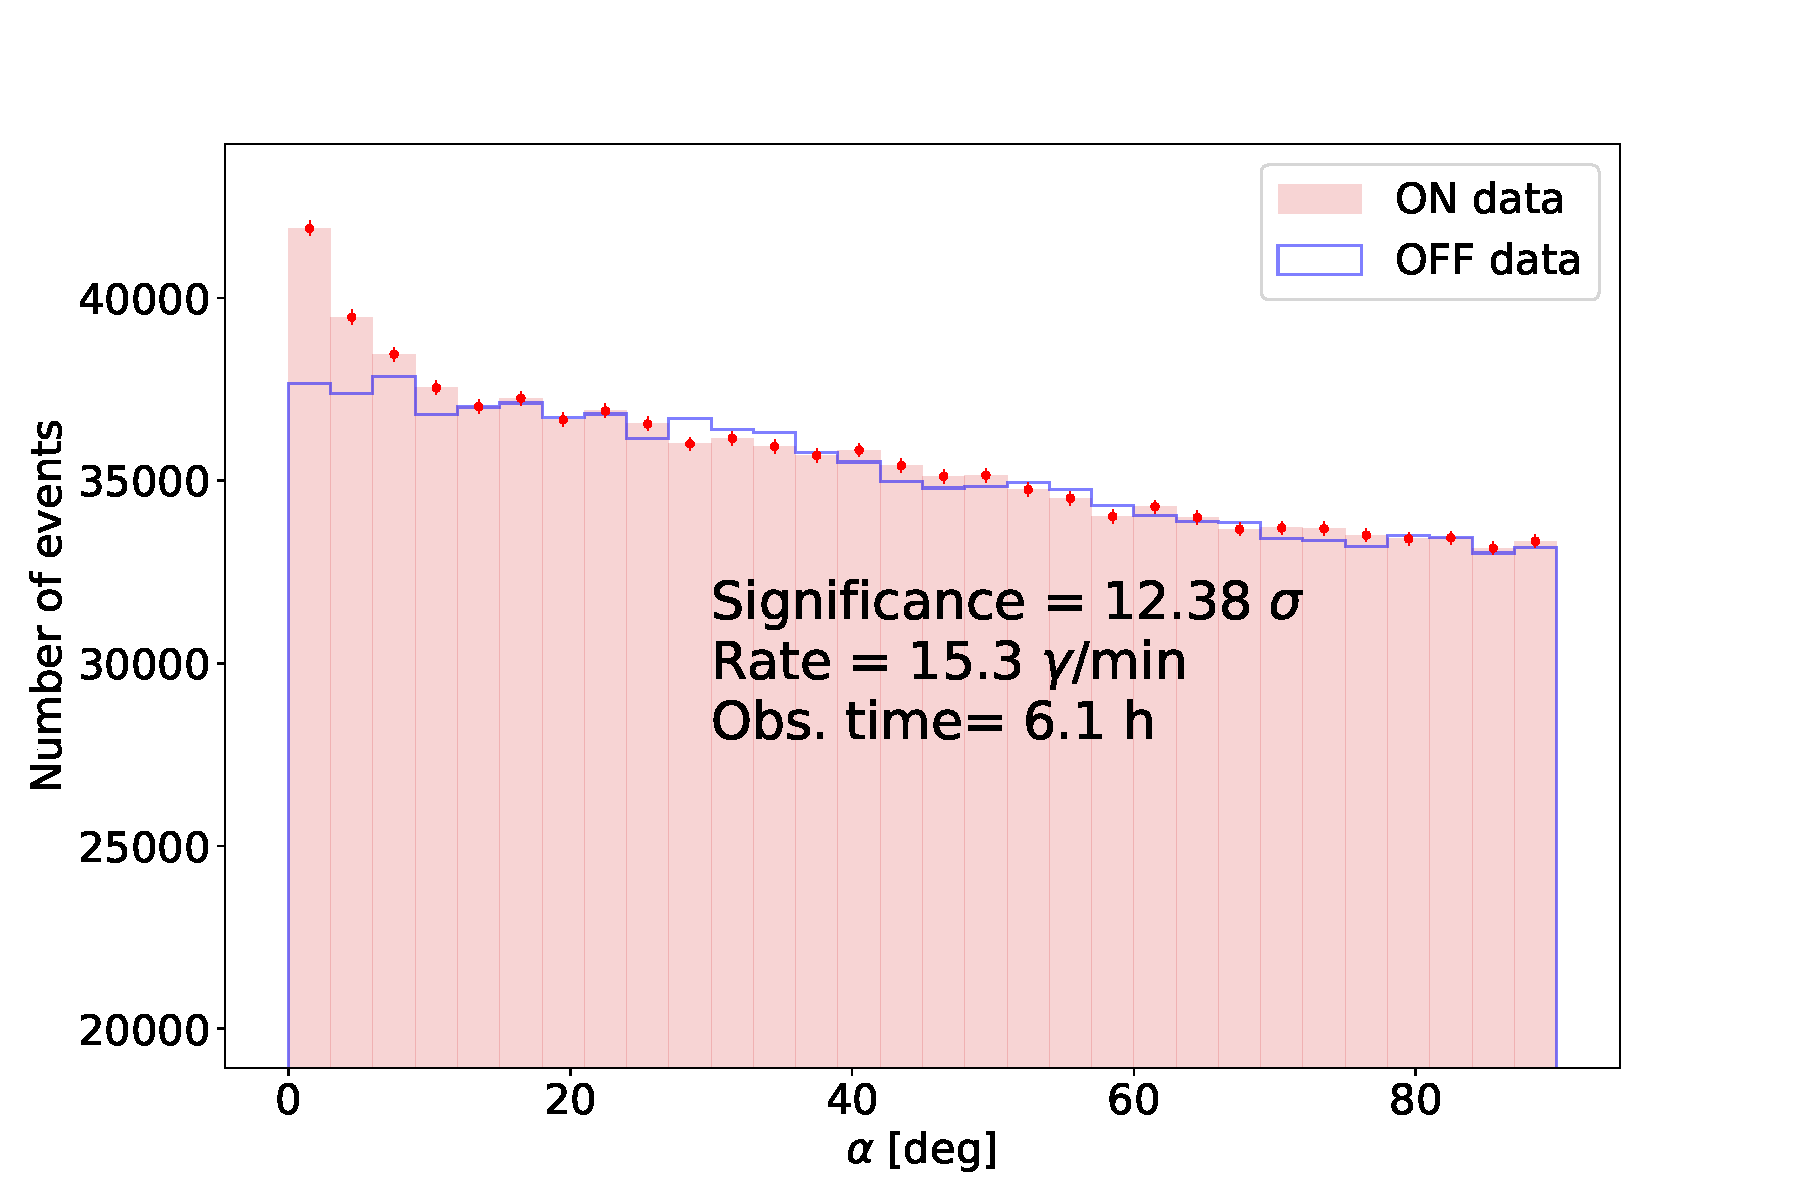
\includegraphics[width=\linewidth]{{Pictures/alphaplot_3rdCrabCampaign_int100_gammaness0.50}.pdf}
    \caption{\small Intensity > 100, gammaness > 0.5} \label{fig:3rd-a}
  \end{subfigure}
  \hspace*{\fill} % separation between the subfigures
  \begin{subfigure}{0.32\textwidth}
    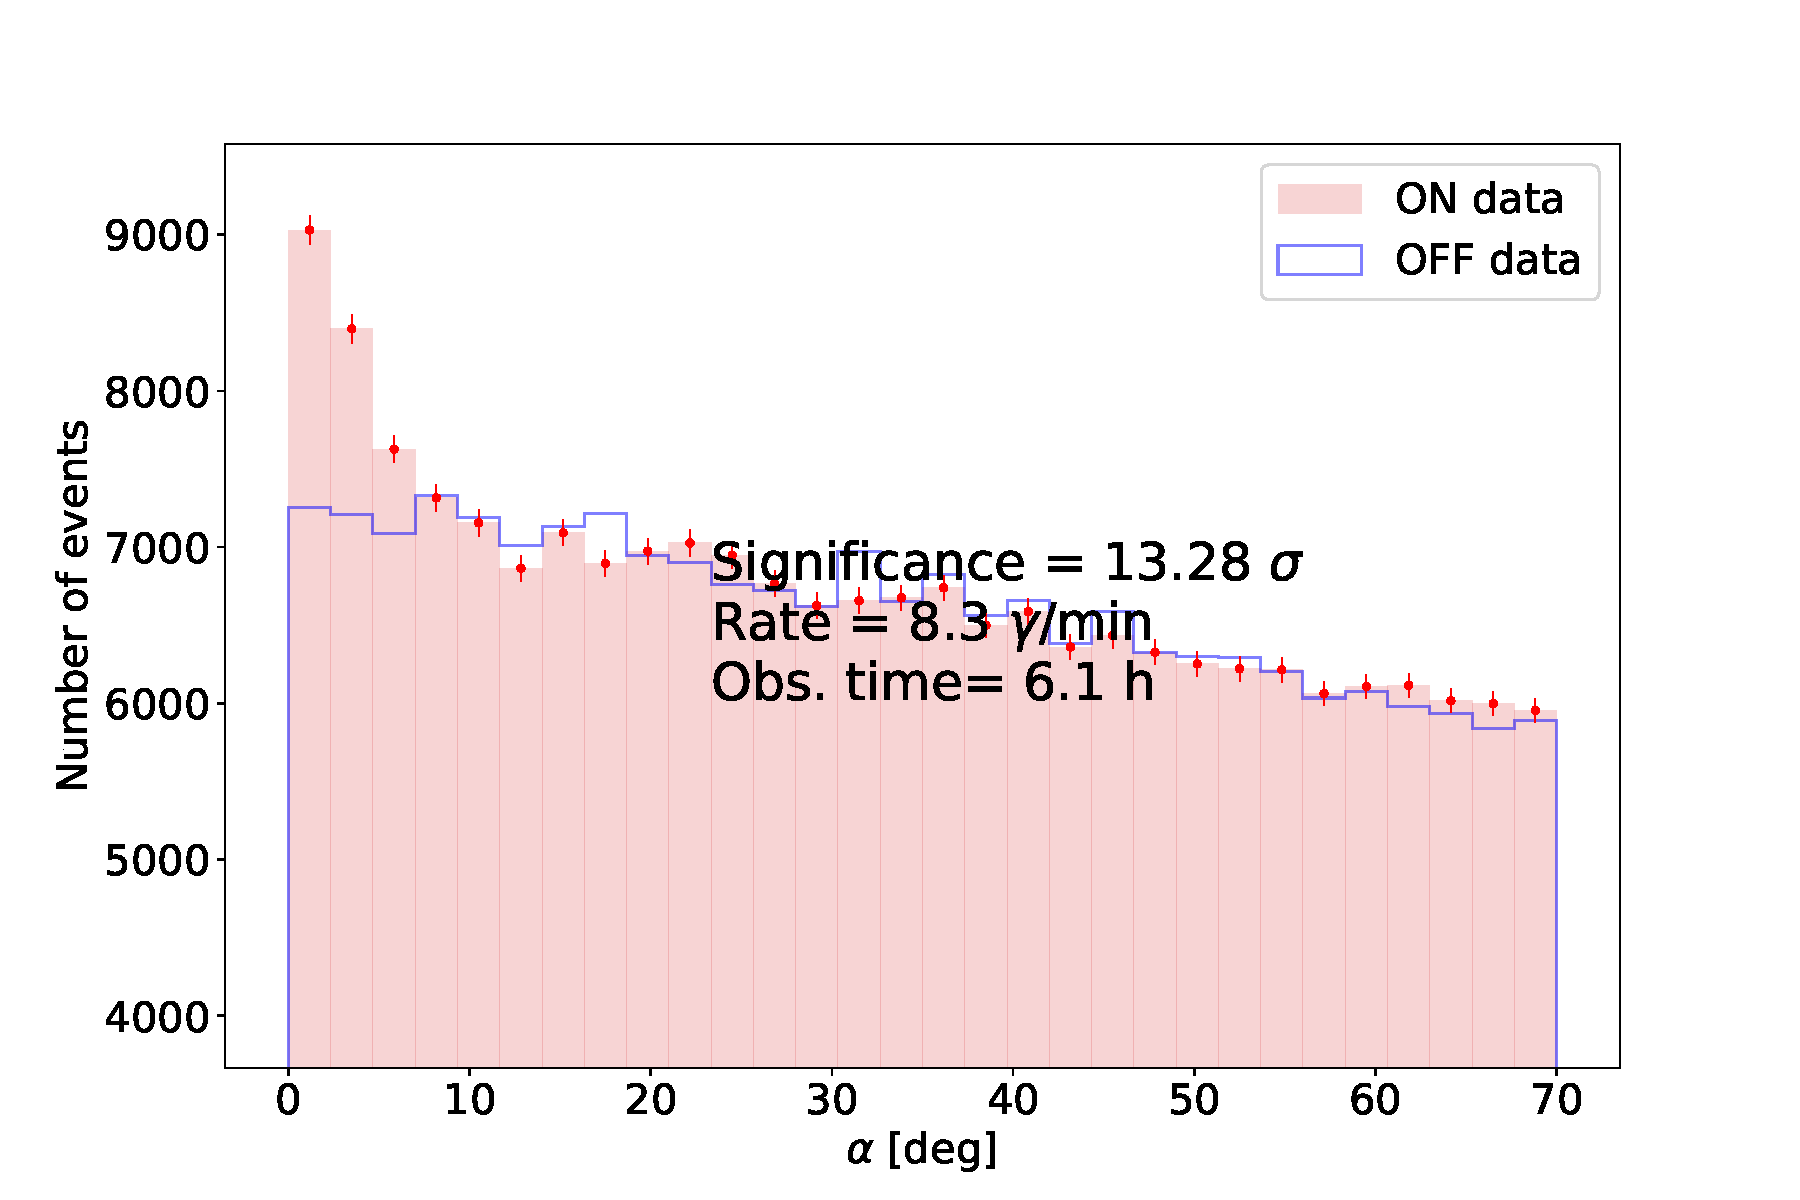
\includegraphics[width=\linewidth]{{Pictures/alphaplot_3rdCrabCampaign_int100_gammaness0.60}.pdf}
    \caption{\small Intensity > 100, gammaness > 0.6} \label{fig:3rd-b}
  \end{subfigure}
  \hspace*{\fill} % separation between the subfigures
  \begin{subfigure}{0.32\textwidth}
    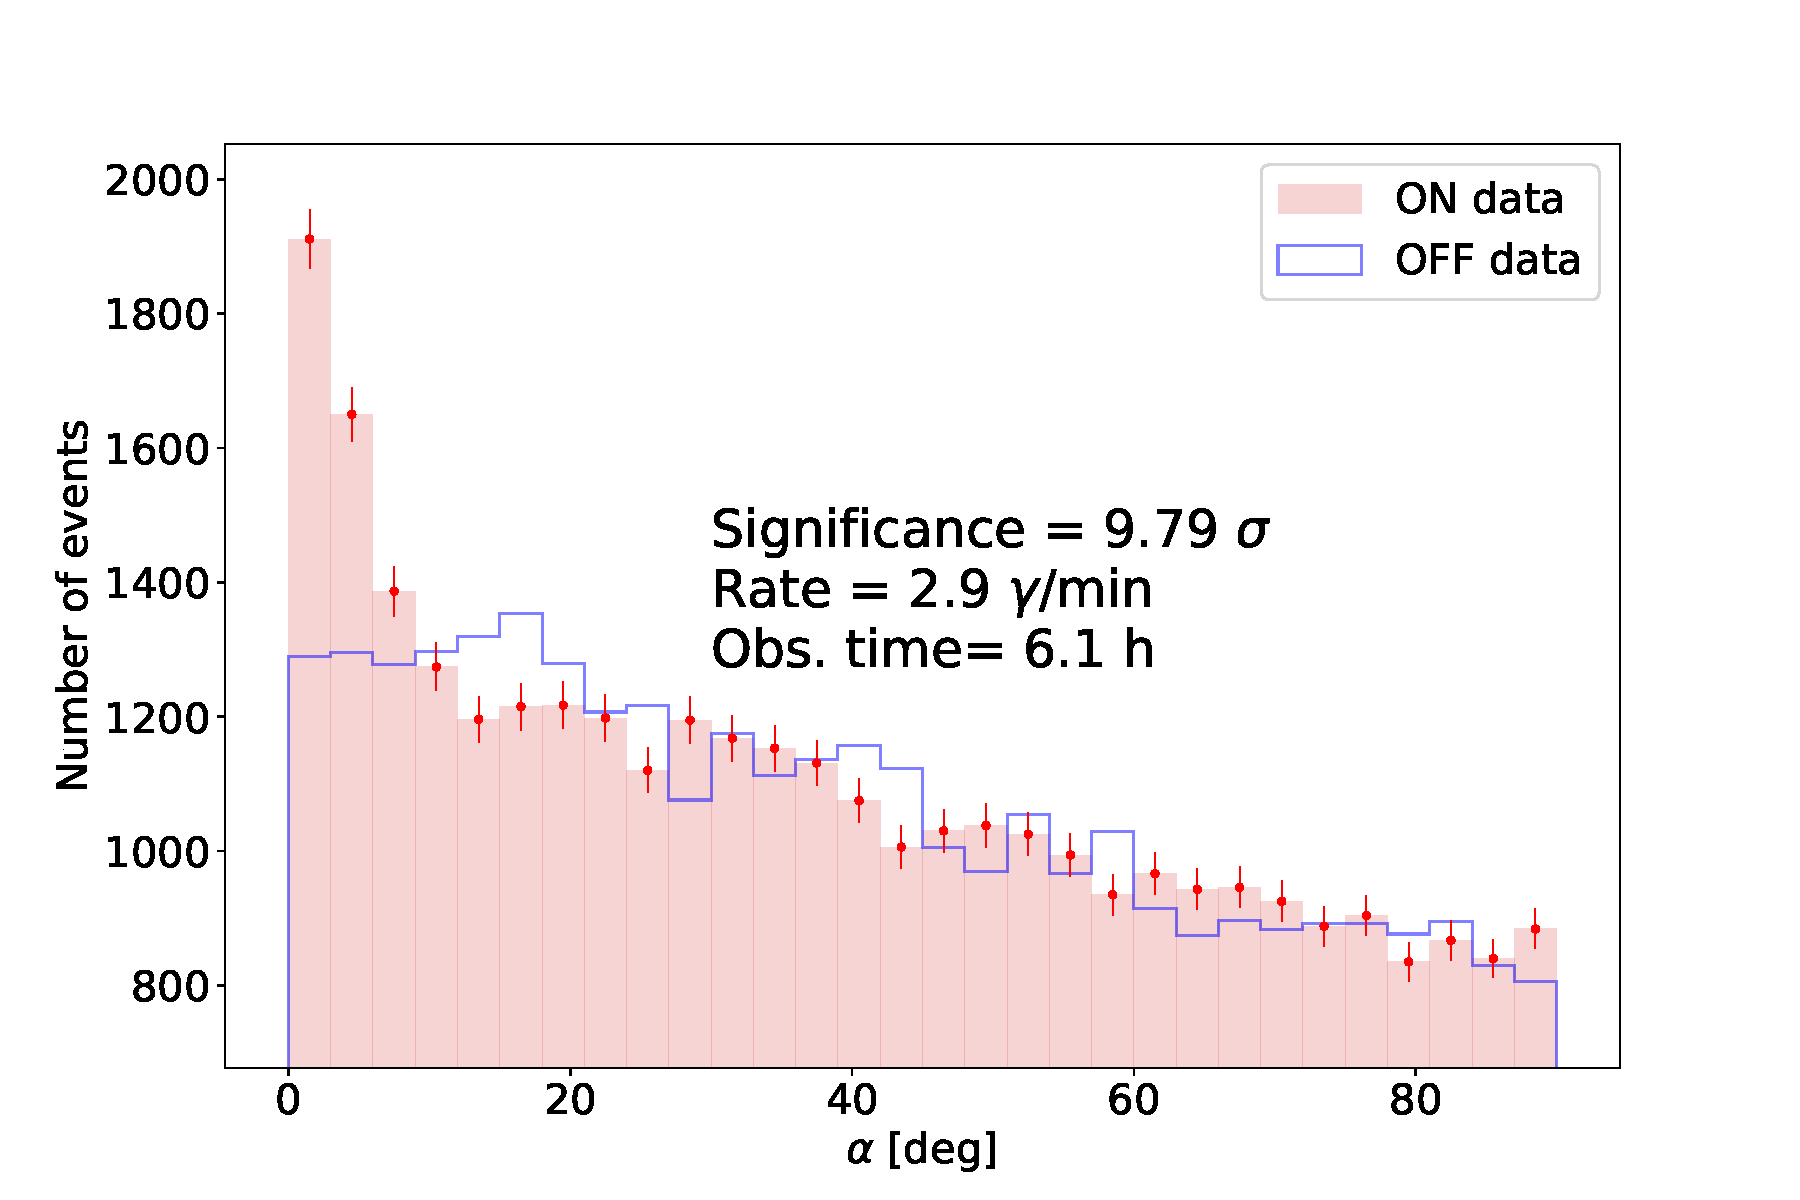
\includegraphics[width=\linewidth]{{Pictures/alphaplot_3rdCrabCampaign_int100_gammaness0.70}.pdf}
    \caption{\small Intensity > 100, gammaness > 0.7} \label{fig:3rd-c}
  \end{subfigure} \\
  \begin{subfigure}{0.32\textwidth}
    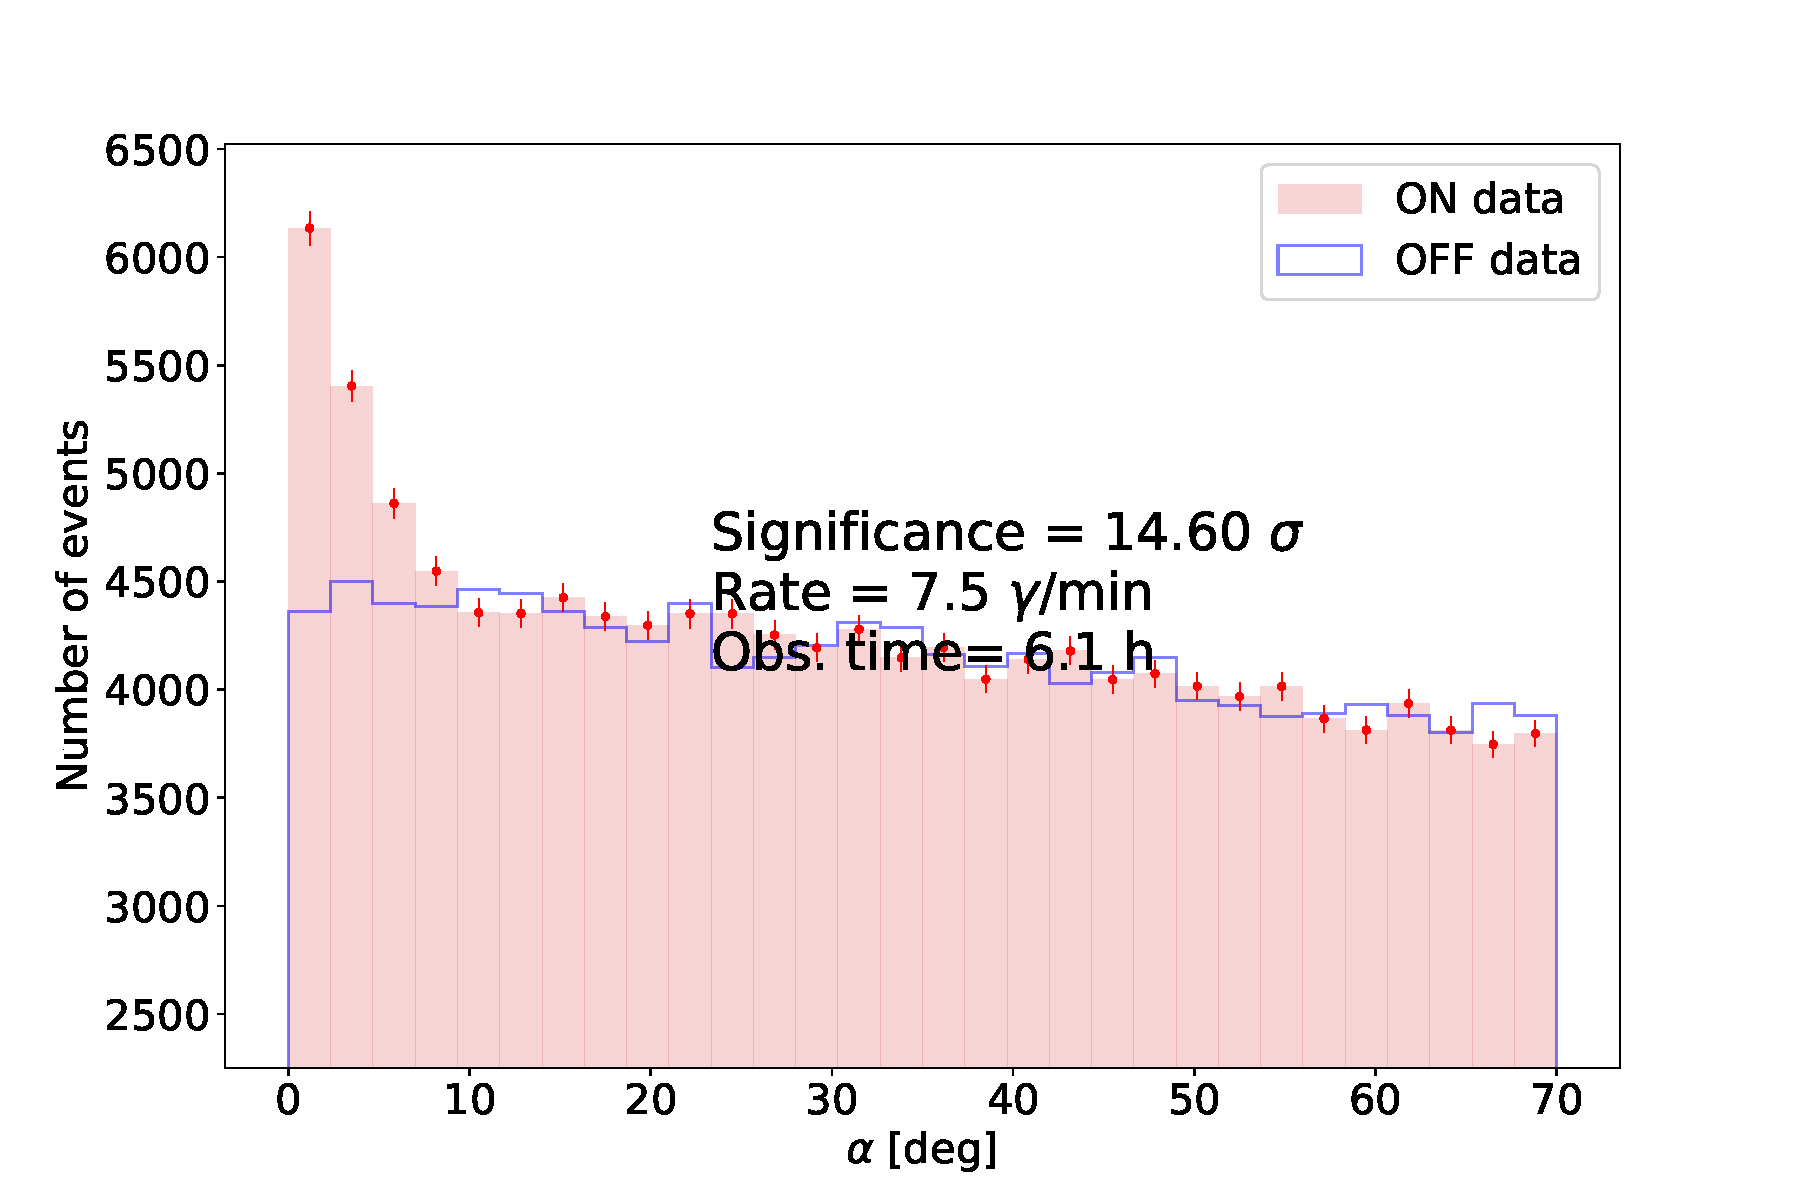
\includegraphics[width=\linewidth]{{Pictures/alphaplot_3rdCrabCampaign_int500_gammaness0.50}.pdf}
    \caption{\small Intensity > 500, gammaness > 0.5} \label{fig:3rd-d}
  \end{subfigure}
  \hspace*{\fill} % separation between the subfigures
  \begin{subfigure}{0.32\textwidth}
    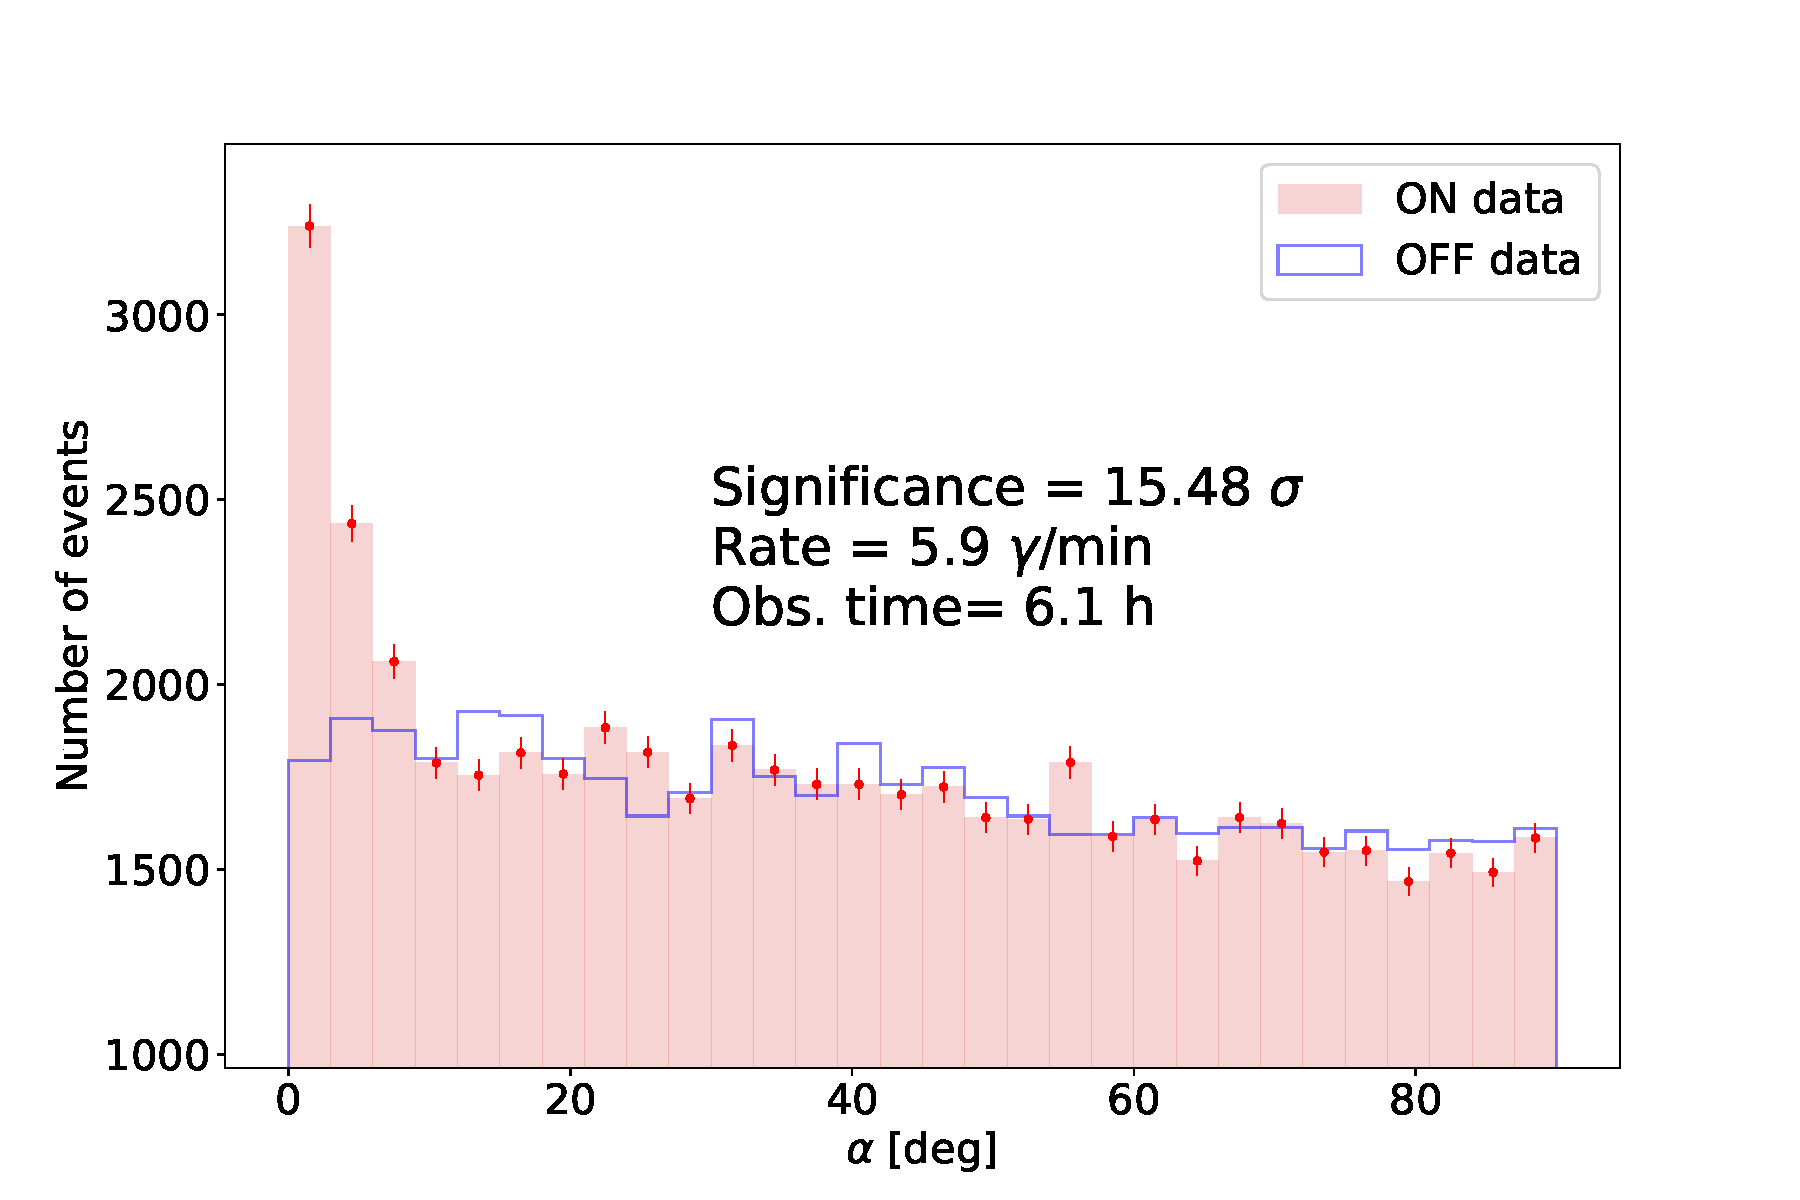
\includegraphics[width=\linewidth]{{Pictures/alphaplot_3rdCrabCampaign_int500_gammaness0.60}.pdf}
    \caption{\small Intensity > 500, gammaness > 0.6} \label{fig:3rd-e}
  \end{subfigure}
  \hspace*{\fill} % separation between the subfigures
  \begin{subfigure}{0.32\textwidth}
    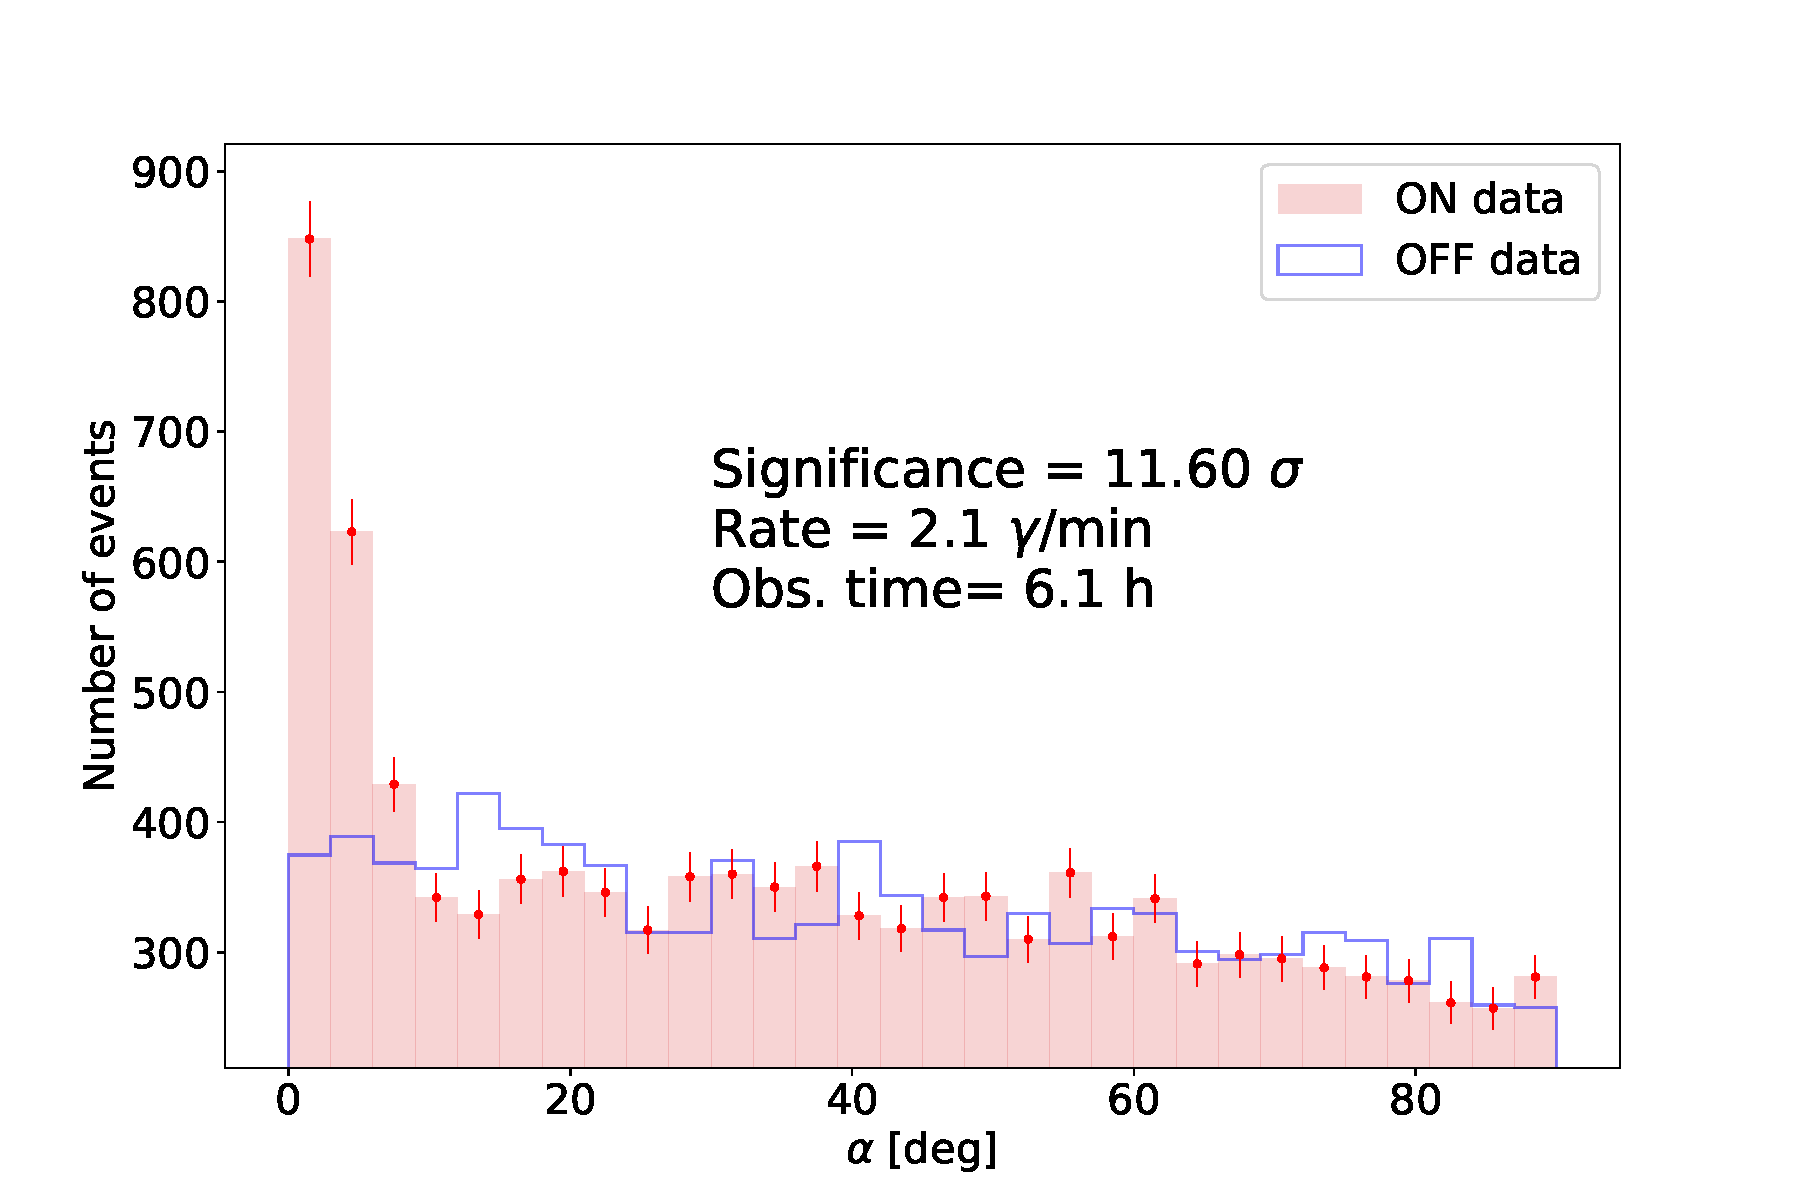
\includegraphics[width=\linewidth]{{Pictures/alphaplot_3rdCrabCampaign_int500_gammaness0.70}.pdf}
    \caption{\small Intensity > 500, gammaness > 0.7} \label{fig:3rd-f}
  \end{subfigure}
  \\
  \begin{subfigure}{0.32\textwidth}
    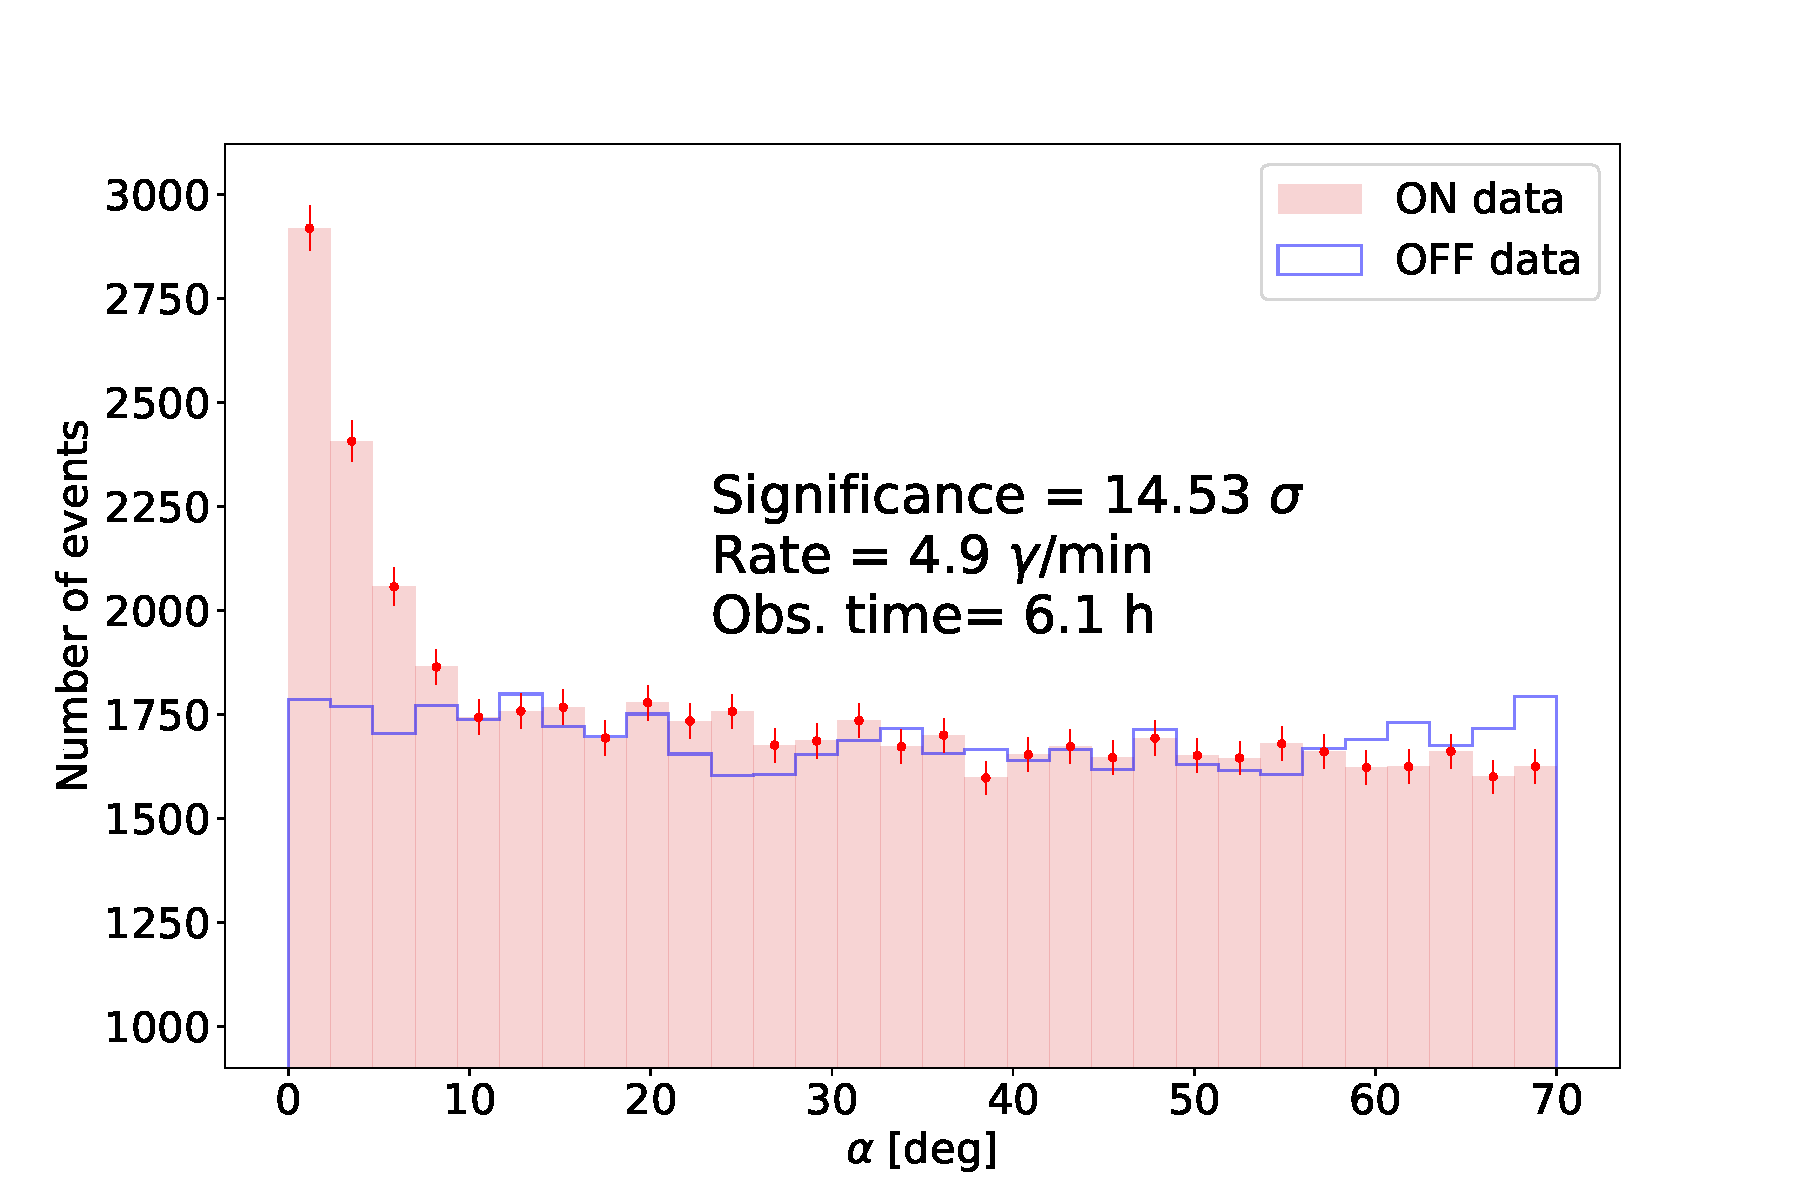
\includegraphics[width=\linewidth]{{Pictures/alphaplot_3rdCrabCampaign_int1000_gammaness0.50}.pdf}
    \caption{\small Intensity > 1000, gammaness > 0.5} \label{fig:3rd-g}
  \end{subfigure}
  \hspace*{\fill} % separation between the subfigures
  \begin{subfigure}{0.32\textwidth}
    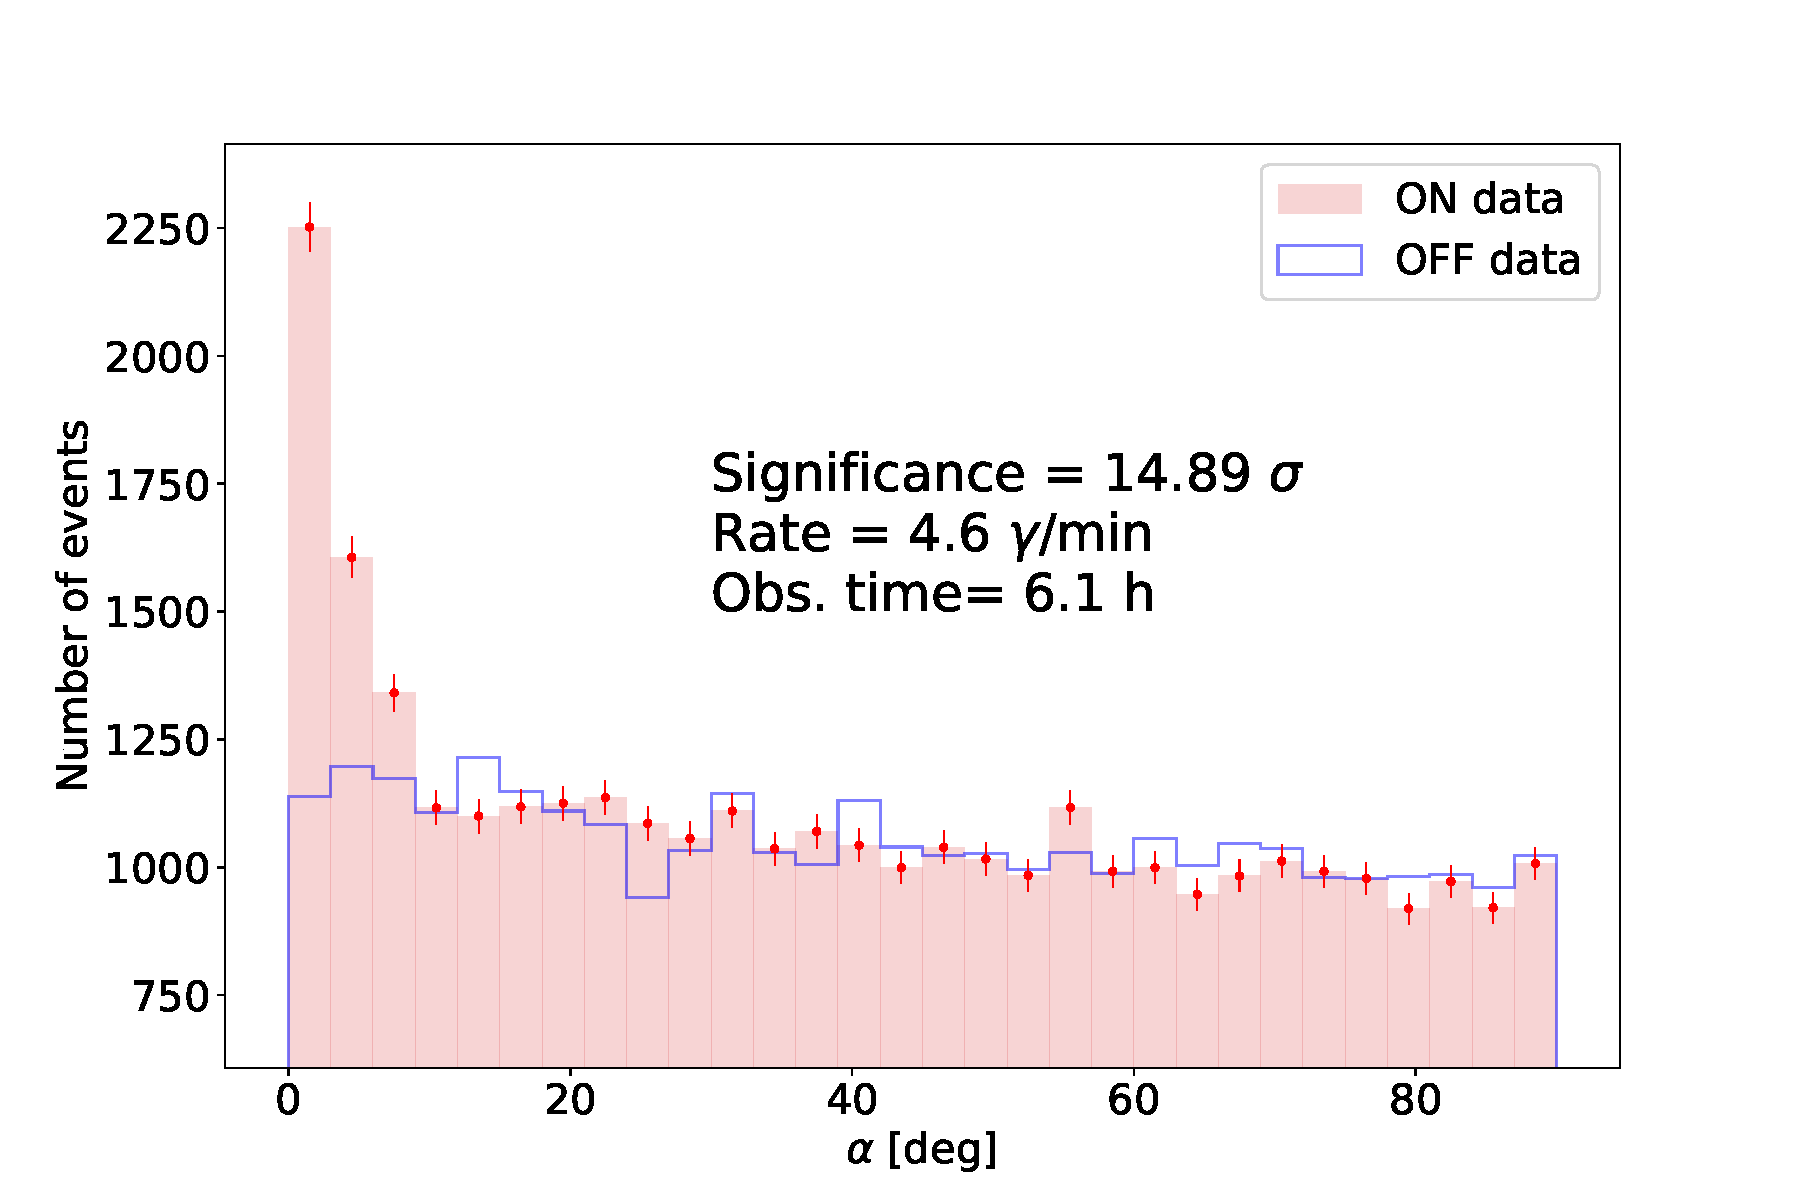
\includegraphics[width=\linewidth]{{Pictures/alphaplot_3rdCrabCampaign_int1000_gammaness0.60}.pdf}
    \caption{\small Intensity > 1000, gammaness > 0.6} \label{fig:3rd-h}
  \end{subfigure}
  \hspace*{\fill} % separation between the subfigures
  \begin{subfigure}{0.32\textwidth}
    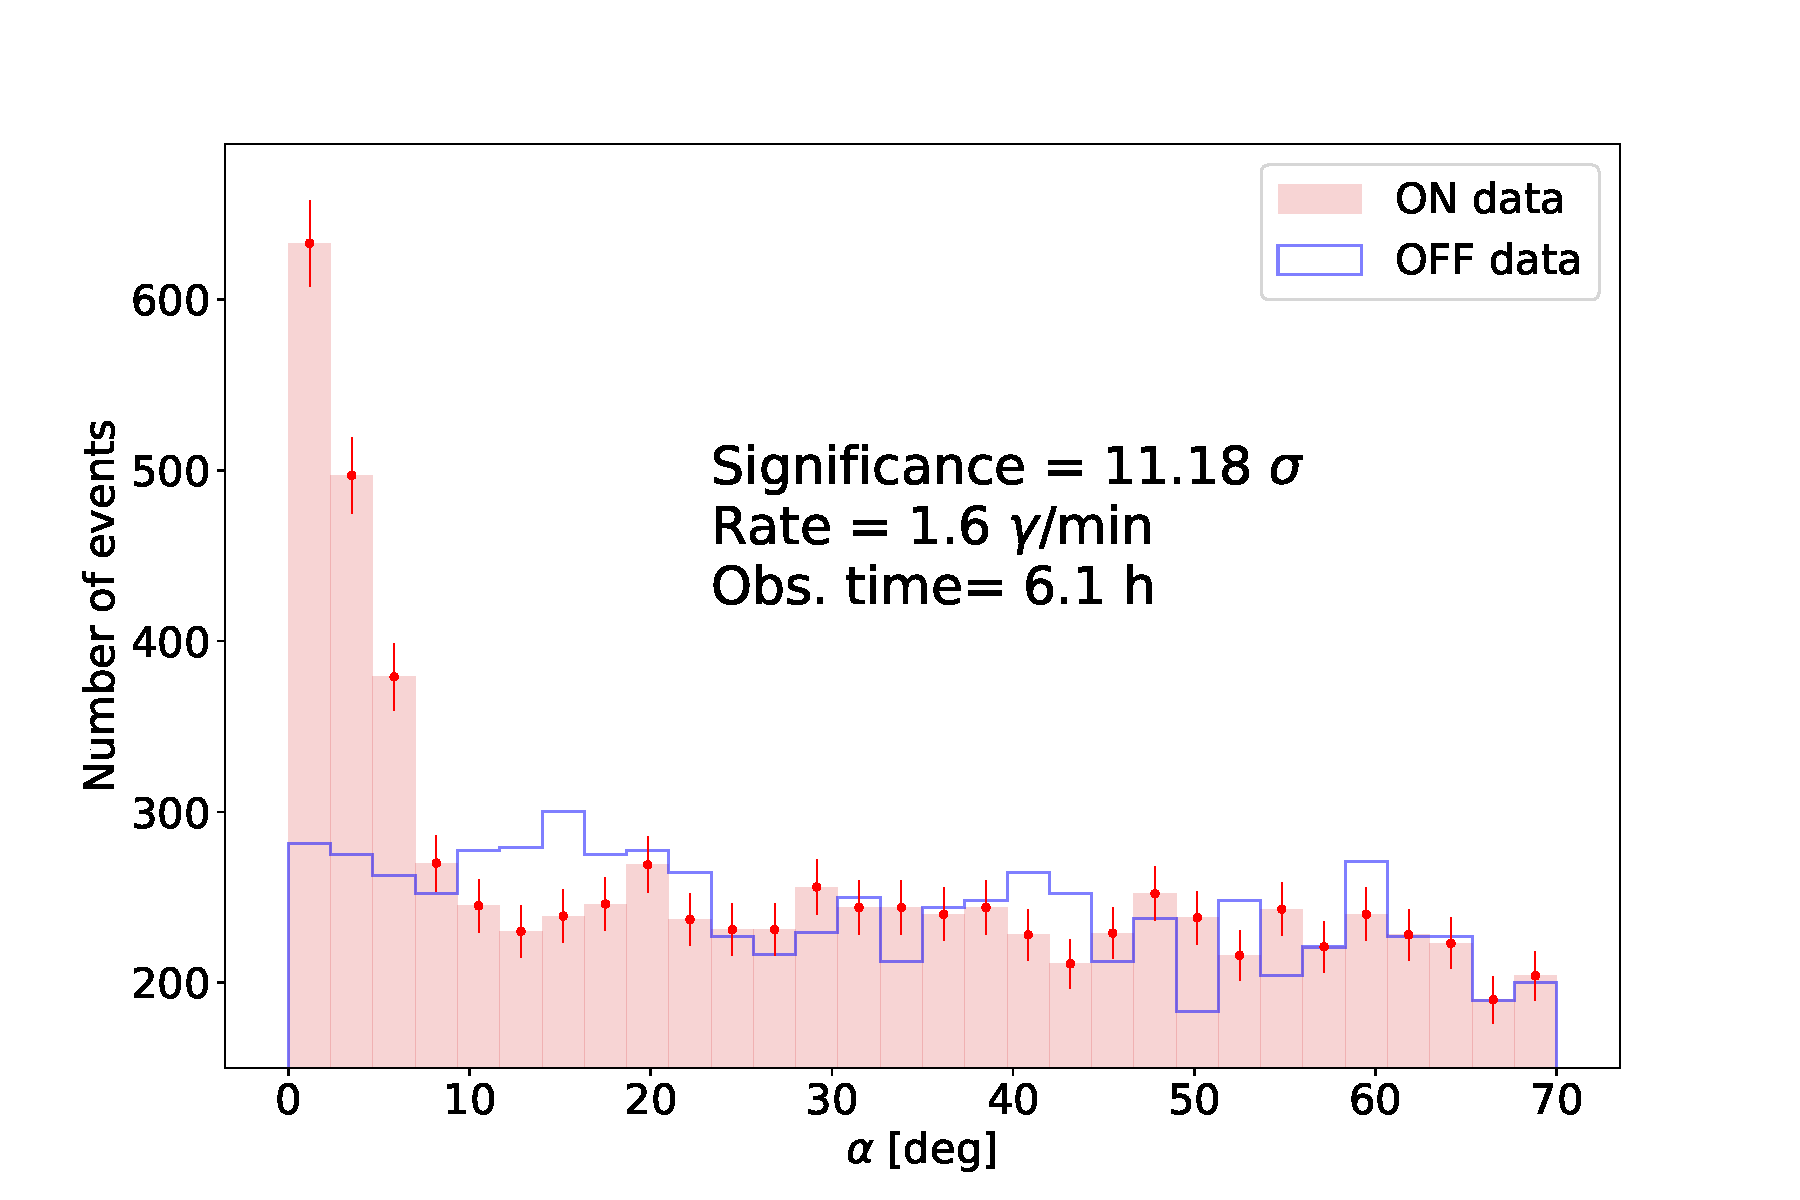
\includegraphics[width=\linewidth]{{Pictures/alphaplot_3rdCrabCampaign_int1000_gammaness0.70}.pdf}
    \caption{\small Intensity > 1000, gammaness > 0.7} \label{fig:3rd-i}
  \end{subfigure}
  \caption{Results of $\alpha$ plot of the Third Crab Campaign of \gls{lst} for different cuts in intensity and gammaness. In each plot the reached significance is shown, defined as explained in section \ref{sec:realdata}, together with the rate of $\gamma$s per minute and the total observation time. \label{fig:3rd-crab-campaign}}
\end{figure}

\outofhere{
  \begin{figure}[h]
    \begin{subfigure}{0.45\textwidth}
      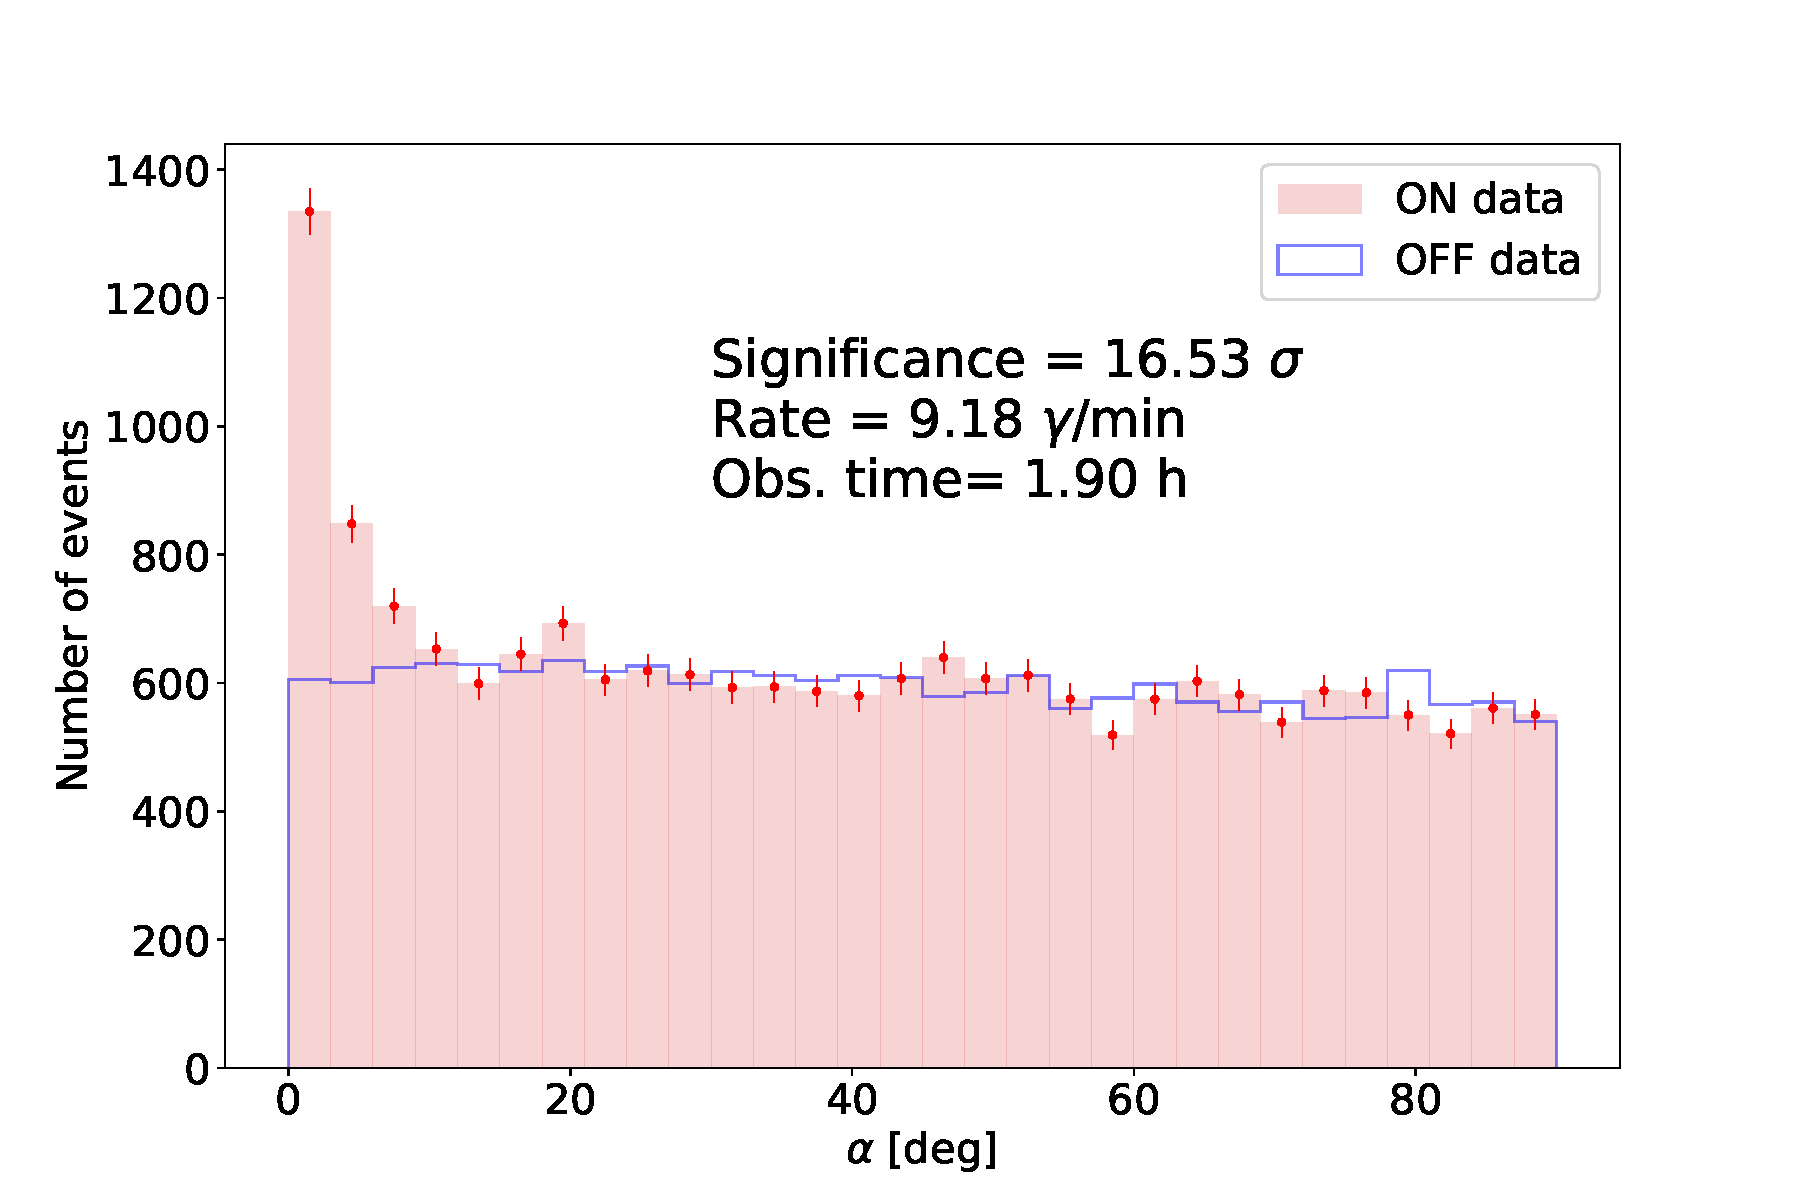
\includegraphics[width=\linewidth]{{Pictures/alphaplot_1stCrabCampaign_20191123_int1000_gammaness0.60}.pdf}
      \caption{\small 23/11/2019} \label{fig:1st-daily-a}
    \end{subfigure}
    \begin{subfigure}{0.45\textwidth}
      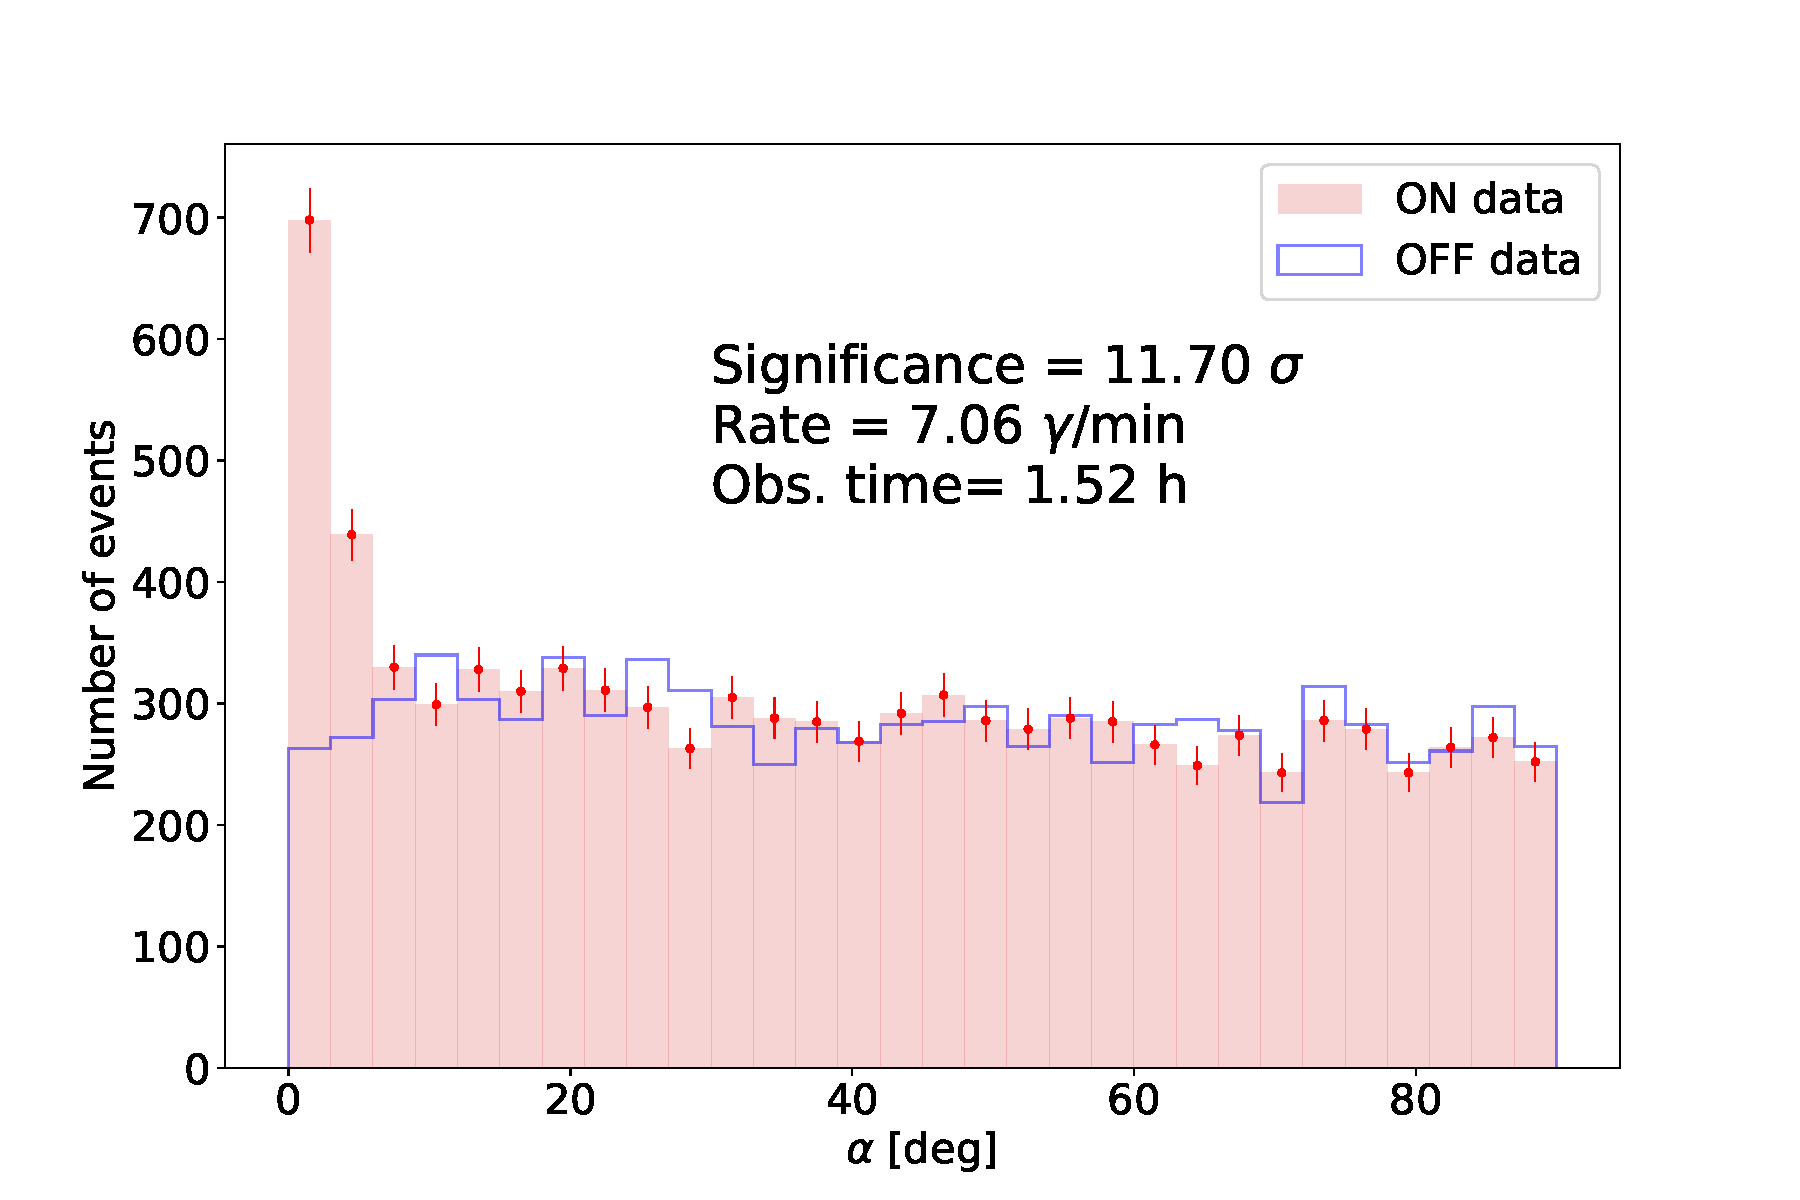
\includegraphics[width=\linewidth]{{Pictures/alphaplot_1stCrabCampaign_20191124_int1000_gammaness0.60}.pdf}
      \caption{\small 24/11/2019} \label{fig:1st-daily-b}
    \end{subfigure} \\
    \begin{subfigure}{0.45\textwidth}
      \includegraphics[width=\linewidth]{{Pictures/alphaplot_1stCrabCampaign_20191126_int1000_gammaness0.60}.pdf}
      \caption{\small 26/11/2019} \label{fig:1st-daily-c}
    \end{subfigure}
    \begin{subfigure}{0.45\textwidth}
      \includegraphics[width=\linewidth]{{Pictures/alphaplot_1stCrabCampaign_20191129_int1000_gammaness0.60}.pdf}
      \caption{\small 29/11/2019} \label{fig:1st-daily-d}
    \end{subfigure}
    \caption{Daily results of $\alpha$ plot of the First Crab Campaign of \gls{lst} for cuts intensity > 1000 and gammaness > 0.6. In each plot the reached significance is shown, defined as explained in section \ref{sec:realdata}, together with the rate of $\gamma$s per minute and the total observation time. \label{fig:1st-crab-campaign-daily}}
  \end{figure}

  \begin{figure}[h]
    \begin{subfigure}{0.45\textwidth}
      \includegraphics[width=\linewidth]{{Pictures/alphaplot_2ndCrabCampaign_20200115_int1000_gammaness0.60}.pdf}
      \caption{\small 15/01/2020} \label{fig:2nd-daily-a}
    \end{subfigure}
    \begin{subfigure}{0.45\textwidth}
      \includegraphics[width=\linewidth]{{Pictures/alphaplot_2ndCrabCampaign_20200117_int1000_gammaness0.60}.pdf}
      \caption{\small 17/01/2020} \label{fig:2nd-daily-b}
    \end{subfigure} \\
    \begin{subfigure}{0.45\textwidth}
      \includegraphics[width=\linewidth]{{Pictures/alphaplot_2ndCrabCampaign_20200118_int500_gammaness0.60}.pdf}
      \caption{\small 18/01/2020} \label{fig:2nd-daily-c}
    \end{subfigure}
    \begin{subfigure}{0.45\textwidth}
      \includegraphics[width=\linewidth]{{Pictures/alphaplot_2ndCrabCampaign_20200127_int500_gammaness0.60}.pdf}
      \caption{\small 27/01/2020} \label{fig:2nd-daily-d}
    \end{subfigure} \\
    \begin{subfigure}{0.45\textwidth}
      \includegraphics[width=\linewidth]{{Pictures/alphaplot_2ndCrabCampaign_20200128_int500_gammaness0.60}.pdf}
      \caption{\small 28/01/2020} \label{fig:2nd-daily-c}
    \end{subfigure}
    \caption{Daily results of $\alpha$ plot of the Second Crab Campaign of \gls{lst} for cuts intensity > 500 and gammaness > 0.6, except for days 15/01/2020 and 17/01/2020 where a cut in intensity > 1000 resulted in a better significance. In each plot the reached significance is shown, defined as explained in section \ref{sec:realdata}, together with the rate of $\gamma$s per minute and the total observation time. \label{fig:2nd-crab-campaign-daily}}
  \end{figure}


  \begin{figure}[h]
    \begin{subfigure}{0.45\textwidth}
      \includegraphics[width=\linewidth]{{Pictures/alphaplot_3rdCrabCampaign_20200213_int500_gammaness0.60}.pdf}
      \caption{\small 13/02/2020} \label{fig:3rd-daily-a}
    \end{subfigure}
    \begin{subfigure}{0.45\textwidth}
      \includegraphics[width=\linewidth]{{Pictures/alphaplot_3rdCrabCampaign_20200215_int500_gammaness0.60}.pdf}
      \caption{\small 15/02/2020} \label{fig:3rd-daily-b}
    \end{subfigure} \\
    \begin{subfigure}{0.45\textwidth}
      \includegraphics[width=\linewidth]{{Pictures/alphaplot_3rdCrabCampaign_20200217_int500_gammaness0.60}.pdf}
      \caption{\small 17/02/2020} \label{fig:3rd-daily-c}
    \end{subfigure}
    \begin{subfigure}{0.45\textwidth}
      \includegraphics[width=\linewidth]{{Pictures/alphaplot_3rdCrabCampaign_20200218_int1000_gammaness0.60}.pdf}
      \caption{\small 18/02/2020} \label{fig:3rd-daily-d}
    \end{subfigure} \\
    \begin{subfigure}{0.45\textwidth}
      \includegraphics[width=\linewidth]{{Pictures/alphaplot_3rdCrabCampaign_20200228_int500_gammaness0.60}.pdf}
      \caption{\small 28/02/2020} \label{fig:3rd-daily-d}
    \end{subfigure}\\
    \caption{Daily results of $\alpha$ plot of the Third Crab Campaign of \gls{lst} for cuts intensity > 500 and gammaness > 0.6, except for 18/02/2020 where a cut in intensity > 1000 resulted in a better significance. In each plot the reached significance is shown, defined as explained in section \ref{sec:realdata}, together with the rate of $\gamma$s per minute and the total observation time. \label{fig:3rd-crab-campaign-daily}}
  \end{figure}
}

\begin{figure}[t]
  \begin{subfigure}{0.32\textwidth}
    \includegraphics[width=\linewidth]{{Pictures/em_alphaplot_1stCrabCampaign_int100_gammaness0.60}.pdf}
    \caption{\small Intensity > 100, gammaness > 0.6} \label{fig:em_1st-a}
  \end{subfigure}
  \hspace*{\fill} % separation between the subfigures
  \begin{subfigure}{0.32\textwidth}
    \includegraphics[width=\linewidth]{{Pictures/em_alphaplot_1stCrabCampaign_int100_gammaness0.70}.pdf}
    \caption{\small Intensity > 100, gammaness > 0.7} \label{fig:em_1st-b}
  \end{subfigure}
  \hspace*{\fill} % separation between the subfigures
  \begin{subfigure}{0.32\textwidth}
    \includegraphics[width=\linewidth]{{Pictures/em_alphaplot_1stCrabCampaign_int100_gammaness0.80}.pdf}
    \caption{\small Intensity > 100, gammaness > 0.8} \label{fig:em_1st-c}
  \end{subfigure} \\
  \begin{subfigure}{0.32\textwidth}
    \includegraphics[width=\linewidth]{{Pictures/em_alphaplot_1stCrabCampaign_int500_gammaness0.60}.pdf}
    \caption{\small Intensity > 500, gammaness > 0.6} \label{fig:em_1st-d}
  \end{subfigure}
  \hspace*{\fill} % separation between the subfigures
  \begin{subfigure}{0.32\textwidth}
    \includegraphics[width=\linewidth]{{Pictures/em_alphaplot_1stCrabCampaign_int500_gammaness0.70}.pdf}
    \caption{\small Intensity > 500, gammaness > 0.7} \label{fig:em_1st-e}
  \end{subfigure}
  \hspace*{\fill} % separation between the subfigures
  \begin{subfigure}{0.32\textwidth}
    \includegraphics[width=\linewidth]{{Pictures/em_alphaplot_1stCrabCampaign_int500_gammaness0.80}.pdf}
    \caption{\small Intensity > 500, gammaness > 0.8} \label{fig:em_1st-f}
  \end{subfigure}
  \\
  \begin{subfigure}{0.32\textwidth}
    \includegraphics[width=\linewidth]{{Pictures/em_alphaplot_1stCrabCampaign_int1000_gammaness0.60}.pdf}
    \caption{\small Intensity > 1000, gammaness > 0.6} \label{fig:em_1st-g}
  \end{subfigure}
  \hspace*{\fill} % separation between the subfigures
  \begin{subfigure}{0.32\textwidth}
    \includegraphics[width=\linewidth]{{Pictures/em_alphaplot_1stCrabCampaign_int1000_gammaness0.70}.pdf}
    \caption{\small Intensity > 1000, gammaness > 0.7} \label{fig:em_1st-h}
  \end{subfigure}
  \hspace*{\fill} % separation between the subfigures
  \begin{subfigure}{0.32\textwidth}
    \includegraphics[width=\linewidth]{{Pictures/em_alphaplot_1stCrabCampaign_int1000_gammaness0.80}.pdf}
    \caption{\small Intensity > 1000, gammaness > 0.8} \label{fig:em_1st-i}
  \end{subfigure}
  \caption{Results of $\alpha$ plot of the First Crab Campaign of \gls{lst}, analyzed using the \gls{em} method for Hillas parameterization, for different cuts in intensity and gammaness. In each plot the reached significance is shown, defined as explained in section \ref{sec:realdata}, together with the rate of $\gamma$s per minute and the total observation time. \label{fig:em_1st-crab-campaign}}
\end{figure}

\begin{figure}[t]
  \begin{subfigure}{0.32\textwidth}
    \includegraphics[width=\linewidth]{{Pictures/em_alphaplot_2ndCrabCampaign_int100_gammaness0.60}.pdf}
    \caption{\small Intensity > 100, gammaness > 0.6} \label{fig:em_2nd-a}
  \end{subfigure}
  \hspace*{\fill} % separation between the subfigures
  \begin{subfigure}{0.32\textwidth}
    \includegraphics[width=\linewidth]{{Pictures/em_alphaplot_2ndCrabCampaign_int100_gammaness0.70}.pdf}
    \caption{\small Intensity > 100, gammaness > 0.7} \label{fig:em_2nd-b}
  \end{subfigure}
  \hspace*{\fill} % separation between the subfigures
  \begin{subfigure}{0.32\textwidth}
    \includegraphics[width=\linewidth]{{Pictures/em_alphaplot_2ndCrabCampaign_int100_gammaness0.80}.pdf}
    \caption{\small Intensity > 100, gammaness > 0.8} \label{fig:em_2nd-c}
  \end{subfigure} \\
  \begin{subfigure}{0.32\textwidth}
    \includegraphics[width=\linewidth]{{Pictures/em_alphaplot_2ndCrabCampaign_int500_gammaness0.60}.pdf}
    \caption{\small Intensity > 500, gammaness > 0.6} \label{fig:em_2nd-d}
  \end{subfigure}
  \hspace*{\fill} % separation between the subfigures
  \begin{subfigure}{0.32\textwidth}
    \includegraphics[width=\linewidth]{{Pictures/em_alphaplot_2ndCrabCampaign_int500_gammaness0.70}.pdf}
    \caption{\small Intensity > 500, gammaness > 0.7} \label{fig:em_2nd-e}
  \end{subfigure}
  \hspace*{\fill} % separation between the subfigures
  \begin{subfigure}{0.32\textwidth}
    \includegraphics[width=\linewidth]{{Pictures/em_alphaplot_2ndCrabCampaign_int500_gammaness0.80}.pdf}
    \caption{\small Intensity > 500, gammaness > 0.8} \label{fig:em_2nd-f}
  \end{subfigure}
  \\
  \begin{subfigure}{0.32\textwidth}
    \includegraphics[width=\linewidth]{{Pictures/em_alphaplot_2ndCrabCampaign_int1000_gammaness0.60}.pdf}
    \caption{\small Intensity > 1000, gammaness > 0.6} \label{fig:em_2nd-g}
  \end{subfigure}
  \hspace*{\fill} % separation between the subfigures
  \begin{subfigure}{0.32\textwidth}
    \includegraphics[width=\linewidth]{{Pictures/em_alphaplot_2ndCrabCampaign_int1000_gammaness0.70}.pdf}
    \caption{\small Intensity > 1000, gammaness > 0.7} \label{fig:em_2nd-h}
  \end{subfigure}
  \hspace*{\fill} % separation between the subfigures
  \begin{subfigure}{0.32\textwidth}
    \includegraphics[width=\linewidth]{{Pictures/em_alphaplot_2ndCrabCampaign_int1000_gammaness0.80}.pdf}
    \caption{\small Intensity > 1000, gammaness > 0.8} \label{fig:em_2nd-i}
  \end{subfigure}
  \caption{Results of $\alpha$ plot of the Second Crab Campaign of \gls{lst}, analyzed using the \gls{em} method for Hillas parameterization, for different cuts in intensity and gammaness. In each plot the reached significance is shown, defined as explained in section \ref{sec:realdata}, together with the rate of $\gamma$s per minute and the total observation time. \label{fig:em_2nd-crab-campaign}}
\end{figure}


\begin{figure}[t]
  \begin{subfigure}{0.32\textwidth}
    \includegraphics[width=\linewidth]{{Pictures/em_alphaplot_3rdCrabCampaign_int100_gammaness0.60}.pdf}
    \caption{\small Intensity > 100, gammaness > 0.6} \label{fig:em_3rd-a}
  \end{subfigure}
  \hspace*{\fill} % separation between the subfigures
  \begin{subfigure}{0.32\textwidth}
    \includegraphics[width=\linewidth]{{Pictures/em_alphaplot_3rdCrabCampaign_int100_gammaness0.70}.pdf}
    \caption{\small Intensity > 100, gammaness > 0.7} \label{fig:em_3rd-b}
  \end{subfigure}
  \hspace*{\fill} % separation between the subfigures
  \begin{subfigure}{0.32\textwidth}
    \includegraphics[width=\linewidth]{{Pictures/em_alphaplot_3rdCrabCampaign_int100_gammaness0.80}.pdf}
    \caption{\small Intensity > 100, gammaness > 0.8} \label{fig:em_3rd-c}
  \end{subfigure} \\
  \begin{subfigure}{0.32\textwidth}
    \includegraphics[width=\linewidth]{{Pictures/em_alphaplot_3rdCrabCampaign_int500_gammaness0.60}.pdf}
    \caption{\small Intensity > 500, gammaness > 0.6} \label{fig:em_3rd-d}
  \end{subfigure}
  \hspace*{\fill} % separation between the subfigures
  \begin{subfigure}{0.32\textwidth}
    \includegraphics[width=\linewidth]{{Pictures/em_alphaplot_3rdCrabCampaign_int500_gammaness0.70}.pdf}
    \caption{\small Intensity > 500, gammaness > 0.7} \label{fig:em_3rd-e}
  \end{subfigure}
  \hspace*{\fill} % separation between the subfigures
  \begin{subfigure}{0.32\textwidth}
    \includegraphics[width=\linewidth]{{Pictures/em_alphaplot_3rdCrabCampaign_int500_gammaness0.80}.pdf}
    \caption{\small Intensity > 500, gammaness > 0.8} \label{fig:em_3rd-f}
  \end{subfigure}
  \\
  \begin{subfigure}{0.32\textwidth}
    \includegraphics[width=\linewidth]{{Pictures/em_alphaplot_3rdCrabCampaign_int1000_gammaness0.60}.pdf}
    \caption{\small Intensity > 1000, gammaness > 0.6} \label{fig:em_3rd-g}
  \end{subfigure}
  \hspace*{\fill} % separation between the subfigures
  \begin{subfigure}{0.32\textwidth}
    \includegraphics[width=\linewidth]{{Pictures/em_alphaplot_3rdCrabCampaign_int1000_gammaness0.70}.pdf}
    \caption{\small Intensity > 1000, gammaness > 0.7} \label{fig:em_3rd-h}
  \end{subfigure}
  \hspace*{\fill} % separation between the subfigures
  \begin{subfigure}{0.32\textwidth}
    \includegraphics[width=\linewidth]{{Pictures/em_alphaplot_3rdCrabCampaign_int1000_gammaness0.80}.pdf}
    \caption{\small Intensity > 1000, gammaness > 0.8} \label{fig:em_3rd-i}
  \end{subfigure}
  \caption{Results of $\alpha$ plot of the Third Crab Campaign of \gls{lst}, analyzed using the \gls{em} method for Hillas parameterization, for different cuts in intensity and gammaness. In each plot the reached significance is shown, defined as explained in section \ref{sec:realdata}, together with the rate of $\gamma$s per minute and the total observation time. \label{fig:em_3rd-crab-campaign}}
\end{figure}



\outofhere{
  \begin{figure}[h]
    \begin{subfigure}{0.45\textwidth}
      \includegraphics[width=\linewidth]{{Pictures/em_alphaplot_1stCrabCampaign_20191123_int100_gammaness0.70}.pdf}
      \caption{\small 23/11/2019} \label{fig:em_1st-daily-a}
    \end{subfigure}
    \begin{subfigure}{0.45\textwidth}
      \includegraphics[width=\linewidth]{{Pictures/em_alphaplot_1stCrabCampaign_20191124_int100_gammaness0.70}.pdf}
      \caption{\small 24/11/2019} \label{fig:em_1st-daily-b}
    \end{subfigure} \\
    \begin{subfigure}{0.45\textwidth}
      \includegraphics[width=\linewidth]{{Pictures/em_alphaplot_1stCrabCampaign_20191126_int100_gammaness0.70}.pdf}
      \caption{\small 26/11/2019} \label{fig:em_1st-daily-c}
    \end{subfigure}
    \begin{subfigure}{0.45\textwidth}
      \includegraphics[width=\linewidth]{{Pictures/em_alphaplot_1stCrabCampaign_20191129_int100_gammaness0.70}.pdf}
      \caption{\small 29/11/2019} \label{fig:em_1st-daily-d}
    \end{subfigure}
    \caption{Daily results of $\alpha$ plot of the First Crab Campaign of \gls{lst} for cuts intensity > 100 and gammaness > 0.6. In each plot the reached significance is shown, defined as explained in section \ref{sec:realdata}, together with the rate of $\gamma$s per minute and the total observation time. \label{fig:em_1st-crab-campaign-daily}}
  \end{figure}

  \begin{figure}[h]
    \begin{subfigure}{0.45\textwidth}
      \includegraphics[width=\linewidth]{{Pictures/em_alphaplot_2ndCrabCampaign_20200115_int100_gammaness0.70}.pdf}
      \caption{\small 15/01/2020} \label{fig:em_2nd-daily-a}
    \end{subfigure}
    \begin{subfigure}{0.45\textwidth}
      \includegraphics[width=\linewidth]{{Pictures/em_alphaplot_2ndCrabCampaign_20200117_int100_gammaness0.70}.pdf}
      \caption{\small 17/01/2020} \label{fig:em_2nd-daily-b}
    \end{subfigure} \\
    \begin{subfigure}{0.45\textwidth}
      \includegraphics[width=\linewidth]{{Pictures/em_alphaplot_2ndCrabCampaign_20200118_int100_gammaness0.70}.pdf}
      \caption{\small 18/01/2020} \label{fig:em_2nd-daily-c}
    \end{subfigure}
    \begin{subfigure}{0.45\textwidth}
      \includegraphics[width=\linewidth]{{Pictures/em_alphaplot_2ndCrabCampaign_20200127_int100_gammaness0.70}.pdf}
      \caption{\small 27/01/2020} \label{fig:em_2nd-daily-d}
    \end{subfigure} \\
    \begin{subfigure}{0.45\textwidth}
      \includegraphics[width=\linewidth]{{Pictures/em_alphaplot_2ndCrabCampaign_20200128_int100_gammaness0.70}.pdf}
      \caption{\small 28/01/2020} \label{fig:em_2nd-daily-c}
    \end{subfigure}
    \caption{Daily results of $\alpha$ plot of the Second Crab Campaign of \gls{lst} for cuts intensity > 100 and gammaness > 0.6, except for days 15/01/2020 and 17/01/2020 where a cut in intensity > 100 resulted in a better significance. In each plot the reached significance is shown, defined as explained in section \ref{sec:realdata}, together with the rate of $\gamma$s per minute and the total observation time. \label{fig:em_2nd-crab-campaign-daily}}
  \end{figure}


  \begin{figure}[h]
    \begin{subfigure}{0.45\textwidth}
      \includegraphics[width=\linewidth]{{Pictures/em_alphaplot_3rdCrabCampaign_20200213_int100_gammaness0.70}.pdf}
      \caption{\small 13/02/2020} \label{fig:em_3rd-daily-a}
    \end{subfigure}
    \begin{subfigure}{0.45\textwidth}
      \includegraphics[width=\linewidth]{{Pictures/em_alphaplot_3rdCrabCampaign_20200215_int100_gammaness0.70}.pdf}
      \caption{\small 15/02/2020} \label{fig:em_3rd-daily-b}
    \end{subfigure} \\
    \begin{subfigure}{0.45\textwidth}
      \includegraphics[width=\linewidth]{{Pictures/em_alphaplot_3rdCrabCampaign_20200217_int100_gammaness0.70}.pdf}
      \caption{\small 17/02/2020} \label{fig:em_3rd-daily-c}
    \end{subfigure}
    \begin{subfigure}{0.45\textwidth}
      \includegraphics[width=\linewidth]{{Pictures/em_alphaplot_3rdCrabCampaign_20200218_int100_gammaness0.70}.pdf}
      \caption{\small 18/02/2020} \label{fig:em_3rd-daily-d}
    \end{subfigure} \\
    \begin{subfigure}{0.45\textwidth}
      \includegraphics[width=\linewidth]{{Pictures/em_alphaplot_3rdCrabCampaign_20200228_int100_gammaness0.70}.pdf}
      \caption{\small 28/02/2020} \label{fig:em_3rd-daily-d}
    \end{subfigure}
    \caption{Daily results of $\alpha$ plot of the Third Crab Campaign of \gls{lst} for cuts intensity > 100 and gammaness > 0.6, except for 18/02/2020 where a cut in intensity > 100 resulted in a better significance. In each plot the reached significance is shown, defined as explained in section \ref{sec:realdata}, together with the rate of $\gamma$s per minute and the total observation time. \label{fig:em_3rd-crab-campaign-daily}}
  \end{figure}
}

\end{document}
